\documentclass[a4paper,capchap,espacoumemeio,normaltoc,sumarioincompleto]{abntepusp} % Mude "abntepusp" para "abntepusp-en" para Ingl�s.

%\usepackage[bookmarks,pdftex,a4paper,colorlinks=true,citecolor=black,urlcolor=blue,linkcolor=black,pdfpagemode=None]{hyperref}
\usepackage[bookmarks,colorlinks=true,citecolor=black,urlcolor=blue,linkcolor=black,pdfpagemode=UseNone]{hyperref}
\usepackage[centertags]{amsmath}
\usepackage{amsfonts}
\usepackage{amssymb}
\usepackage{amsthm}
\usepackage[T1]{fontenc}
\usepackage[latin1]{inputenc}
\usepackage[brazil]{babel} % Mude "brazil" para "english" para Ingl�s.
\usepackage[alf,abnt-repeated-author-omit=yes]{abntcite}
%\usepackage[alf,abnt-repeated-author-omit=yes]{abntex2cite}
\usepackage{url}
%\usepackage{winfonts}
\usepackage{txfonts}
\usepackage[ddmmyyyy]{datetime}
\usepackage{graphicx}
\usepackage{enumerate}
%\usepackage{enumitem}
%\usepackage{tabu}
\usepackage{hyperref}
\usepackage{subcaption}
\usepackage{inconsolata}
\usepackage{listings}
\lstset{ %Personalizar a formata��o de listagens de c�digo
	tabsize=2,
	basicstyle=\ttfamily\linespread{0.8}\small 
}

%\fontfamily{arial}\selectfont
%\renewcommand{\rmdefault}{arial}

% Comando �til
\newcommand{\TODO}[1]{~~\textcolor{red} {\textbf{TODO: #1}}}

% Math -------------------------------------------------------------------
\newtheorem{theorem}{Teorema}{\bfseries}{\itshape}
\newtheorem{lemma}{Lema}{\bfseries}{\itshape}
\newtheorem{definition}{Defini��o}{\bfseries}{\itshape}
\newtheorem{corollary}{Corol�rio}{\bfseries}{\itshape}
\newtheoremstyle{example}{\topsep}{\topsep}%
	{}%         Body font
	{}%         Indent amount (empty = no indent, \parindent = para indent)
	{\bfseries}% Thm head font
	{:}%        Punctuation after thm head
	{.5em}%     Space after thm head (\newline = linebreak)
	{\thmname{#1}\thmnumber{ #2}\thmnote{ #3}}%         Thm head spec
\theoremstyle{example}
\newtheorem{example}{Exemplo}

\sloppy

\begin{document}
\renewcommand{\lstlistingname}{Listagem} 
\renewcommand{\thelstlisting}{\arabic{lstlisting}}% Imprimir legenda como Listagem X


% documento propriamente monogr�fico: um �nico autor
%\autorPoliI{Nome}{Meio}{Sobrenome}

% documento com dois autores
%\autorPoliII{Nome1}{Meio1}{Sobrenome1}{Nome2}{Meio2}{Sobrenome2}

% documento com tr�s autores
\autorPoliIII{F�bio}{Tsuyoshi}{Muramatsu}{}{Henrique}{Rodrigues}{Ricardo}{Boccoli}{Gallego}

\titulo{Projeto HomeSky}

\orientador{Reginaldo Arakaki}

%\relatFapesp
\monografiaFormatura
%\monografiaMBA
%\qualificacaoMSc{<�rea do Mestrado>}
%\qualificacaoMSc{Enge\-nharia El�trica}
%\dissertacao{<�rea do Mestrado>}
%\qualificacaoDr{<�rea do Mestrado>}
%\teseDr{<�rea do Doutorado>}
%\teseLD
%\memorialLD

%\areaConcentracao{<�rea de Concentra��o>}
\areaConcentracao{Engenharia de Computa��o}

%\departamento{<Departamento>}
\departamento{Departamento de Engenharia de Computa��o e Sistemas Digitais (PCS)}

\local{S�o Paulo}

\data{2016}

\dedicatoria{}

\capa{}

\folhaderosto{}

% Ficha Catalogr�fica

%\setboolean{PoliRevisao}{true} % gera o quadro de revis�o ap�s a defesa
\renewcommand{\PoliFichaCatalograficaData}{%
  1. Assunto \#1. 2. Assunto \#2. 3. Assunto \#3.
  I. Universidade de S�o Paulo. Escola Polit�cnica.
  \PoliDepartamentoData. II. t.}

\fichacatalografica % formata a ficha

\paginadedicatoria{}

\begin{agradecimentos}
\end{agradecimentos}

\begin{flushright}

\parbox{0.55\textwidth}{\textit{Computing is not about computers any more. It is about living.}}

(Nicholas Negroponte)

\textit{Talk is cheap. Show me the code.}

\vspace*{-3mm}
(Linus Torvalds)

\medskip

\parbox{0.55\textwidth}{\textit{Far too often, "software engineering" is neither engineering nor about software.}}


(Bjarne Stroustrup)

\end{flushright}

\begin{resumo}
A populariza��o do conceito de automa��o residencial foi acompanhado pela disponibiliza��o de diversas solu��es comerciais, tais como o Apple HomeKit e o Samsung SmartThings. Tais solu��es possuem limita��es importantes, como a disponibiliza��o de plataformas parcialmente abertas ou propriet�rias e a aus�ncia de um processo aprendizagem para automa��o residencial. A primeira limita��o foi resolvida atrav�s do projeto do protocolo Rainfall, que funciona a n�vel de aplica��o e possui especifica��o aberta. Esse protocolo foi implementado em forma de biblioteca e disponibilizado no servi�o Github, podendo ser utilizado como base para o desenvolvimento de dispositivos de uma rede de sensores dom�stica. O funcionamento do protocolo foi demonstrado atrav�s da prototipa��o de sensores, atuadores e controladores em computadores Raspberry Pi, que se conectavam com um servidor em nuvem e com um aplicativo m�vel. Esta demonstra��o permitiu efetuar a��es presentes nas solu��es dispon�veis comercialmente, tais como verificar o estado dos dispositivos, enviar comandos a eles e definir regras de automa��o manualmente, pelo aplicativo, de forma remota. A segunda limita��o foi abordada atrav�s da implementa��o de uma prova de conceito para um problema espec�fico de automa��o residencial, qual seja o controle de ilumina��o. Para tanto, foi desenvolvido um algoritmo baseado em indu��o por �rvores de decis�o, capaz de gerar regras a partir de leituras de sensores de ilumina��o e presen�a. O algoritmo foi testado em dados coletados nas resid�ncias dos membros do projeto, produzindo resultados satisfat�rios.
\end{resumo}

%\begin{abstract}
%\end{abstract}

%\begin{resume}
%\end{resume}

%\begin{zusammenfassung}
%\end{zusammenfassung}

\tableofcontents

\listoffigures

\listoftables

\begin{listofabbrv}{1000}
\item [6loWPAN] \textit{IPv6 over Low-power Wireless Personal Area Network}
\item [AFP] \textit{Adaptive Frequency Hopping}
\item [API] \textit{Application Programming Interface}
\item [Bluetooth LE] \textit{Bluetooth Low Energy}
\item [CBOR] \textit{Concise Binary Object Representation}
\item [CDMA] \textit{Code Division Multiple Access}
\item [CoAP] \textit{Constrained Application Protocol}
\item [CSMA-CA] \textit{Carrier Sense Multiple Access - Collision Avoidance}
\item [DDS] \textit{Data Distribution Service}
\item [DNF] \textit{Disjunctive Normal Form}
\item [FFD] \textit{Full Function Device}
\item [HTTP] \textit{Hypertext Transfer Protocol}
\item [IEEE] Instituto de Engenheiros Eletricistas e Eletr�nicos
\item [IETF] \textit{Internet Engineering Task Force}
\item [IoT] \textit{Internet of Things}
\item [IP] \textit{Internet Protocol}
\item [IPv6] \textit{Internet Protocol version 6}
\item [ISM] \textit{Industrial, Scientific and Medical}
\item [ITU-T] \textit{International Telecommunication Union - Telecommunication Standardization Sector}
\item [JSON] \textit{JavaScript Object Notation}
\item [MQTT] \textit{Message Queue Telemetry Transport}
\item [MTU] \textit{Maximum Transmission Unit}
\item [OS] \textit{Operating System}
\item [OSI] \textit{Open Systems Interconnection}
\item [PIN] \textit{Personal Identification Number}
\item [PIR] \textit{Passive Infrared}
\item [REST] \textit{Representational State Transfer}
\item [RFD] \textit{Reduced Function Device}
\item [TCP] \textit{Transmission Control Protocol}
\item [TDM] \textit{Time Division Multiplexing}
\item [UDP] \textit{User Datagram Protocol}
\end{listofabbrv}
%
%\begin{listofsymbols}{1000}
%\item [$\Delta(h)$] Assinatura di�dica
%\end{listofsymbols}
\chapter{Introdu��o}\label{chp:intro}

\section{Apresenta��o}\label{sec:presentation}
O conceito de \textit{smart houses} (casas inteligentes) tem ganhado grande destaque no meio acad�mico e no mercado nos �ltimos anos, com o desenvolvimento de tecnologias interativas e de redes sem fio \cite{harper2006}. � intuitivo que a possibilidade de concretiza��o desse conceito de casa inteligente, viabilizado pelo avan�o de tais tecnologias, foram decisivos  para a sua populariza��o. N�o surpreende, pois, que em 2015, a empresa de consultoria Gartner tenha destacado o item "casa conectada" em seu relat�rio anual de tend�ncias de tecnologias emergentes, denominada \textit{Hype Cycle}, como pode ser visto na Figura \ref{fig:gartner}.

\begin{figure}[h]
	\centering
	\caption{Relat�rio \textit{Hype Cycle} da Gartner destacando a tecnologia de casas conectadas.}
  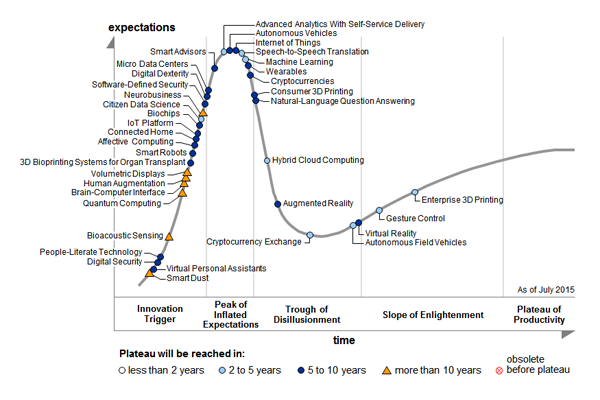
\includegraphics[width=0.9\textwidth]{imagens/gartner.png}
  \label{fig:gartner}
  
  Fonte: \cite{gartner}
\end{figure}

O conceito de casa inteligente � definido por \cite{jiang2004} como "uma resid�ncia incorporando uma rede de comunica��es que conecta servi�os e equipamentos el�tricos, permitindo que eles sejam controlados remotamente, monitorados ou acessados". Esta defini��o explicita o car�ter interativo e automatizado inerente ao conceito, abrindo uma margem muito grande de poss�veis aplica��es de utilidade social. Dentre tais aplica��es, inclui-se prover automa��o residencial e conectividade social \cite{harper2006}, al�m de fornecer um ambiente seguro e monitor�vel a idosos ou deficientes \cite{chan2008}.


\section{Solu��es existentes}\label{sec:solutions}
Acompanhando a populariza��o do conceito de \textit{smart houses}, diversas solu��es e plataformas foram desenvolvidas e lan�adas no mercado. Como exemplos, pode-se citar o Apple HomeKit \cite{homekit}, Wireless Sensor Tags \cite{wsensortags}, WigWag \cite{wigwag} e o Samsung SmartThings \cite{smartthings}.

Todas as solu��es citadas, � exce��o do Apple HomeKit, seguem uma arquitetura similar. Os sensores e atuadores distribu�dos pela resid�ncia s�o conectados a um controlador central , respons�vel por coletar leituras dos sensores e comandar a��es aos atuadores. Al�m disso, este controlador se conecta a um servidor em nuvem, que centraliza o armazenamento de dados e fornece uma interface aos usu�rios para monitorar e definir o estado da resid�ncia.

A solu��o desenvolvida pela Apple baseia-se na utiliza��o dos dispositivos m�veis da empresa para efetuar o monitoramento e controle mencionados. Assim, ela � fortemente dependente do ecossistema Apple para o funcionamento, especialmente pelo fato de o suporte ser dado somente pelo sistema operacional propriet�rio iOS. No entanto, a empresa permite o desenvolvimento de dispositivos de terceiros compat�veis com o HomeKit, atrav�s da disponibiliza��o de um \textit{framework} pr�prio. Os produtos desenvolvidos devem ser certificados pela Apple, processo este envolvendo a obten��o de licen�as e submiss�o a an�lises.

O Wireless Sensor Tags apresenta uma solu��o baseada em um controlador local (\textit{tag manager}) conectado � Internet, disponibilizando diversos sensores compat�veis com o controlador. Basicamente, ele permite a utiliza��o de um aplicativo para monitorar os sensores, definindo alertas de acordo com as leituras obtidas. N�o � mencionado suporte a atuadores, nem a possibilidade de desenvolver dispositivos de terceiros compat�veis com o sistema.

O WigWag tamb�m � uma solu��o baseada em um controlador local (aqui denominado \textit{relay}), podendo operar conectado � nuvem ou n�o. A interface dispon�vel possibilita a defini��o de regras de automa��o, controlando atuadores caso determinadas leituras de sensores forem verificadas. O aspecto mais interessante desta solu��o � a capacidade de integrar dispositivos de terceiros utilizando uma plataforma que se auto-denomina de c�digo  aberto, chamada deviceJS. No entanto, o acesso a esta plataforma se encontra fechado no momento de escrita deste relat�rio.

Por fim, de modo an�logo �s demais, a solu��o SmartThings baseia-se em um controlador local (\textit{hub}), que se conecta a servidores em nuvem pr�prios da Samsung. Esta solu��o destaca-se pelo foco dado � integra��o com dispositivos de terceiros, possuindo a documenta��o mais completa dentre os exemplos analisados. Tal integra��o baseia-se em dois componentes de software b�sicos: \textit{device handlers} e \textit{smart apps}. Os \textit{device handlers} funcionam como \textit{drivers}, sendo executados no controlador local. A fun��o deles � traduzir comandos de alto n�vel do controlador (e.g., ligar a luz) para sinais de controle espec�ficos do dispositivo. Os \textit{smart apps}, por sua vez, adicionam a parte de intelig�ncia do sistema, permitindo a cria��o de regras de automa��o de modo similar ao WigWag. A empresa disponibiliza aos desenvolvedores um ambiente de desenvolvimento completo para implementar os componentes citados.

\section{Motiva��o e Objetivos}\label{sec:goals}
Conforme mencionado, o conceito de \textit{smart houses} tem o potencial de trazer v�rios benef�cios aos usu�rios. Logo, � interessante incentivar o desenvolvimento de sistemas abertos, desvinculando-os de empresas e servi�os espec�ficos e tornando-os mais flex�veis para o usu�rio. Note que, das solu��es apresentadas, nenhuma � genuinamente aberta. As solu��es WigWag e Samsung SmartThings s�o as que mais se aproximam dessa ideologia ao disponibilizar plataformas em c�digo aberto para integrar dispositivos de terceiros, mas ainda possuem protocolos de comunica��o fechados (ao menos n�o documentados) e s�o dependentes de servidores em nuvem pr�prios.

Al�m disso, a intelig�ncia contida nas \textit{smart houses} � razoavelmente limitada nas solu��es existentes. Conforme apresentado anteriormente, toda a intelig�ncia � provida pelo usu�rio, que configura manualmente regras envolvendo sensores e atuadores. Ou seja, uma casa que se autoconfigurasse ou sugerisse regras ou a��es ao usu�rio teria destaque no mercado, eliminando ainda mais a interven��o do usu�rio e fornecendo ainda assim uma  experi�ncia altamente customizada.

Um �ltimo aspecto a se mencionar � o fato de nenhuma das solu��es estar dispon�vel no mercado brasileiro no momento de escrita deste relat�rio (in�cio de 2016). Os equipamentos do SmartThings, por exemplo, nem sequer s�o enviados ao Brasil, estando, pois, indispon�veis para importa��o. V�-se a necessidade, portanto, do desenvolvimento de uma solu��o nacional para o segmento das \textit{smart houses}.

Assim, pode-se dividir o objetivo do presente projeto nos seguintes itens:
\begin{enumerate}[\quad (i)]
	\item Projetar e implementar um \textbf{protocolo aberto de comunica��o em n�vel de aplica��o} para ser utilizada em uma rede de sensores sem fio voltada � automa��o residencial, e
	\item Projetar e implementar um \textbf{algoritmo de aprendizagem de m�quina ou minera��o de dados} de modo a prover automa��o residencial.
\end{enumerate}

%TODO Definir o escopo do projeto
\chapter{Especifica��o}

\section{Divis�o do Projeto}
O projeto pode ser dividido em dois sub-projetos, cada qual lidando com um objetivo listado na se��o anterior. O primeiro sub-projeto tem a finalidade de estruturar uma \textbf{rede de sensores} e atuadores utilizando um protocolo aberto, conforme descreve o objetivo i. O segundo sub-projeto busca desenvolver um \textbf{servi�o em nuvem} que agregue os dados coletados pela rede de sensores, efetuando, entre outras atividades, o processo de aprendizagem descrito no objetivo ii.

A especifica��o do projeto ser� feita por meio de requisitos funcionais e n�o-funcionais, que est�o listados em tr�s classes:
\begin{itemize}
	\item Requisitos de sistema, relativos � integra��o de ambos os sub-projetos;
	\item Requisitos da rede de sensores, referente ao sub-projeto dedicado a atingir o objetivo i; 
	\item Requisitos do servi�o em nuvem, referente ao sub-projeto dedicado a atingir o objetivo ii.
\end{itemize}

\section{Requisitos Funcionais} \label{sec:reqfunc}
\subsection{De sistema}
\begin{itemize}
	\item O sistema deve coletar dados do ambiente domiciliar e possibilitar a ativa��o de atuadores automaticamente ou por a��o humana;
	\item O sistema deve permitir que o usu�rio visualize o estado atual do sistema;
	\item O sistema deve se adaptar a altera��es de gostos e prefer�ncias do usu�rio.
\end{itemize}

\subsection{Da rede de sensores}
\begin{itemize}
	\item Toda a comunica��o deve ser realizada atrav�s de um protocolo �nico e formalizado;
	\item O protocolo de comunica��o deve permitir a identifica��o dos dispositivos da rede, bem como o envio de dados e de comandos de atua��o.
\end{itemize}

\subsection{Do servi�o em nuvem}
\begin{itemize}
	\item Permitir acesso remoto em qualquer localiza��o para que usu�rio controle seus dispositivos � dist�ncia;
	\item Aprender os h�bitos do usu�rio e configurar a rede de sensores automaticamente para realizar os seus gostos.

\end{itemize}

\section{Requisitos N�o-Funcionais} \label{sec:reqnfunc}
\subsection{De sistema}
\begin{itemize}
	\item F�cil instala��o de sensores e integra��o com a nuvem;
	\item Utilizar linguagens, ambientes e bibliotecas abertas.
\end{itemize}

\subsection{Da rede de sensores}
\begin{itemize}
	\item O protocolo de comunica��o desenvolvido deve ser aberto, de modo que qualquer fabricante possa criar um dispositivo que compat�vel com a rede;
	\item Deve possibilitar o uso de diversas tecnologias de comunica��o, tais como ZigBee, 802.15.4, e UDP;
	\item O protocolo deve gerar pacotes de tamanhos compat�veis com tecnologias de redes existentes para redes de sensores sem fio;
	\item A rede deve continuar operante mesmo sem acesso � nuvem.
\end{itemize}

\subsection{Do servi�o em nuvem}
\begin{itemize}
	\item Disponibilidade de 99\% do tempo; 
	\item API que possibilite o acesso atrav�s de aplica��es de terceiros/aplicativo/site.
\end{itemize}
\chapter{Projeto da Rede de Sensores}\label{chp:redesensores}
Este cap�tulo tem como fim elaborar o protocolo de comunica��o em n�vel de aplica��o, de modo a alcan�ar o objetivo (i) do trabalho. Este item objetiva especificar aspectos como o formato e conte�do das mensagens a serem transmitidas entre os dispositivos, provendo interoperabilidade entre os dispositivos aderentes � especifica��o.

A se��o \ref{sec:relwork} analisa protocolos existentes de aplica��o voltados a rede de sensores sem fio, bem como \textit{frameworks} existentes que utilizam tais tecnologias. Em seguida, discutem-se na se��o \ref{sec:commprot} protocolos de rede existentes que podem ser utilizados em conjunto com os protocolos de aplica��o para prover a comunica��o entre os dispositivos.

\section{Trabalhos relacionados}\label{sec:relwork}
Esta se��o tem como objetivo efetuar um estudo dos protocolos de aplica��o e \textit{frameworks} existentes para programa��o de redes de sensores. Os protocolos analisados a seguir permitem programar redes de sensores de prop�sito geral. O objetivo, ent�o, � analisar as caracter�sticas destes protocolos existentes para embasar o desenvolvimento de um protocolo espec�fico para redes de sensores voltados � automa��o residencial, que s�o alvos deste trabalho.

\subsection{Protocolos de Aplica��o existentes}
\paragraph*{CoAP.} O CoAP (Constrained Application Protocol) \cite{rfc7252} � um protocolo de aplica��o baseado no modelo REST que prov� transfer�ncia de dados entre n�s com recursos limitados. Suas mensagens seguem um formato similar ao HTTP, possuindo os tipos GET, POST, PUT e DELETE para efetuar opera��es sobre dados. Assim, por exemplo, um dado de um sensor pode ser obtido enviando a ele uma requisi��o GET do dado desejado. Uma caracter�stica importante do CoAP � o fato de ele ter sido projetado para funcionar sobre UDP, classificado como um protocolo de transporte n�o-confi�vel. Assim, o CoAP prov� recursos de confiabilidade, definindo mensagens confirm�veis que requerem a emiss�o pacotes do tipo ACK, confirmando a recep��o de tais mensagens.

\paragraph*{MQTT.} O MQTT (Message Queue Telemetry Transport) \cite{mqtt} � um protocolo de aplica��o aplicando o modelo publicador/observador (\textit{publisher/subscriber}) para transfer�ncia de dados. Nesse sistema, existem tr�s tipos de elementos: publicadores, observadores e um elemento intermedi�rio (\textit{broker}) de coordena��o, como pode ser visto na Figura \ref{fig:mqtt}. Os dispositivos publicadores registram os dados gerados no coordenador, e os observadores registram interesse em receber dados de determinados publicadores. O coordenador, ent�o, encaminha os dados dos publicadores para os observadores interessados. 

\begin{figure}[h]
	\centering
	\caption{Arquitetura do protocolo MQTT}
  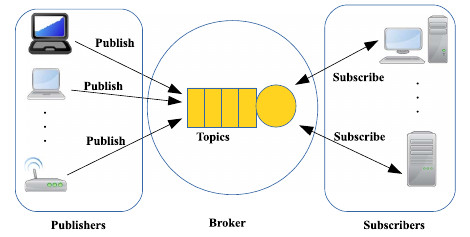
\includegraphics[width=0.8\textwidth]{imagens/mqtt.png}
  \label{fig:mqtt}  
  
  Fonte: \cite{Fuqaha2015}
\end{figure}

\paragraph*{DDS.} O DDS (Data Distribution Service) \cite{dds} � um protocolo de aplica��o que tamb�m aplicao modelo publicador/observador, mas, ao contr�rio do MQTT, n�o envolve um elemento coordenador. Este protocolo prev� o envio de mensagens por multicast, sendo adequado a redes com requisitos de tempo real no contexto de IoT, al�m de prover diversos par�metros de qualidade de servi�o.

A Tabela \ref{tab:comp_prot_aplic} resume as caracter�sticas principais dos protocolos de aplica��o analisados. Observe que os protocolos apresentados se baseiam sobre TCP ou UDP, implicando em restri��es quanto � sua utiliza��o com protocolos de comunica��o que n�o s�o baseados neles. 

\begin{table}[h]
	\centering
	\caption{Compara��o dos Protocolos de Aplica��o analisados}\smallskip
	\label{tab:comp_prot_aplic}
	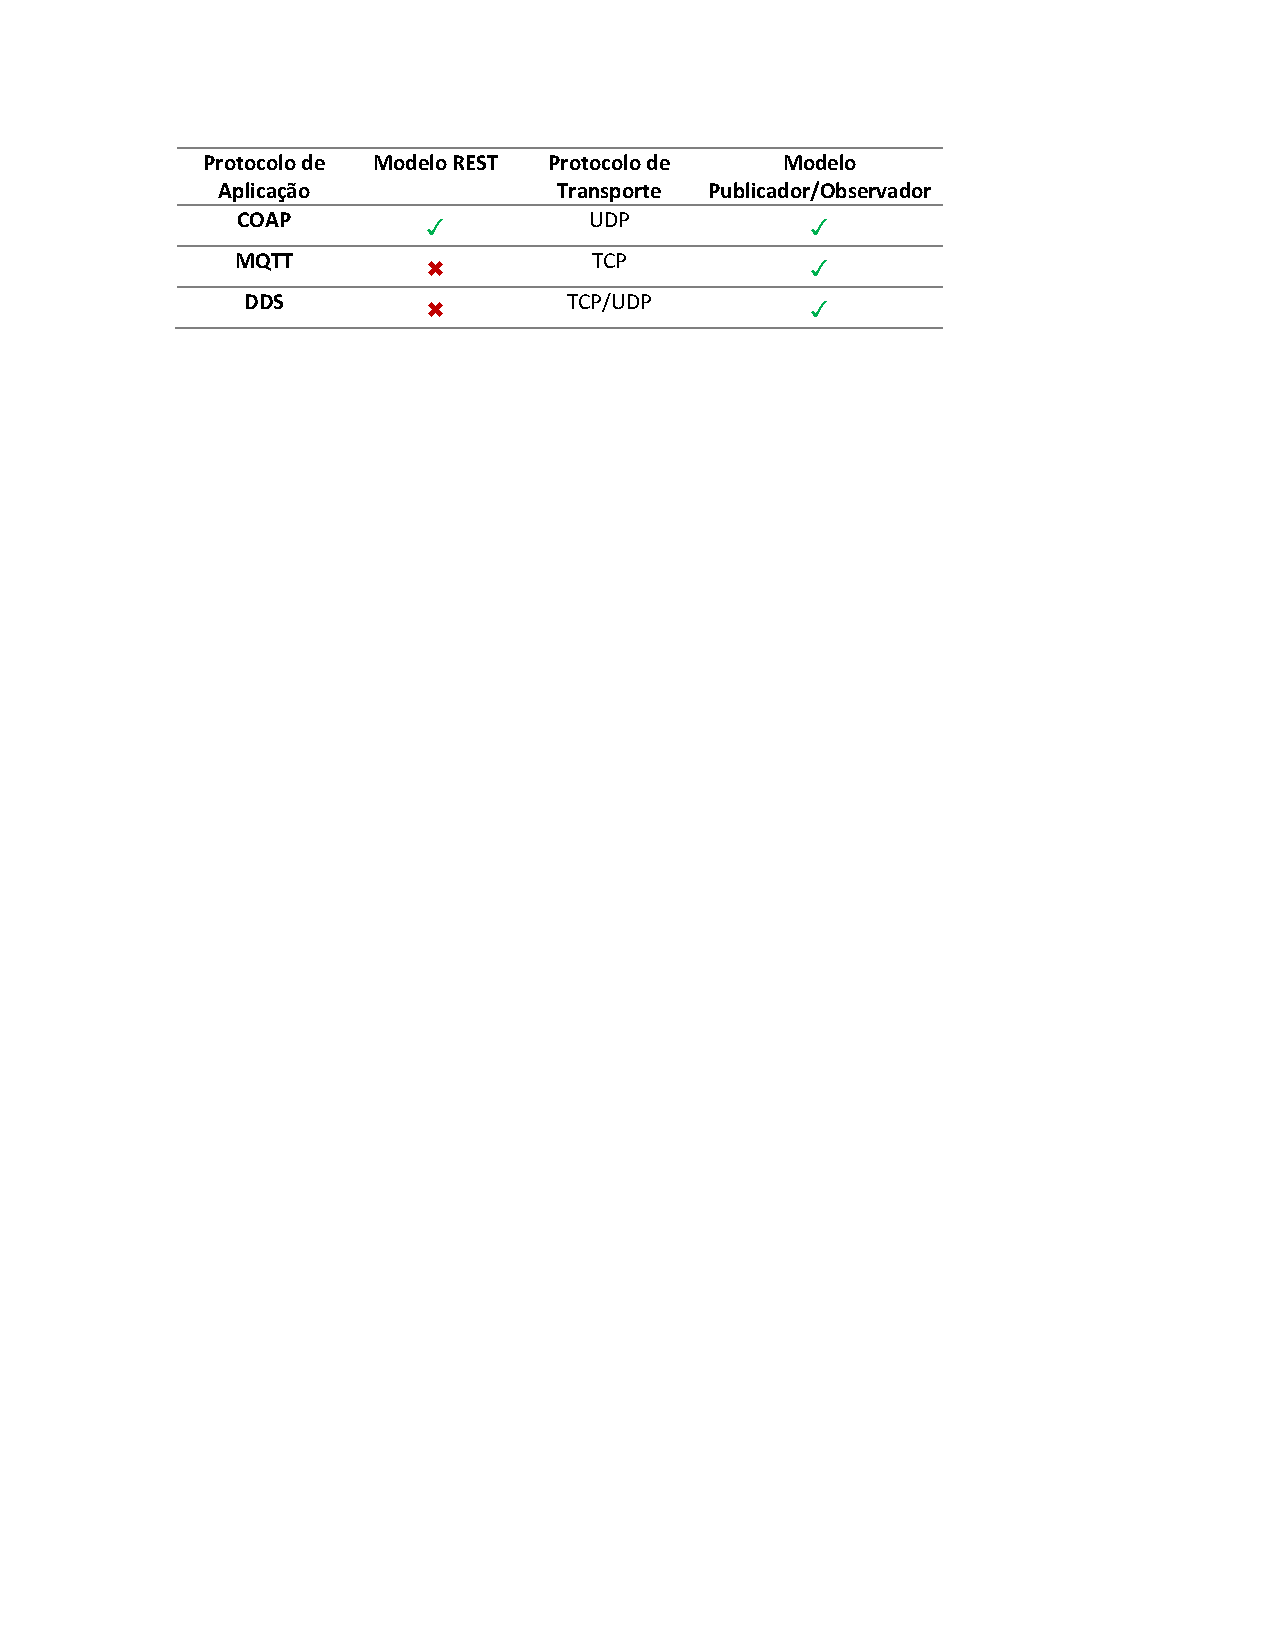
\includegraphics[width=\textwidth]{tabelas/comp_prot_aplic.pdf}
	
	Fonte: \cite{Fuqaha2015}
\end{table}

\subsection{\textit{Frameworks} existentes}
\paragraph*{IoTivity.} O IoTivity \cite{iotivity} � um projeto colaborativo da funda��o Linux que tem por objetivo prover um padr�o para prover conectividade entre dispositivos no contexto de internet das coisas. Suas funcionalidades incluem prover descoberta de dispositivos, transmiss�o de dados, gerenciamento de dispositivos e gerenciamento de dados, como ilustra a \ref{fig:iotivity}. Seu funcionamento se baseia em uma arquitetura REST (baseado no CoAP), por meio da qual dados e mensagens de controle s�o trafegadas. 

\begin{figure}[h]
	\centering
	\caption{Arquitetura do projeto IoTivity}
  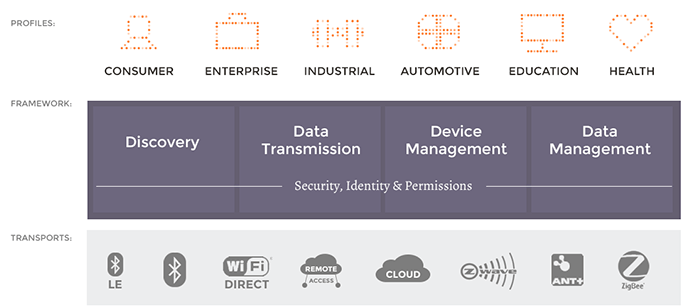
\includegraphics[width=0.8\textwidth]{imagens/iotivity.png}
  \label{fig:iotivity}  
  
  Fonte: \cite{iotivity}
\end{figure}

Uma caracter�stica proposta na arquitetura do IoTivity a ser adotada neste projeto � a cria��o de uma interface comum a v�rios protocolos de rede subjacentes, visto que prov� flexibilidade � tecnologia de comunica��o adotada pelos dispositivos. Entretanto, n�o se deseja adotar a abordagem REST utilizada no IoTivity, pois isso implica que todos os dispositivos necessitam escutar requisi��es continuamente. 

\paragraph*{ARM mbed.} O mbed \cite{mbed} � uma plataforma de desenvolvimento da ARM, que prov� um ecossistema para desenvolvimento de aplica��es em IoT. Um de seus produtos principais � o sistema operacional mbed OS, compat�vel somente com dispositivos baseados no microprocessador ARM Cortex-M. Este sistema prov� um ambiente de execu��o baseado em eventos e suporta diversos protocolos de rede (Ethernet, Wi-Fi, 6loWPAN, Thread e Bluetooh LE), seguran�a e gerenciamento de dispositivos baseados em REST.

A plataforma mbed � relativamente complexa, provendo, al�m do sistema operacional citado, ferramentas de empacotamento de aplica��es, de testes automatizados e de integra��o com servi�os  em nuvem. Sua principal desvantagem � a restri��o de processadores suportados, que apesar de ampla, restringe significativamente a flexibilidade dos dispositivos utilizados em uma rede. 

\paragraph*{RIOT.} O RIOT \cite{baccelli2013} � um sistema operacional que permite programar dispositivos utilizando  C ou C++, possibilitando utilizar ferramentas populares entre programadores como o compilador gcc e o depurador gdb. Ele prov� suporte a diversas plataformas, al�m de prover implementa��es de diversas pilhas de rede (6LoWPAN, IPv6, UDP) e protocolos de aplica��o tais como CoAP que podem ser inclu�dos nos programas caso necess�rios.

Uma desvantagem do RIOT � o fato de o seu uso estar restrito �s plataformas suportadas, que apesar de estarem em expans�o, n�o incluem, at� o momento de escrita deste relat�rio, dispositivos de prototipa��o populares tais como o Arduino Uno e Raspberry Pi. Al�m disso, seu uso est� restrito a processadores com um �nico n�cleo, inviabilizando a utiliza��o de dispositivos mais recentes. 
 
\section{Protocolos de rede existentes}\label{sec:commprot}
O projeto de uma rede de sensores e atuadores sem fio deve levar em conta diversas restri��es dos dispositivos que a comp�em, tais como o acesso limitado a uma fonte de energia, capacidade reduzida de processamento e meio de comunica��o com interfer�ncias. Com estas restri��es em mente, diversos protocolos de comunica��o foram propostos para viabilizar a implementa��o de redes de sensores sem fio, descritos a seguir.

\subsection{ZigBee}
O ZigBee � um protocolo de comunica��o proposto e padronizado pela \textit{ZigBee Alliance} em 2003, visando aplica��o em redes de sensores sem fio \cite{zigbeealliance}. A especifica��o do protocolo abrange diversos aspectos, desde os de natureza f�sica (e.g., estrat�gias de redu��o de interefer�ncia) �s de natureza de aplica��o (e.g., aplica��o de criptografia sobre os dados transmitidos) \cite{stevanovic2007}. A Figura \ref{fig:zigbee} ilustra a abrang�ncia do protocolo ZigBee, tendo como base um modelo em camadas de rede similar ao OSI.

\begin{figure}[h]
	\centering
	\caption{Abrang�ncia da especifica��o do protocolo ZigBee, baseado em um modelo de camadas.}
  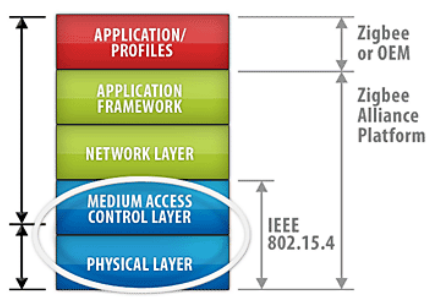
\includegraphics[width=0.8\textwidth]{imagens/zigbee.png}
  \label{fig:zigbee}
  
  Fonte: \cite{stevanovic2007}
\end{figure}

Como pode ser verificado no esquema, o ZigBee baseia-se na especifica��o IEEE 802.15.4 no que tange �s camadas f�sica e de controle de acesso ao meio (equivalente �s camadas 1 e 2 do modelo OSI). O ZigBee define somente aspectos de alto n�vel que comp�em as camadas de rede (camada 3) e de aplica��o. Nos pr�ximos par�grafos, ser� feita uma descri��o do 802.15.4.

O protocolo IEEE 802.15.4 � um protocolo de camadas f�sica e de enlace que busca prover comunica��o com baixa complexidade para dispositivos com capacidades limitadas de transmiss�o de dados e de processamento \cite{ieee802_15}. A Tabela \ref{tab:802} resume as caracter�sticas deste protocolo.

\begin{table}[h]
	\centering
	\caption{Caracter�sticas do protocolo IEEE 802.15.4}\smallskip
	\label{tab:802}
	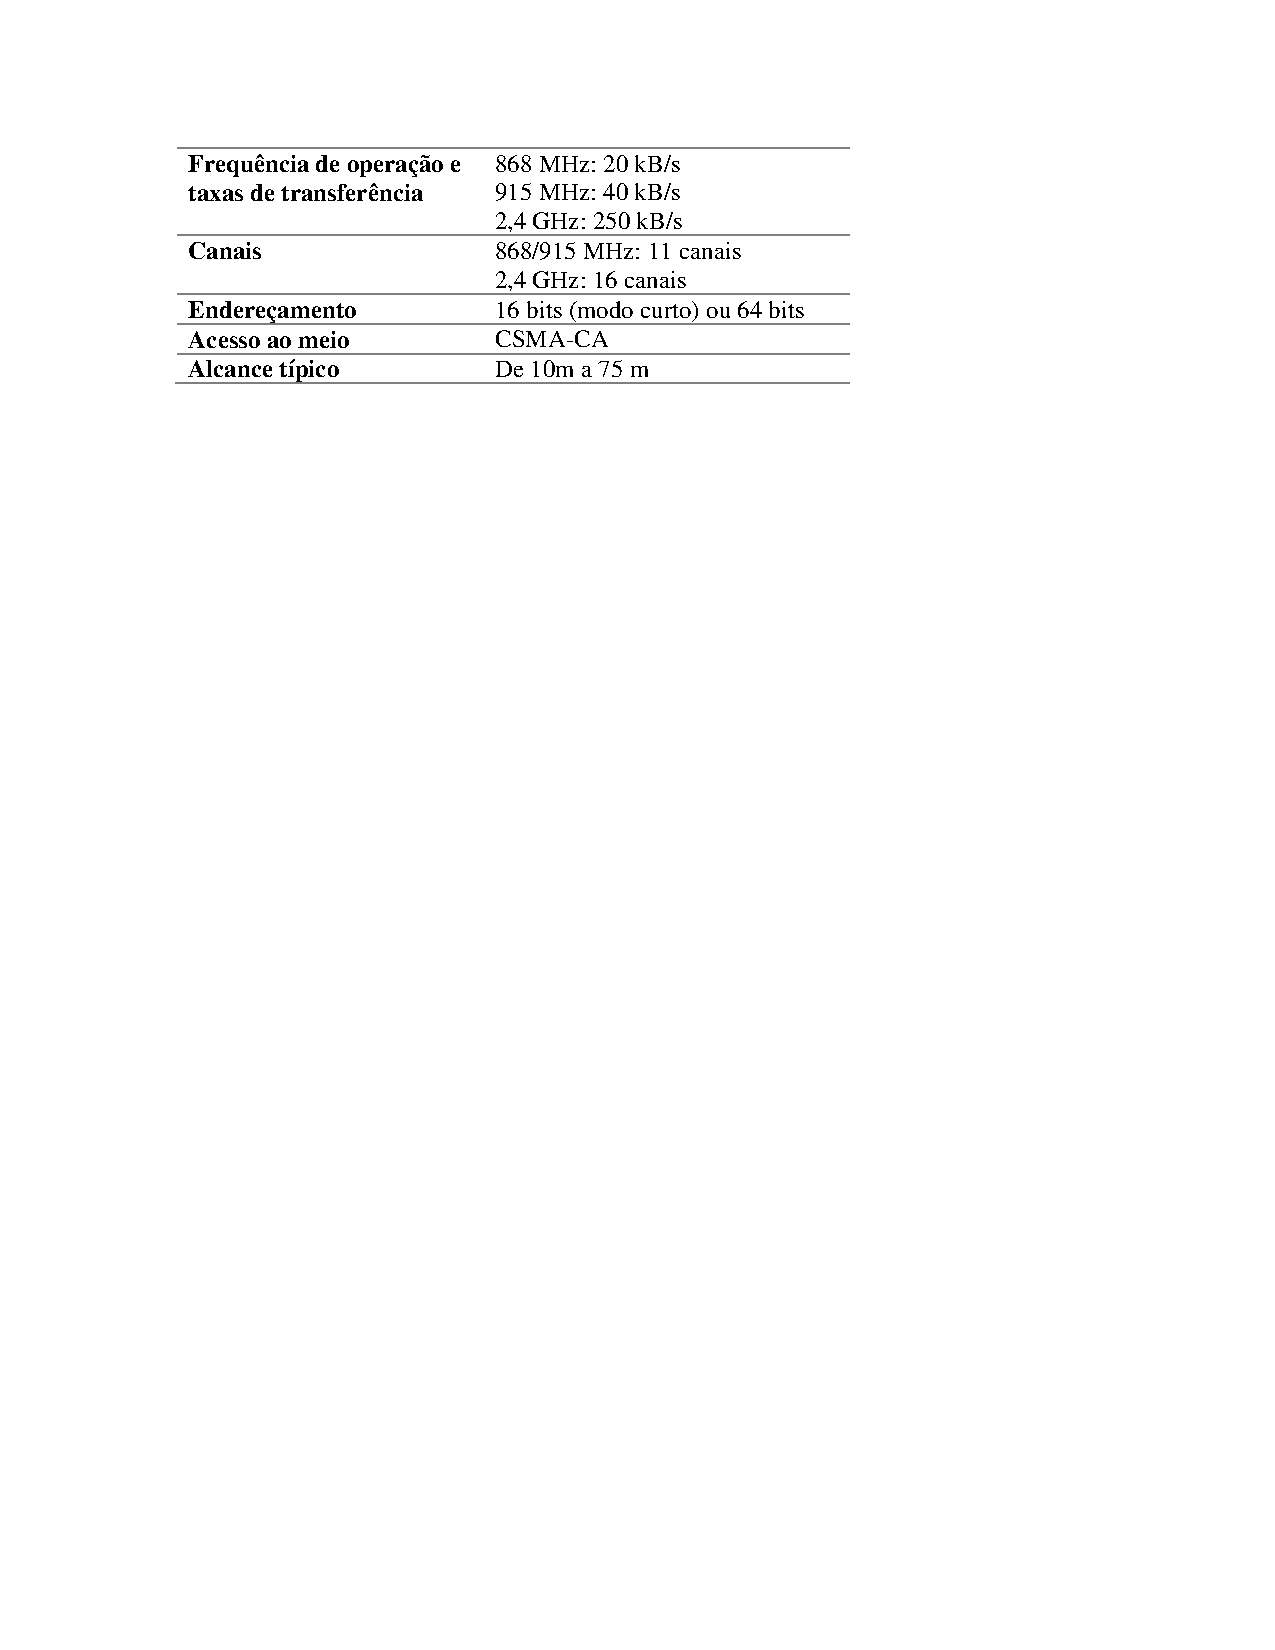
\includegraphics[width=0.8\textwidth]{tabelas/802_15_4.pdf}
	
	%\bigskip
	Fonte: \cite{stevanovic2007, schonwalder2010}
\end{table}
Como se pode notar, o protocolo opera em tr�s faixas de frequ�ncia, sendo que a de 2,4 GHz prov� maior n�mero de canais e maior vaz�o de dados, al�m de estar licenciado para uso global, ao contr�rio das demais \cite{schonwalder2010}. Dentre as fun��es desempenhadas pelo 802.15.4, destacam-se o controle de acesso ao canal (baseado no CSMA-CA), a confirma��o de entrega e checagem de erro em \textit{frames}.

O protocolo IEEE 802.15.4 ainda define dois tipos de dispositivos. Um dispositivo com funcionalidade completa (\textit{Full Function Device - FFD}) n�o possui restri��es acentuadas de recursos, podendo se tornar um n� coordenador da rede de sensores. Ele pode efetuar diversas tarefas dentro da rede, tal como aceitar conex�es e encaminhar pacotes. 

Um dispositivo com funcionalidade reduzida (\textit{Reduced Function Device - RFD}), por sua vez, consiste em um dispositivo perif�rico, tal como um sensor, possuindo restri��es significativas de recursos. Estes dispositivos em geral atuam como "folhas" na topologia de rede, comunicando-se com um n� concentrador (um FFD) quando necess�rio.

Conforme mencionado, o ZigBee define recursos das camadas de rede e aplica��o, como uma extens�o ao protocolo 802.15.4 (ver Figura \ref{fig:zigbee}). Para tanto, s�o definidos tr�s tipos de equipamentos dentro de uma rede ZigBee. Um dispositivo final consiste em um FFD ou RFD simples, que se comunica com um �nico n�. Um dispositivo roteador � um FFD capaz de reencaminhar mensagens  ao destinat�rio, caso necess�rio. Por fim, um dispositivo coordenador atua como coordenador da rede, possuindo tamb�m as funcionalidades de um roteador.

Pode-se derivar um recurso importante introduzido pela especifica��o do ZigBee: o roteamento \textit{multihop}, atuando como camada de rede. Isso significa que caso um dispositivo envie um pacote para outro esteja fora do seu alcance, basta que haja roteadores conectando-os. Al�m disso, o ZigBee permite a forma��o de redes em malha (\textit{mesh}), provendo confiabilidade e toler�ncia a falhas.

Por fim, o ZigBee introduz recursos importantes em n�vel de aplica��o. Exemplos incluem a possibilidade de fragmenta��o e remontagem de pacotes, manuten��o de um registro de dispositivos pareados e funcionalidades relacionadas � seguran�a, como criptografia.

\subsection{6LoWPAN}
O 6LoWPAN � um protocolo definido pelo IETF que define a utiliza��o de IPv6 sobre redes sem fio de baixo consumo, de alcance pessoal (acr�nimo do ingl�s \textit{IPv6 over Low-power Wireless Personal Area Network}) \cite{rfc4944}. O objetivo principal deste protocolo � integrar o protocolo IP em redes de baixo consumo, trazendo diversos benef�cios, tais como \cite{rfc4919, schonwalder2010}
\begin{itemize}
	\item A possibilidade de se reutilizar a infraestrutura IP existente;
	\item A possibilidade de adotar tecnologias que trabalham sobre o protocolo IP, em geral amplamente conhecidos e aceitos por profissionais;
	\item A facilidade de interoperabilidade com redes IP existentes, e
	\item A adequa��o do esquema de endere�amento do IPv6, suprindo a necessidade de um grande n�mero de endere�os exigido em uma aplica��o de IoT.
\end{itemize}

De modo semelhante ao ZigBee, o 6LoWPAN baseia-se no protocolo IEEE 802.15.4 no que tange �s camadas f�sica e de enlace, de modo a se adequar a redes de baixo consumo. No entanto,o 6LoWPAN define uma camada de interface entre as camadas do 802.15.4 e IP, como pode ser visto na Figura \ref{fig:6lowpan}.

\begin{figure}[h]
	\centering
	\caption{A especifica��o do protocolo 6LoWPAN e sua rela��o com os protocolos 802.15.4 e IP. O modelo OSI � mostrado ao lado como refer�ncia.}
  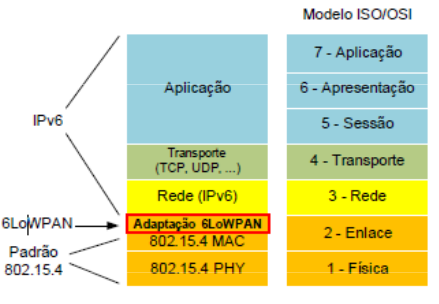
\includegraphics[width=0.8\textwidth]{imagens/6lowpan.png}
  \label{fig:6lowpan}
  
  Fonte: \cite{moreiras2009}
\end{figure}

A necessidade de uma camada de interface entre o IPv6 e as camadas inferiores padronizadas pelo 802.15.4 se d� por incompatibilidades existentes entre tais protocolos \cite{rfc4919}. Um exemplo diz respeito ao tamanho dos pacotes previstos por cada protocolo: o 802.15.4 prev� pacotes pequenos, com tamanhos de no m�ximo 81 bytes, ao passo que o IPv6 exige suporte a um MTU m�nimo de 1280 bytes. Logo, um papel da interface definida pelo 6LoWPAN � o de efetuar fragmenta��o e montagem dos pacotes, a fim de compatibilizar os protocolos.
Outras fun��es do protocolo incluem:
\begin{itemize}
	\item Compress�o de cabe�alho: como mencionado, o 802.15.11 suporta cabe�alhos de no m�ximo 81 bytes. Sendo que um cabe�alho IPv6 ocupa no m�nimo 40 bytes (sem os cabe�alhos opcionais), restam somente 41 bytes para serem usados pelos protocolos de camadas superiores. Fica evidente, ent�o, a necessidade de se aplicar t�cnicas de compress�o de cabe�alho, fun��o esta desempenhada pelo 6LoWPAN;
	\item Roteamento \textit{multi-hop} em redes \textit{mesh}: de modo semelhante ao ZigBee, o 6LoWPAN permite a configura��o de redes \textit{mesh} com capacidade de  autorrepara��o, provendo robustez.
\end{itemize}

\subsection{Bluetooth}
Bluetooth � uma tecnologia de comunica��o sem fio a curta dist�ncia. Opera em banda n�o licenciada ISM (Industrial, Cient�fica e M�dica, na sigla em ingl�s) entre 2,4Ghz e 2,485GHz.
Por n�o utilizar banda licenciada, o Bluetooth utiliza saltos adaptativos em frequ�ncia (\textit{Adaptative Frequency Hoping} - AFH) para diminuir a interfer�ncia com outros dispositivos operantes na mesma faixa de 2,4GHz. O aparelho toma conhecimento de demais dispositivos na mesma frequ�ncia e as evita, saltando entre 79 frequ�ncias a intervalos de 1MHz \cite{redesbluetooth}. 

A opera��o Bluetooth ocorre em redes Ad-Hoc de curto alcance conhecidas como Piconet. Tais redes podem ser constitu�das por 1 membro mestre, 7 escravos ativos e 248 escravos estacionados (endere�amento de 8 bits). Cada dispositivo pode pertencer a v�rias Piconets. 
Seu raio de opera��o depende do dispositivo utilizado, que pode ser classificado em tr�s categorias:
\begin{itemize}
        \item Classe 3: alcance de 1 metro e pot�ncia m�xima de 1mW.
        \item Classe 2: alcance de 10 metros e pot�ncia m�xima de 2,5mW.
        \item Classe 1: alcance de 100 metros, pot�ncia m�xima de 100mW.
\end{itemize}

A camada mais baixa da arquitetura Bluetooth � a camada F�sica, na qual s�o definidas as especifica��es do dispositivo para operar. Dois dispositivos compartilham o mesmo meio f�sico e para se comunicarem devem estar sintonizados na mesma frequ�ncia (processo de parear). Para identificar os membros da Piconet, um c�digo de acesso � sempre enviado no cabe�alho de cada pacote, aumentando a carga e inviabilizando para dispositivos de menor capacidade, como no caso deste projeto. 

Uma mesma unidade pode participar como escrava em v�rias Piconets mas atuar como mestre em apenas uma. Para participar de mais de uma Piconet o dispositivo atua com multiplexa��o no tempo (\textit{Time Division Multiplex} - TDM). O conjunto de v�rias Piconets independentes e n�o sincronizadas � chamado de Scatternet, conforme esquematizado na \ref{fig:redesbluetooth}.

\begin{figure}[h]
	\centering
	\caption{Diagrama para rede Piconet e conjunto gerando Scatternet.}
  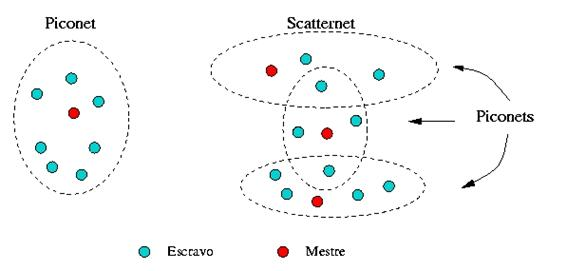
\includegraphics[width=0.8\textwidth]{imagens/redesbluetooth.jpg}
  \label{fig:redesbluetooth}
  
  Fonte: \cite{redesbluetooth}
\end{figure}

No acesso ao meio f�sico utiliza-se o m�todo CDMA (\textit{Code Division Multiple Access}). Para o projeto da casa conectada, utilizaria-se o padr�o de Enlace ACL (\textit{Asynchronous Conection-Less}), do tipo ponto-multiponto (um mestre e v�rios escravos). Este padr�o � adequado para transmiss�o de dados, de modo que pacotes perdidos ou com erros s�o retransmitidos. 

Em qualquer rede sem fio, a vulnerabilidade das informa��es � evidente. Como o meio que propaga o sinal � o pr�prio ar, um dispositivo pode captar um sinal sendo enviado se este n�o for devidamente protegido. No caso da tecnologia Bluetooth, onde as conex�es s�o feitas de forma autom�tica, � especialmente importante definir formas de proteger os usu�rios para que n�o recebam dados de dispositivos que n�o desejam.

Para garantir a integridade das informa��es, aplicam-se modos de criptografia e autentica��o. Isto � especialmente importante no projeto da casa conectada, no qual usu�rios externos e diferentes do dono do sistema n�o podem ter acesso aos dados trafegados. 

Para iniciar uma conex�o, um pedido de permiss�o deve ser enviado. Os dispositivos Bluetooth usam uma chave de acesso chamada n�mero de identifica��o pessoal (PIN) para autentica��o. Se a chave de acesso digitada pelo usu�rio que deseja conectar corresponder � chave de acesso ao dispositivo detectado, a autentica��o � realizada com �xito. Caso contr�rio ela falhar�. 

\subsection{Z-Wave}
Z-Wave � um protocolo de comunica��o sem fio que tem como foco baixo consumo, baixa taxa de dados e confiabilidade. Foi criado pela empresa dinamarquesa Zen-Sys, que foi adquirida pela Sigma Designs e desde sua concep��o � voltada para automa��o residencial \cite{wikizwave,zwavelayers}.

As duas camadas mais baixas (F�sica e Enlace) da pilha de protocolos s�o definidas pelo ITU-T G.9959, ou seja, trata-se de um padr�o formalmente definido por um �rg�o internacional de padr�es. Por�m, sua camada de rede � definida pela Sigma Designs e as camadas acima s�o definidas pelo desenvolvedor da aplica��o, como pode ser observado na Figura \ref{fig:zwavelayers}.


\begin{figure}[h]
	\centering
	\caption{Pilha de protocolos do Z-Wave}
  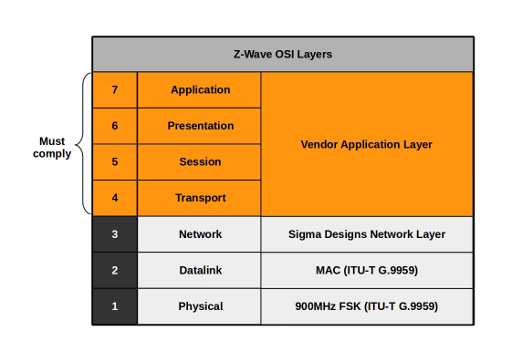
\includegraphics[width=0.8\textwidth]{imagens/zwavelayers.jpg}
  \label{fig:zwavelayers}
  
    Fonte: \cite{zwavelayers}
\end{figure}

O Z-Wave trabalha em frequ�ncias abaixo de 1GHz, por volta de 900MHz, fazendo com que ela n�o interfira com Wi-Fi, Bluetooth e diversas outras tecnologias que trabalham na j� bastante utilizada frequ�ncia de 2,4GHz. Al�m disso, suas taxas de transmiss�o s�o de 9600 bit/s, 40 kbit/s ou 100 kbit/s e seu alcance � de 100m em �reas abertas.

Uma rede Z-Wave define dois tipos de dispositivos: controladores e escravos. Os controladores iniciam comandos de controle para os escravos e os enviam. J� os n�s escravos apenas respondem a comandos e os executam. Por�m, estes n�s tamb�m podem funcionar como repetidores, aumentando o alcance de sua rede Z-Wave.

Cada rede Z-Wave pode conter at� 232 dispositivos e � identificada por um ID da rede (Network ID ou Home ID), que possui 32 bits. N�s conectados em redes distintas n�o podem se comunicar diretamente entre si, e em uma rede cada n� tem um ID �nico (Node ID) de 8 bits.

As redes Z-Wave utilizam uma topologia de malha (\textit{mesh}) e � necess�rio existir um controlador prim�rio e opcionalmente controladores secund�rios. Os n�s s�o adicionados atrav�s do pareamento em que o controlador mede a for�a do sinal entre os equipamentos e assume que esta ir� se manter constante, fazendo com que os escravos n�o possam se mover espacialmente sem terem que realizar o pareamento novamente.

\section{An�lise dos protocolos de comunica��o}
Uma vez descritos os protocolos de comunica��o, � poss�vel analisar as vantagens e desvantagens de cada um deles, tendo em vista o escopo do presente trabalho. A Tabela \ref{tab:analiseprotcom} lista de forma sucinta as caracter�sticas levantadas de cada protocolo.

\begin{table}[h]
	\centering
	\caption{An�lise dos protocolos de comunica��o}\smallskip
	\label{tab:analiseprotcom}
	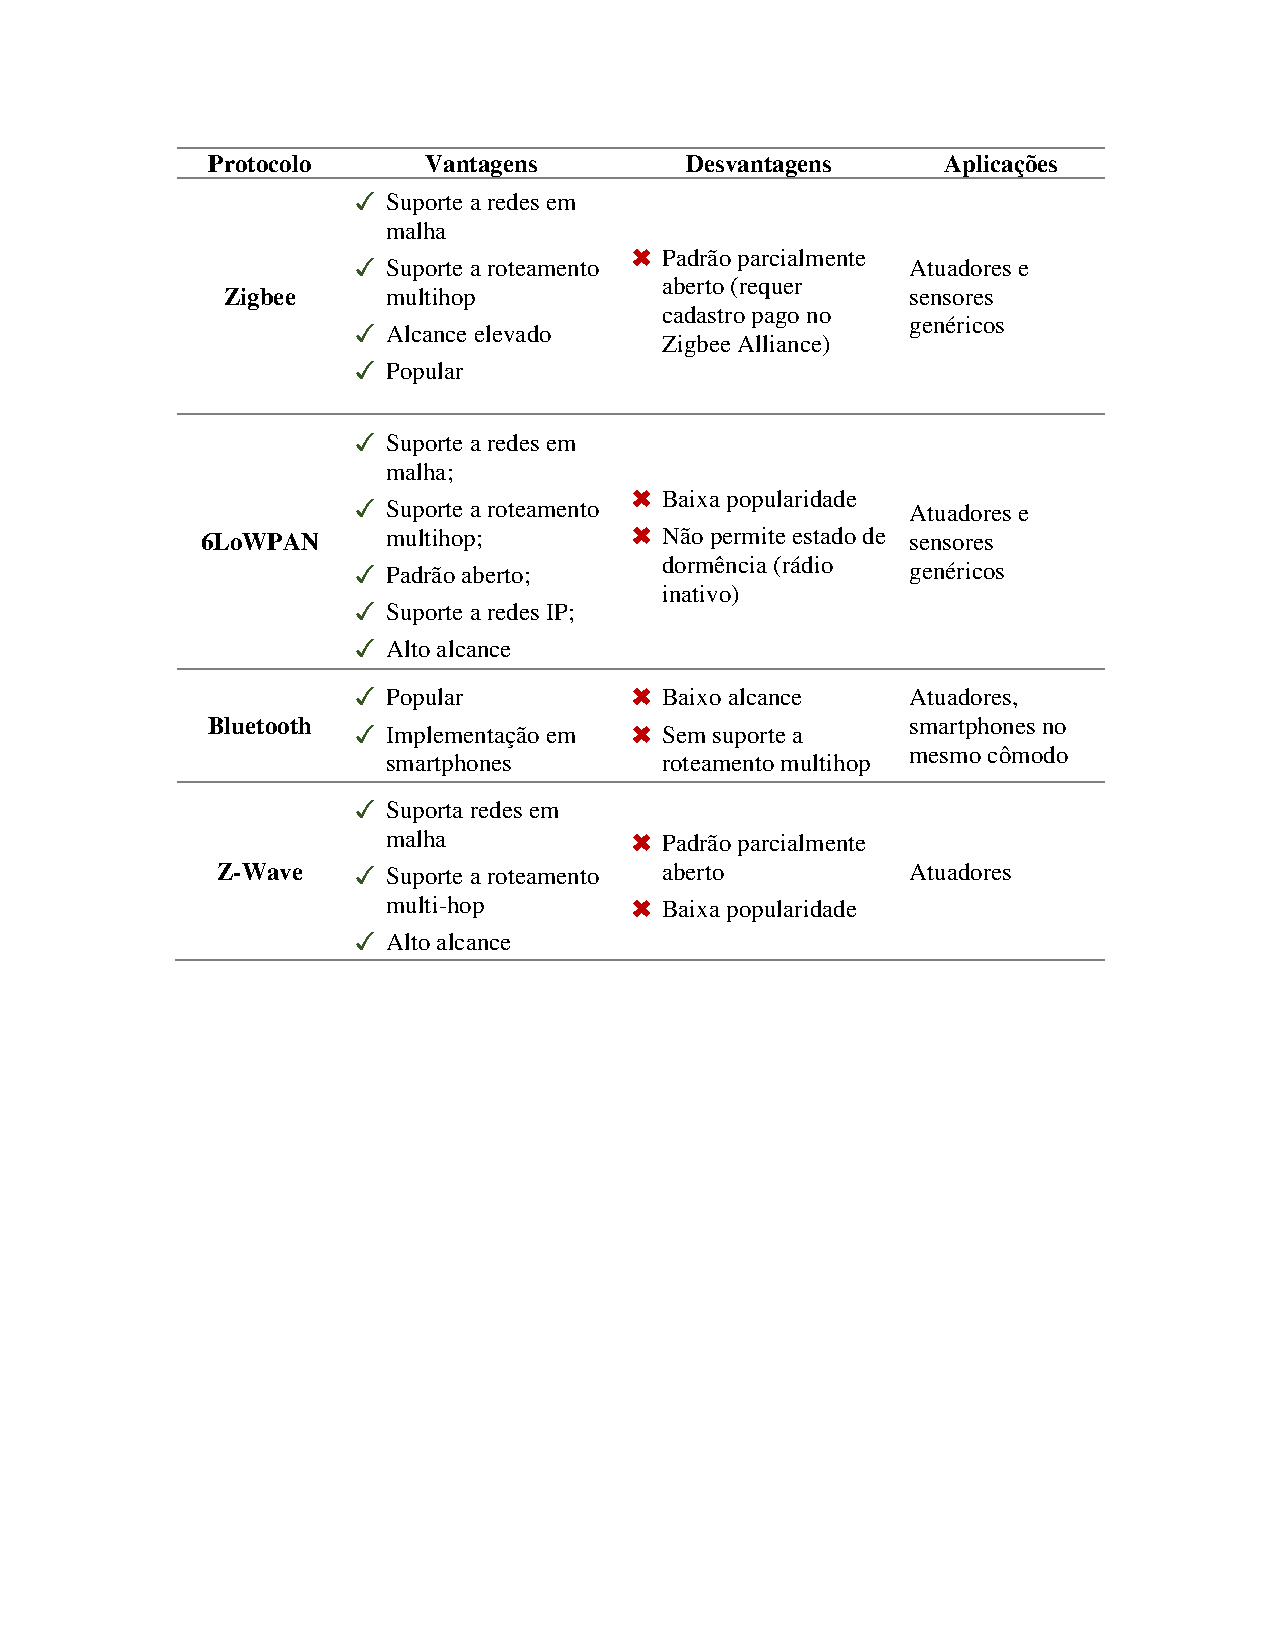
\includegraphics[width=\textwidth]{tabelas/comp_prot_rede.pdf}
\end{table}

Conforme mencionado, os protocolos ZigBee e 6LoWPAN s�o baseados no padr�o IEEE 802.15.4, apresentando, pois, caracter�sticas f�sicas e de acesso ao meio similares, tais como frequ�ncia de opera��o e alcance. Ambos ainda preveem suporte a redes em malha com roteamento \textit{multihop}, permitindo aplica��es em ambientes em que a localiza��o dos dispositivos seja esparsa, sendo necess�rio roteadores intermedi�rios para comunica��o.

No entanto, tais protocolos diferem entre si em alguns aspectos. Em primeiro lugar, o ZigBee foi padronizado em 2003, visto como o protocolo mais popular utilizado em redes de sensores sem fio \cite{toscano2012}. O 6LoWPAN, por sua vez, � um padr�o mais novo, tendo sido proposto pelo IETF em 2007. Al�m disso, a especifica��o do 6LoWPAN � totalmente aberta, al�m de adotar camadas de n�vel superior (rede e transporte) conhecidas e amplamente adotadas em redes existentes (IP e TCP/UDP), ao passo que o ZigBee define camadas de rede e aplica��o pr�prias, em uma especifica��o de acesso restrito. Por fim, o Zigbee prev� a possibilidade de os n�s entrarem em um estado de dorm�ncia (r�dio inativo), ao passo que o 6LoWPAN n�o permite este modo. Isto se deve ao fato de ele estar baseado no protocolo IP, que prev� que os n�s sempre estejam ativos \cite{toscano2012}.

Em rela��o ao Bluetooth, pode-se consider�-lo um protocolo amplamente difundido, sendo integrado inclusive em maior parte dos dispositivos m�veis atuais. No entanto, ele possui a desvantagem de possuir alcance limitado e de n�o suportar redes complexas, limitando a abrang�ncia da rede. Soma-se a isso o fato de n�o ser poss�vel iniciar a comunica��o de um dispositivo escravo a um mestre (coordenador), tornando inconveniente a utiliza��o de sensores como escravos, haja vista a necessidade de mant�-los ativos � espera de uma mensagem do dispositivo mestre para envio das leituras.

Por fim, nota-se que o Z-Wave possui vantagens em comum �s do ZigBee e do 6LoWPAN. Em contrapartida, sua especifica��o � parcialmente aberta, al�m de possuir baixa ado��o. De modo similar ao Bluetooth, este dispositivos atuando como escravos n�o podem iniciar uma comunica��o, devendo somente responder �s mensagens de um mestre.

%Ponderando as caracter�sticas expostas, o grupo optou por adotar o protocolo ZigBee para implementar um prot�tipo de rede a ser utilizado como base para projetar o protocolo de n�vel de aplica��o. Cabe ressaltar que o protocolo de aplica��o deve ser gen�rico a ponto de funcionar corretamente independente da escolha dos protocolos de comunica��o subjacentes.

\section{Defini��o do Protocolo de Aplica��o \textit{Rainfall}}
\subsection{Requisitos} \label{subsec:requisitos}
Uma vez analisados os protocolos de aplica��o e frameworks existentes (se��o \ref{sec:relwork}), bem como os protocolos de rede (se��o \ref{sec:commprot}), e tendo em vista os requisitos levantados para a rede de sensores (se��es \ref{sec:reqfunc} e \ref{sec:reqnfunc}), pode-se passar para a especifica��o do protocolo de aplica��o proposto, batizado de \textit{Rainfall}. Os requisitos relativos ao protocolo est�o reescritos abaixo, por fins de claridade.

\begin{enumerate}[\quad R1.]
	\item O protocolo a ser desenvolvido deve funcionar com diversos protocolos de rede. Conforme a an�lise realizada, existem diversos protocolos de redes voltados a redes de sensores sem fio existentes, e conv�m que o protocolo de aplica��o desenvolvido n�o seja restrito a nenhum deles de forma espec�fica. Uma abordagem similar � do IoTivity pode ser interessante, criando-se uma interface comum a v�rios protocolos de rede subjacentes;
	\item Os dispositivos devem poder declarar sua funcionalidade, incluindo informa��es sobre sua classifica��o como sensor ou atuador, e sua categoria (tipo de sensor ou atuador);
	\item Os dispositivos devem poder enviar dados de leitura (no caso de sensores) e receber comandos de atua��o (no caso de atuadores);
	\item O protocolo deve enviar mensagens de forma concisa, levando em considera��o as limita��es dos dispositivos envolvidos.
\end{enumerate}

\subsection{Sintaxe e Sem�ntica} \label{subsec:sintaxe}
Levando-se em conta a natureza das mensagens a serem transmitidas, conv�m adotar uma estrutura de dados no formato chave-valor. Neste relat�rio, a representa��o dos dados seguindo este formato ser� feito de forma similar ao formato JSON:
\begin{center}
	\texttt{\{chave\_1:valor\_1, ..., chave\_n:valor\_n\}}
\end{center}
onde \texttt{chave\_1}, \texttt{chave\_n} s�o as chaves e \texttt{valor\_1}, \texttt{valor\_n} s�o os valores associados.

Os requisitos definidos na se��o \ref{subsec:requisitos} permitem definir as chaves e valores associados a serem utilizados no protocolo, conforme mostra a Tabela \ref{tab:chavevalorprot}.

\begin{table}[h]
	\centering
	\caption{Chaves e valores associados utilizados no protocolo de aplica��o.}\smallskip
	\label{tab:chavevalorprot}
	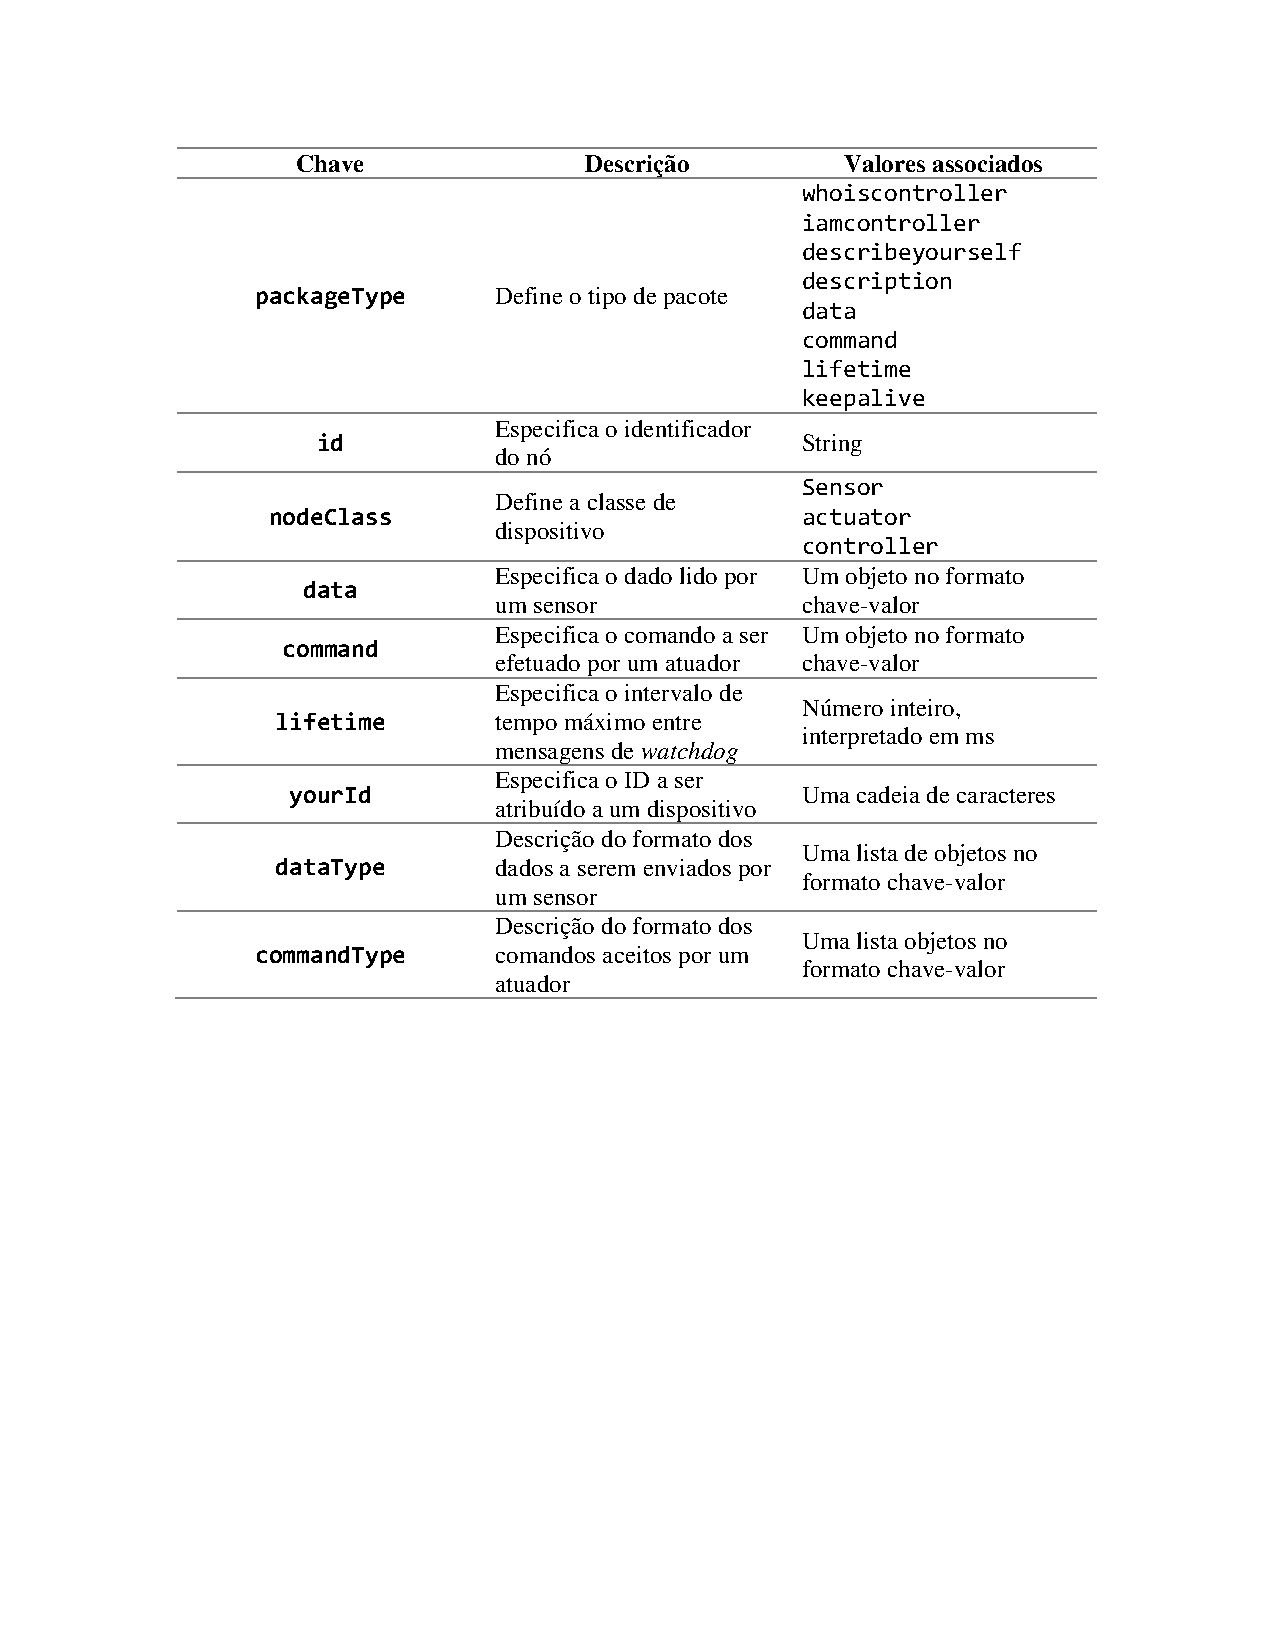
\includegraphics[width=0.9\textwidth]{tabelas/chave_valor_prot.pdf}
\end{table}

A chave \texttt{packageType} descreve o tipo do pacote, definindo os demais campos que devem estar presentes nele e como devem ser interpretados. Os poss�veis valores dessa chave s�o:

\paragraph*{\texttt{whoiscontroller}.} Esta mensagem � enviada por um dispositivo sensor ou atuador  por broadcast para descobrir o endere�o do controlador. 

\paragraph*{\texttt{iamcontroller}.} Mensagem enviada em resposta ao pedido de descoberta de controlador. Espera-se que este pacote conte com o seguinte campo:
\begin{itemize}
	\item \texttt{yourId}: esta mensagem � emitida pelo controlador, definindo o identificador a ser utilizado pelos dispositivos da rede nas comunica��es subsequentes.
\end{itemize}

\paragraph*{\texttt{describeyourself}.} Mensagem enviada pelo controlador solicitando ao dispositivo-alvo uma descri��o de suas funcionalidades.

\paragraph*{\texttt{description}.} Consiste na descri��o das funcionalidades do dispositivo, enviada em resposta ao pedido \texttt{describeyourself}. Espera-se que um pacote deste tipo conte com os seguintes campos:
\begin{itemize}
	\item \texttt{nodeClass}: define a classe de um dispositivo, que pode ser sensor, atuador ou controlador. Um sensor � definido como um dispositivo que envia dados de leitura. Um controlador � um dispositivo que recebe comandos e efetua a��es baseadas neles. Um controlador � um dispositivo que coordena sensores e atuadores, recebendo dados de leitura e enviando comandos de atua��o;
	\item \texttt{dataType}: especifica as classes de dados que s�o emitidos pelo sensor. Consiste em um objeto com chaves e valores definidos conforme mostra a Tabela \ref{tab:datatype}. O campo \texttt{category} define a categoria de dados coletados pelo sensor, al�m de especificar os tipos que podem ser alocados no campo \texttt{type}. A Tabela \ref{tab:classesdados} define os valores poss�veis de serem utilizados como categoria, al�m de listar os tipos de dados permitidos para cada categoria;
	\item \texttt{commandType}: especifica as classes de comandos aceitos pelo atuador. Consiste em um objeto com chaves e valores definidos conforme mostra a Tabela \ref{tab:commandtype}. O campo \texttt{category} define a categoria de comandos aceitos pelo atuador, al�m de especificar os tipos que podem ser alocados no campo \texttt{type}. A Tabela \ref{tab:classescomandos} define os valores poss�veis de serem utilizados como categoria, al�m de listar os tipos de dados permitidos para cada categoria.
\end{itemize}

\begin{table}[hp]
	\centering
	\caption{Chaves e valores associados utilizados na declara��o de tipos de dados lidos por um sensor.}\smallskip
	\label{tab:datatype}
	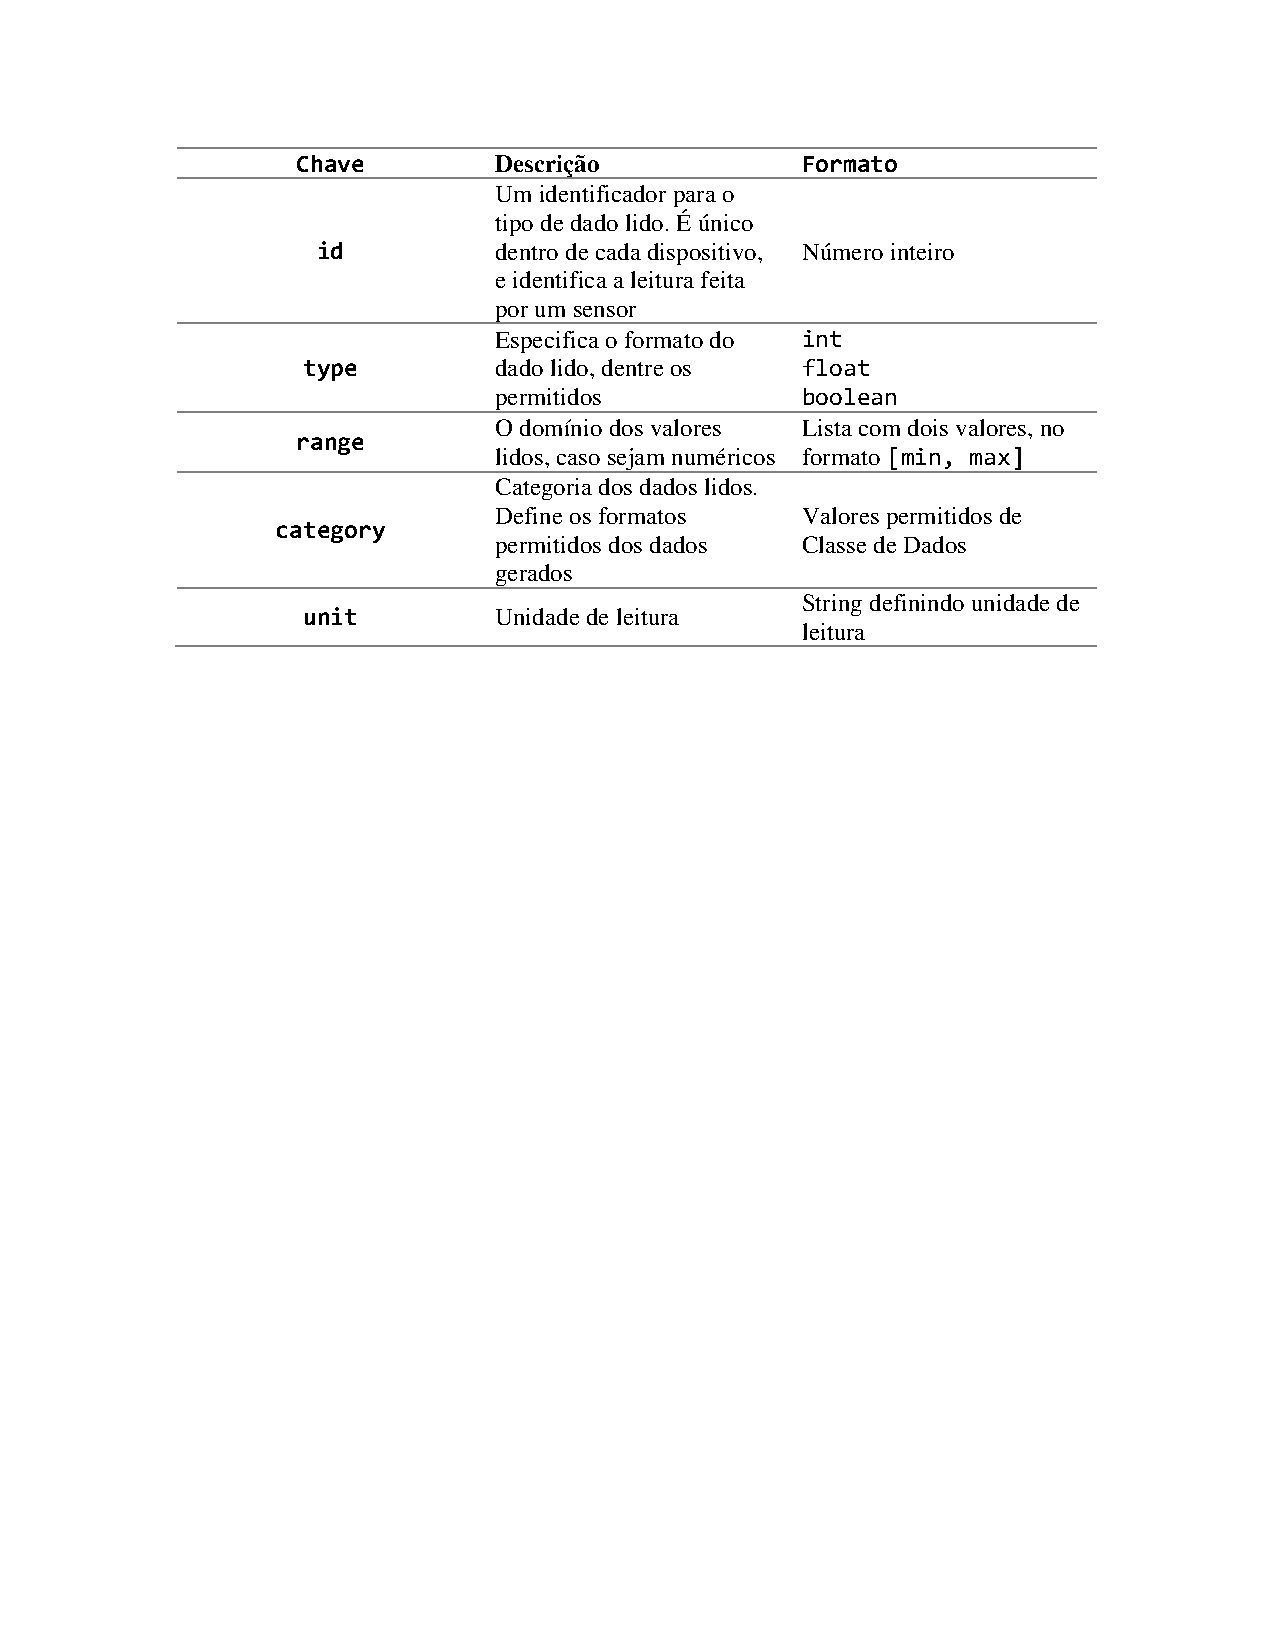
\includegraphics[width=0.9\textwidth]{tabelas/datatype.pdf}
	
	\medskip
	
	\caption{Categorias de dados e os respectivos tipos de valores permitidos.}\smallskip
	\label{tab:classesdados}
	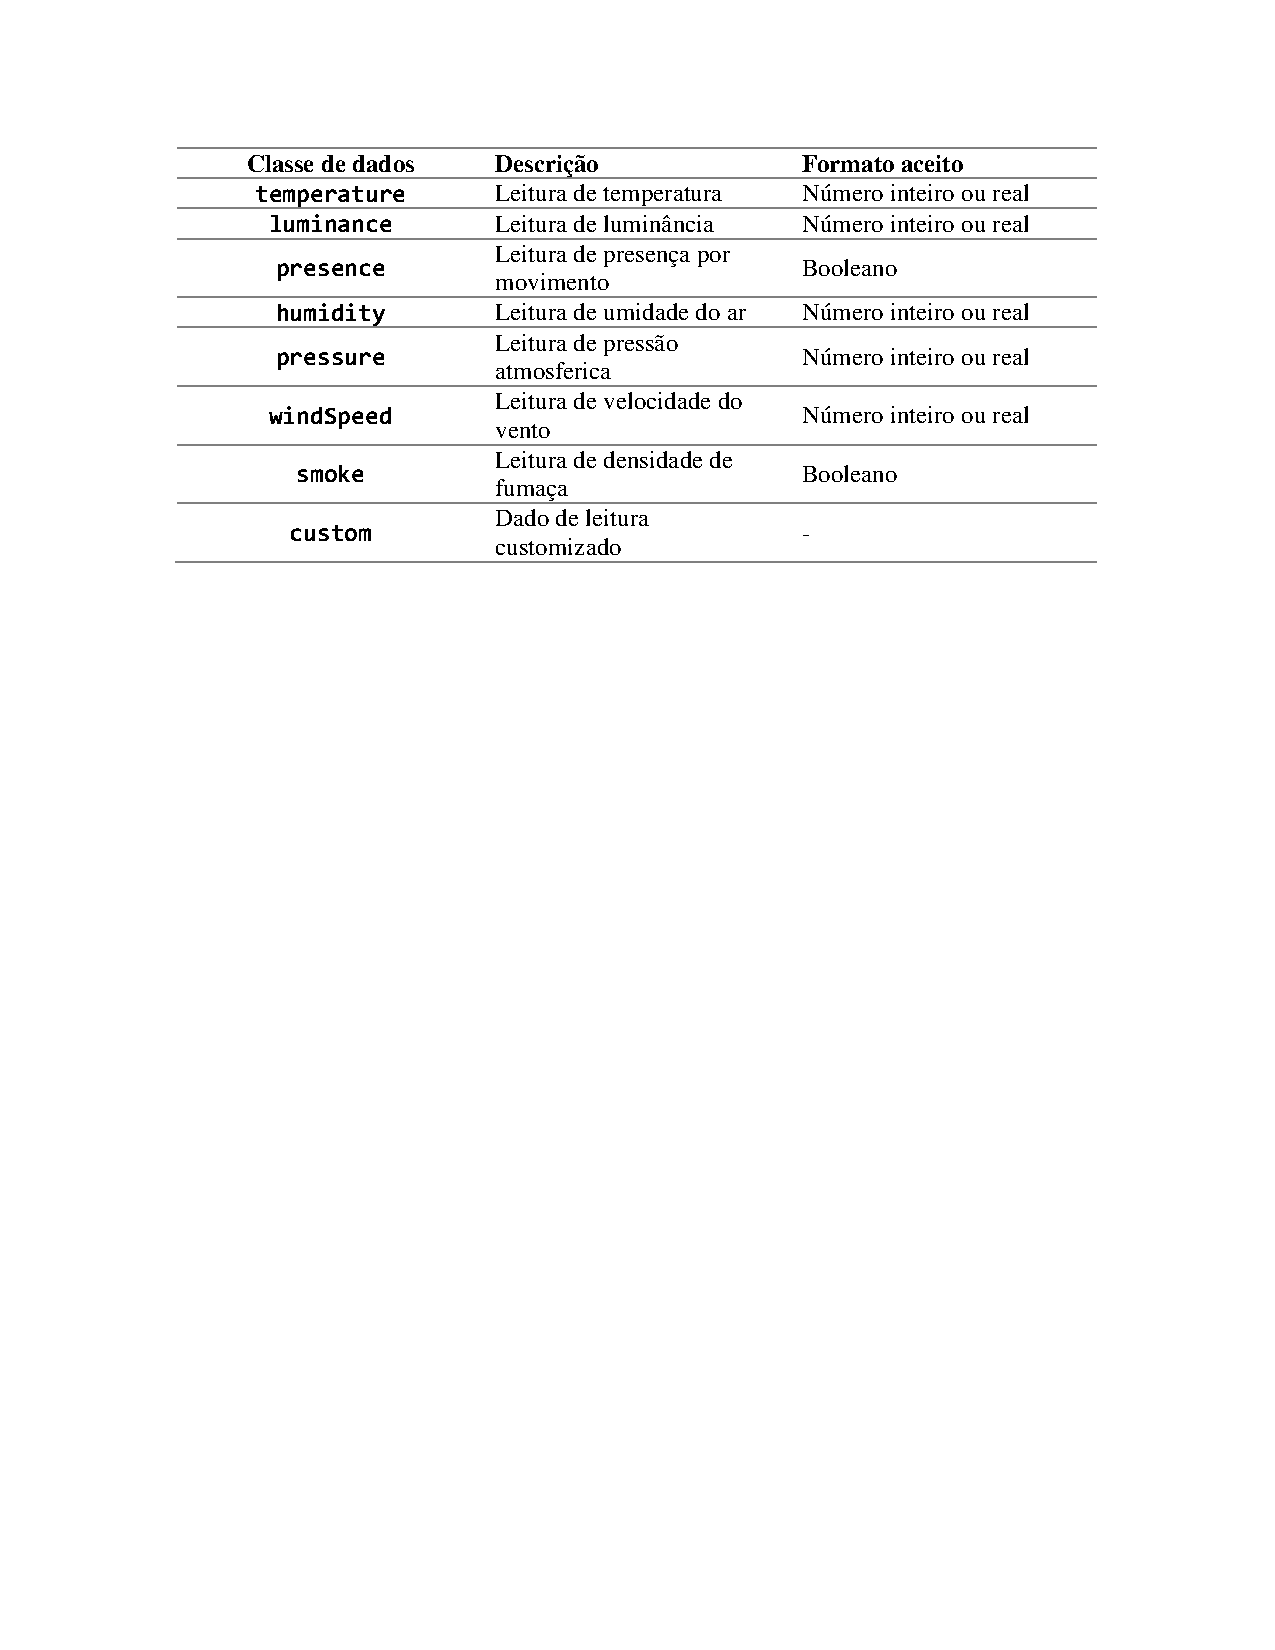
\includegraphics[width=0.9\textwidth]{tabelas/classes_dados.pdf}
\end{table}

\begin{table}[hp]
	\centering
	\caption{Chaves e valores associados utilizados na declara��o de tipos de comandos aceitos por um atuador.}\smallskip
	\label{tab:commandtype}
	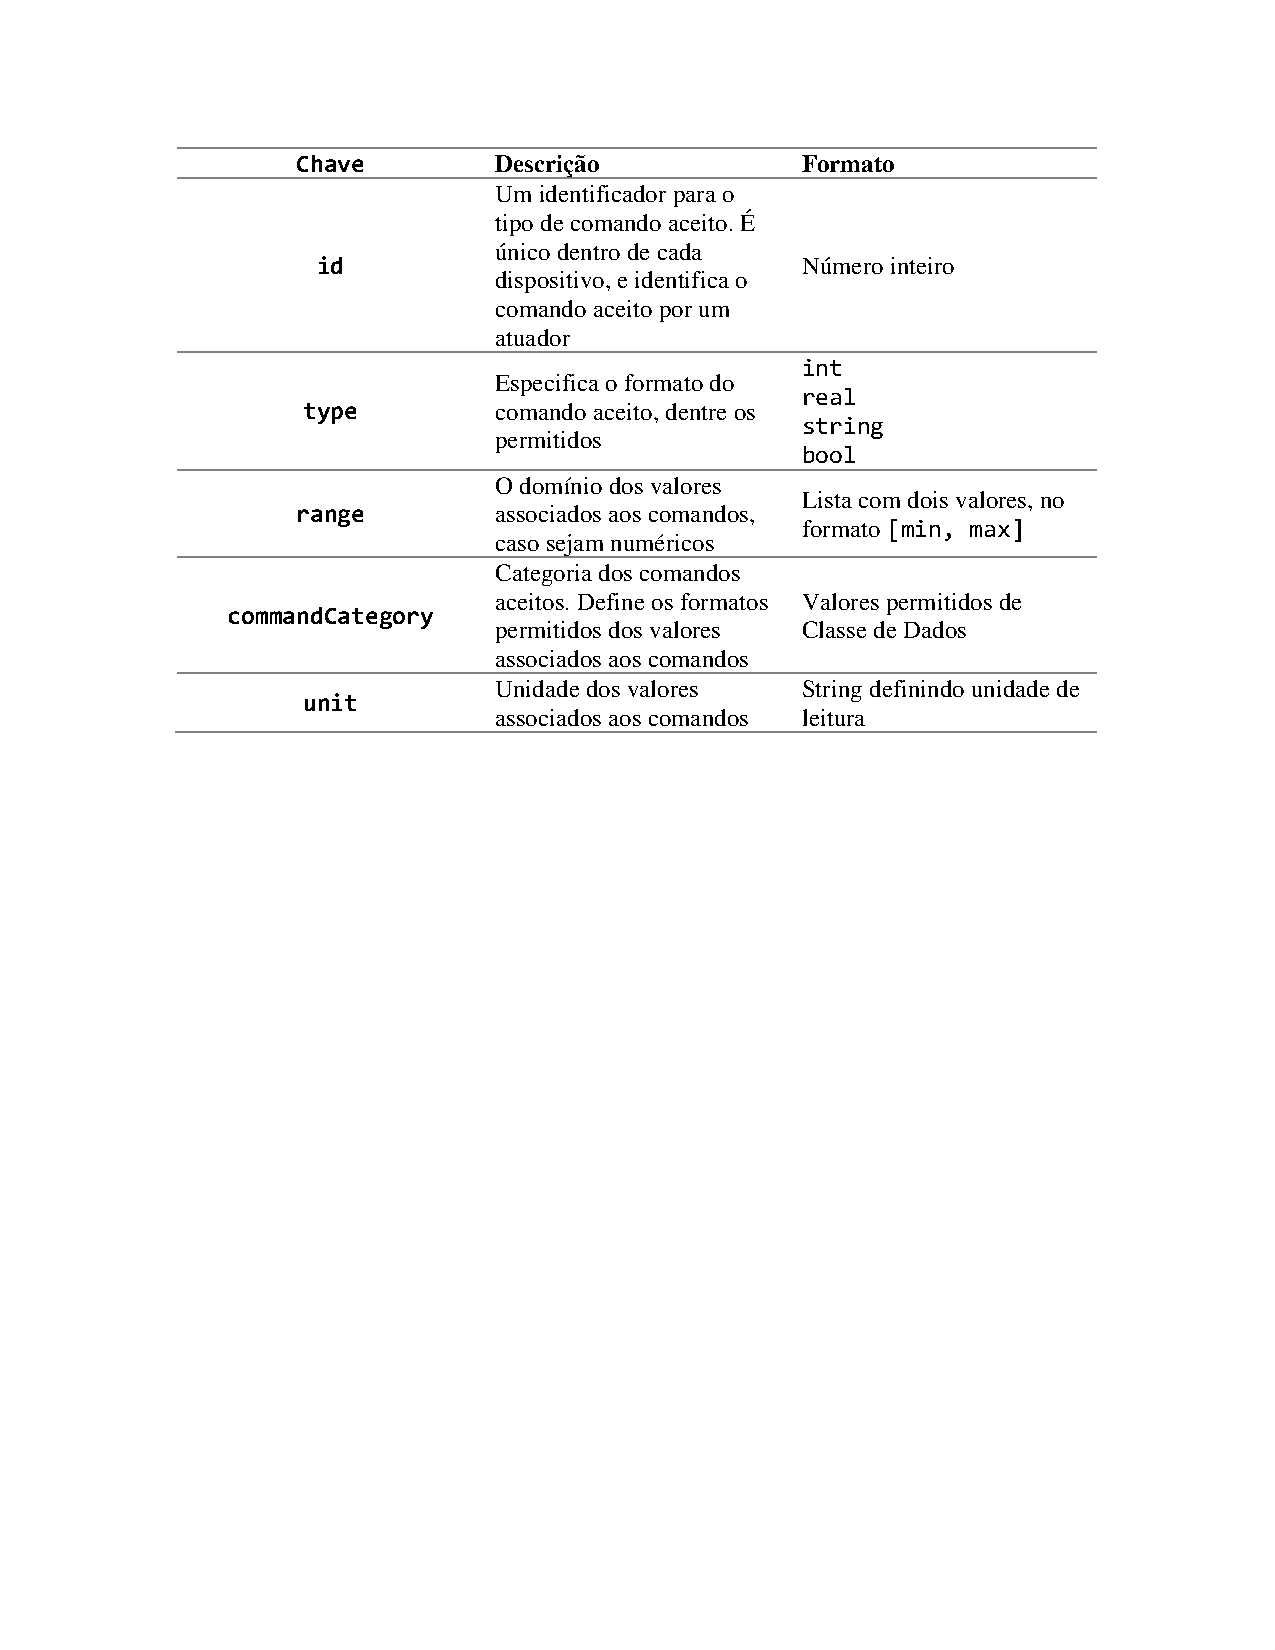
\includegraphics[width=0.9\textwidth]{tabelas/commandtype.pdf}
	
	\medskip
	
	\caption{Categorias de comandos e os respectivos tipos de valores permitidos.}\smallskip
	\label{tab:classescomandos}
	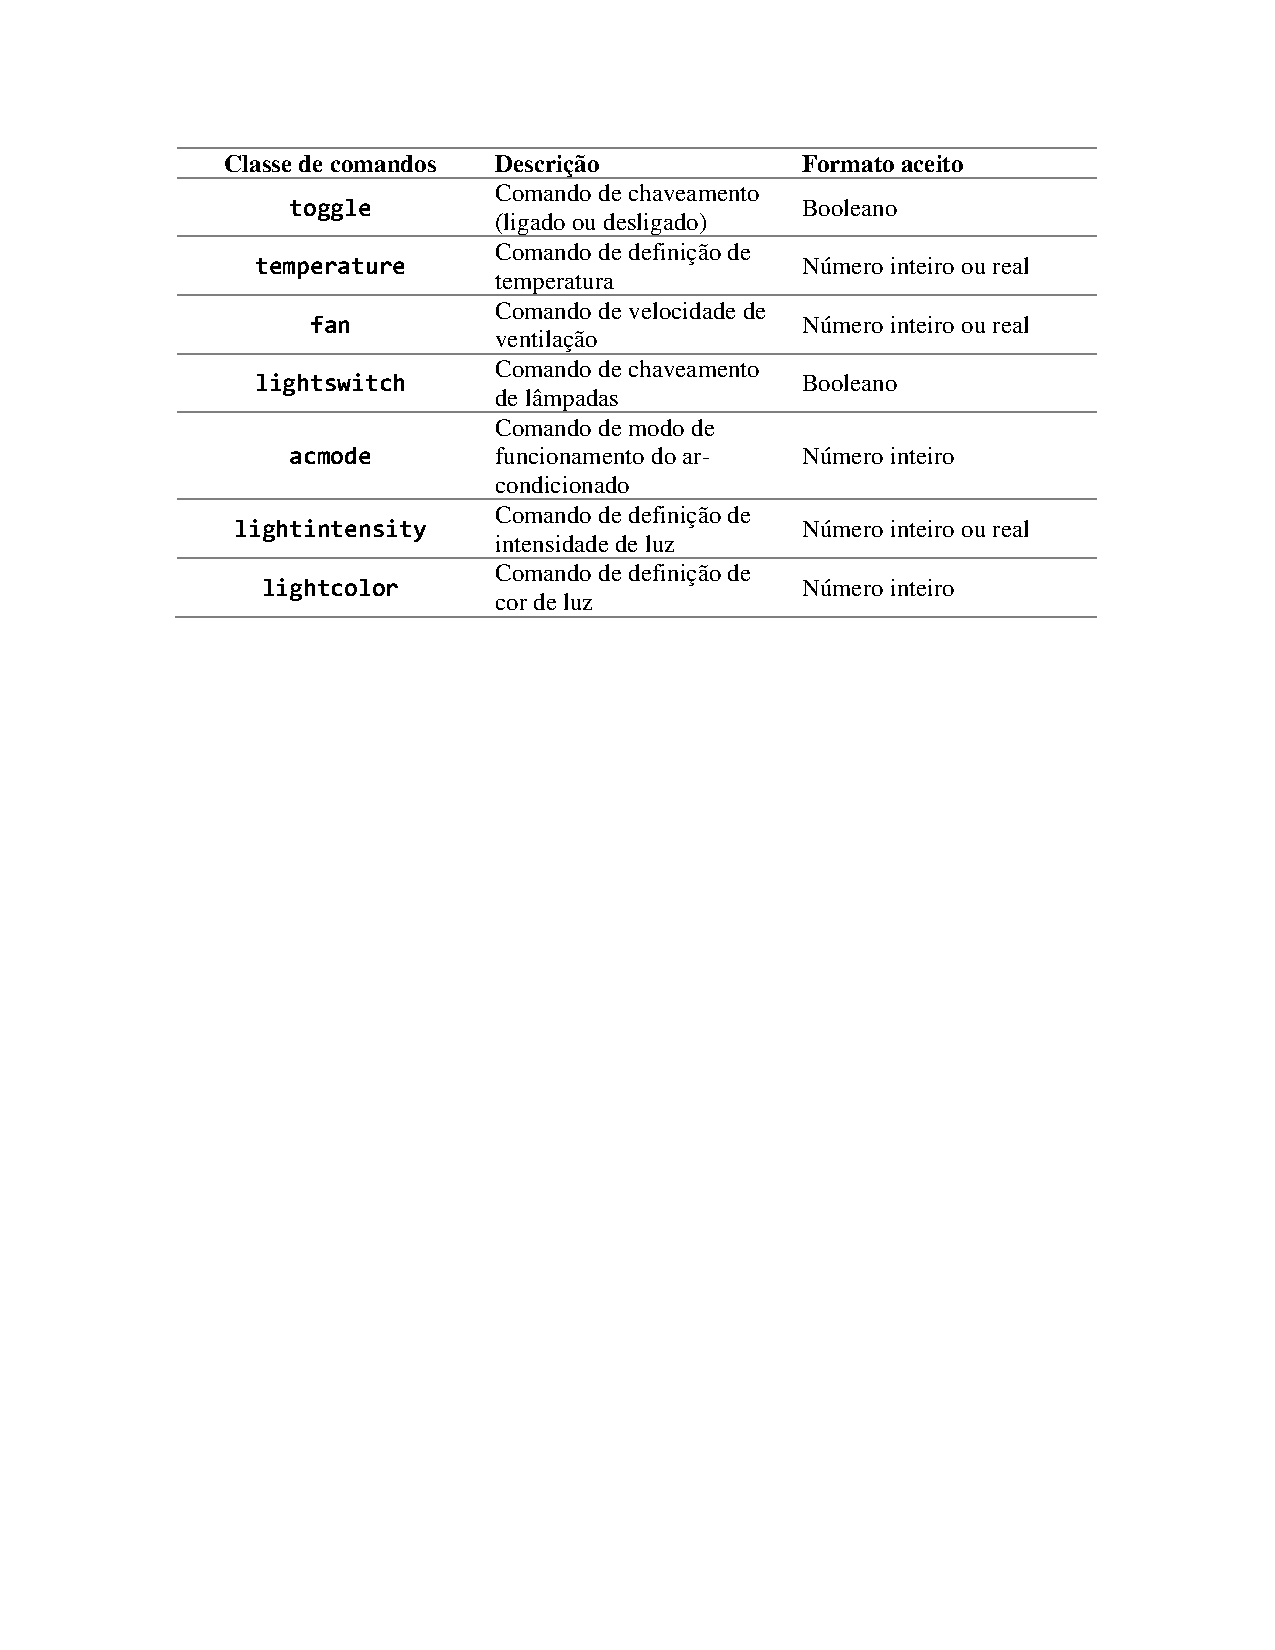
\includegraphics[width=0.9\textwidth]{tabelas/classes_comandos.pdf}
\end{table}

\paragraph*{\texttt{data}.} Descreve uma mensagem contendo dados de leitura de um sensor. Espera-se que um pacote deste tipo conte com o seguinte campo:
\begin{itemize}
	\item \texttt{data}: especifica o dado lido por um sensor. Possui como valor associado um objeto com os campos listados na Tabela \ref{tab:chaves_dado}.
\end{itemize}

\begin{table}[h]
	\centering
	\caption{Chaves e valores associados utilizados na transmiss�o de um dado por um sensor.}\smallskip
	\label{tab:chaves_dado}
	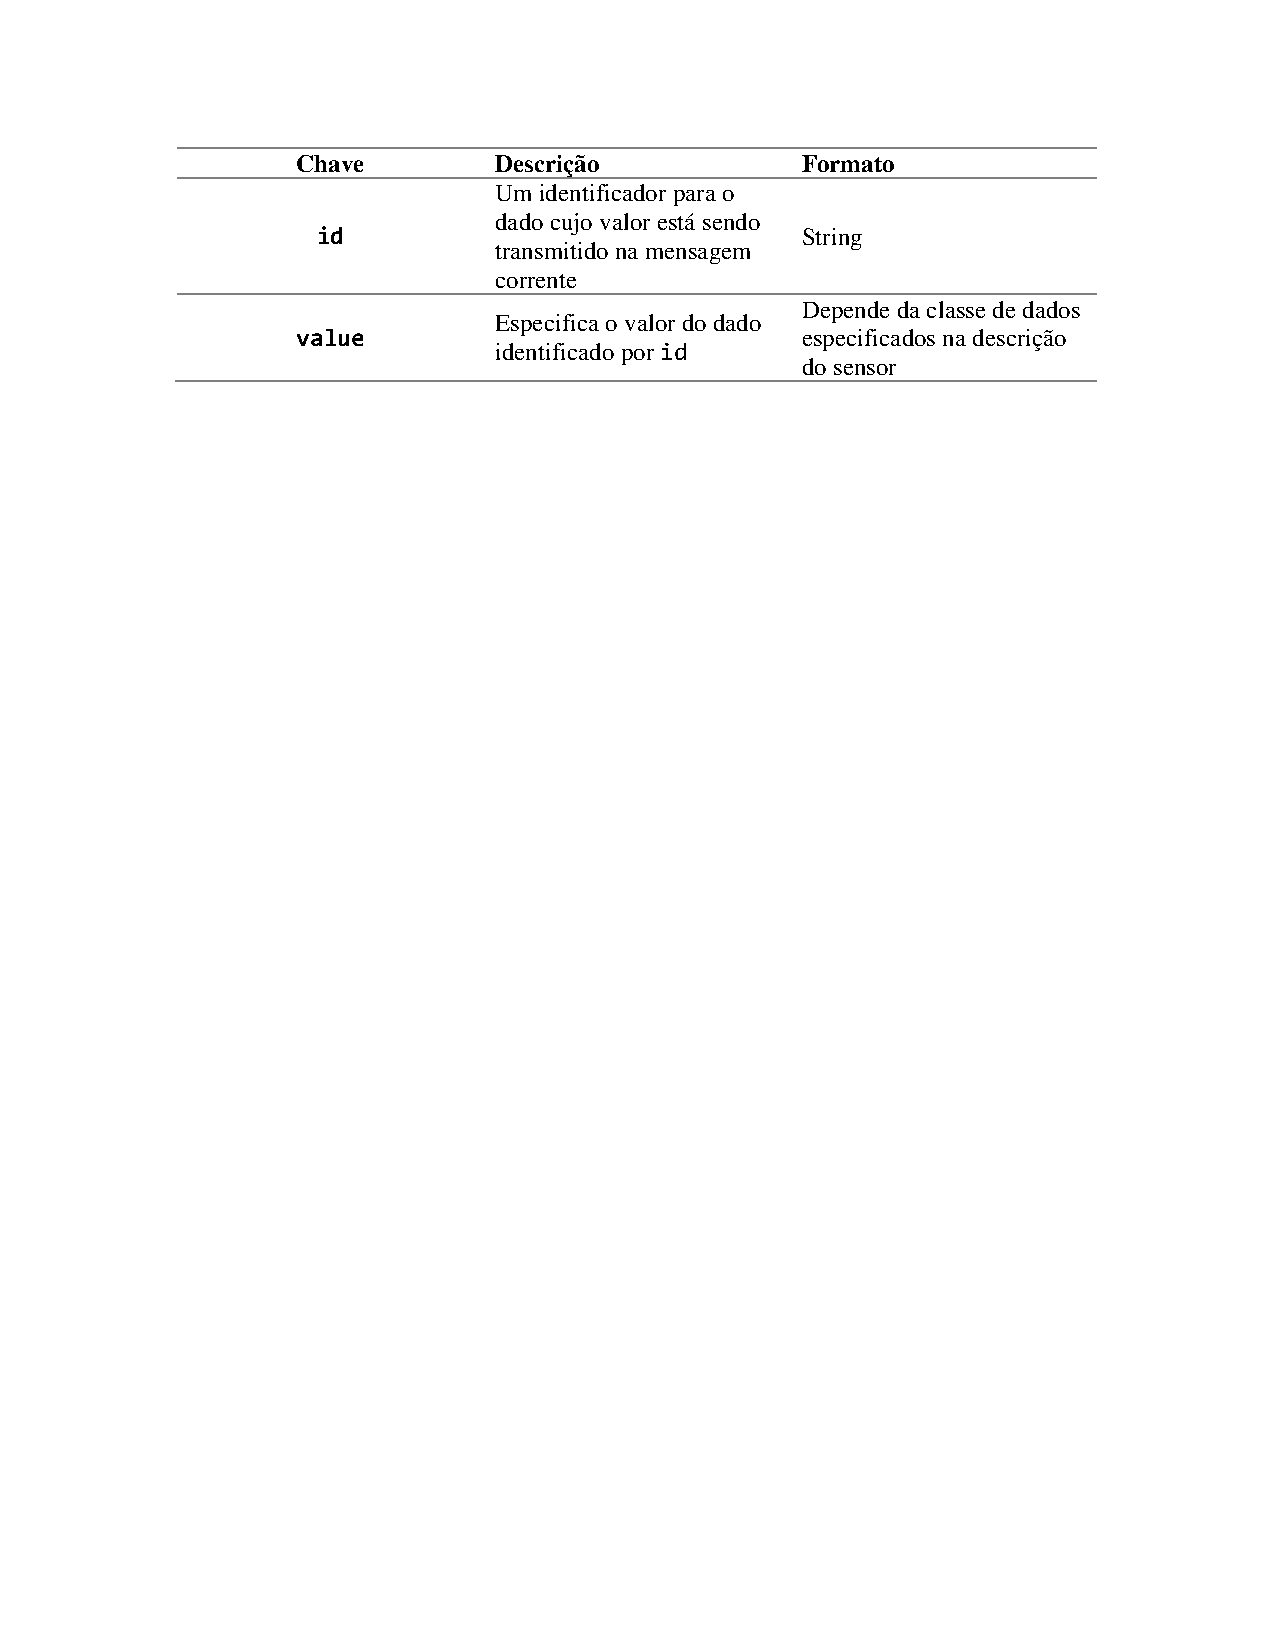
\includegraphics[width=0.9\textwidth]{tabelas/chaves_dado.pdf}
\end{table}

\paragraph*{\texttt{command}.} Descreve uma mensagem contendo comandos destinados a um atuador. Espera-se que um pacote deste tipo conte com o seguinte campo:
\begin{itemize}
	\item \texttt{command} especifica o comando destinado a um atuador. Possui como valor associado um objeto com os campos listados na Tabela \ref{tab:chaves_comando}.
\end{itemize}

\begin{table}[h]
	\centering
	\caption{Chaves e valores associados utilizados na transmiss�o de um comando para um atuador.}\smallskip
	\label{tab:chaves_comando}
	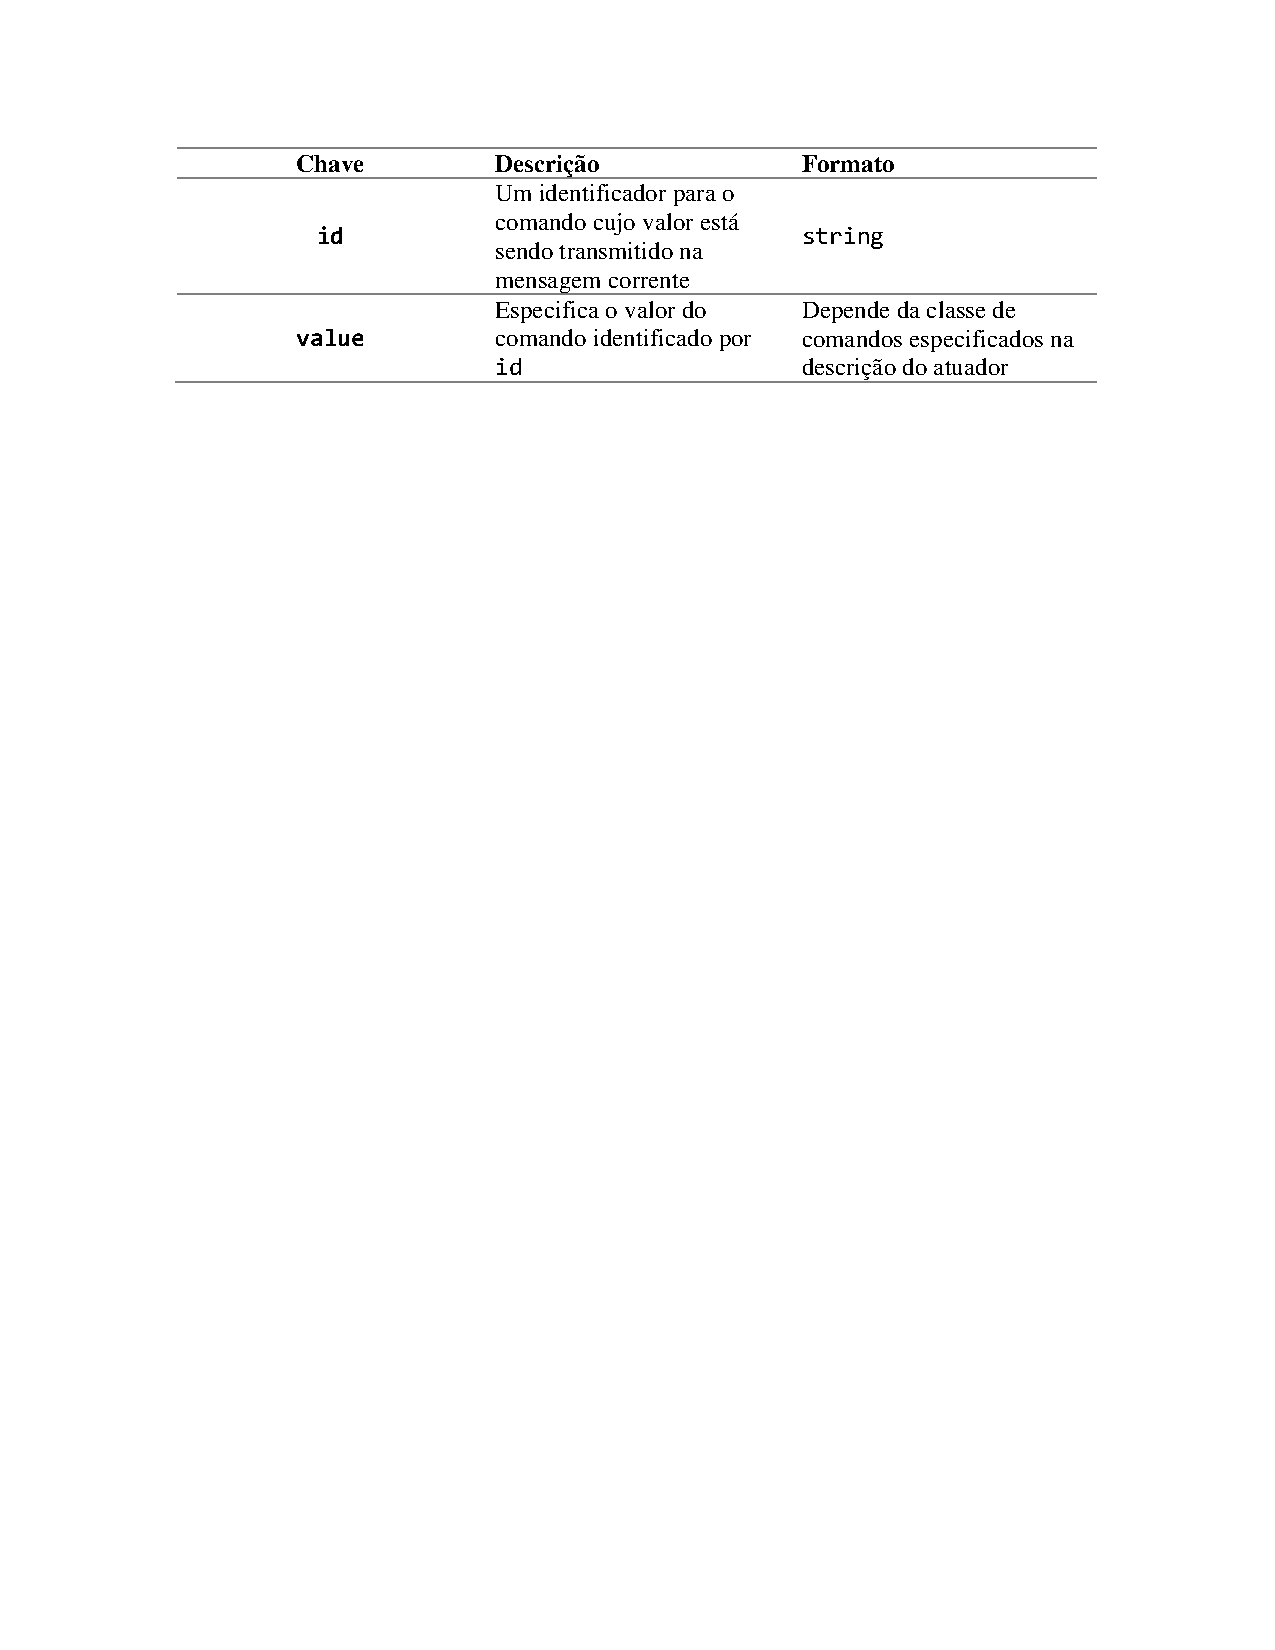
\includegraphics[width=0.9\textwidth]{tabelas/chaves_comando.pdf}
\end{table}

\paragraph*{\texttt{lifetime}.} Mensagem especificando o intervalo m�ximo de envio de sinais de  \textit{heartbeat}. Espera-se que uma mensagem deste tipo conte com o seguinte campo:
\begin{itemize}
	\item \texttt{lifetime}: especifica o intervalo de tempo m�ximo entre mensagens de \textit{heartbeat}. Esta mensagem � emitida pelo controlador aos dispositivos, regulando a frequ�ncia de envio de mensagens do tipo \texttt{keepalive}.
\end{itemize}

\paragraph*{\texttt{keepalive}.} Especifica uma mensagem que deve ser interpretada como sinal de  \textit{heartbeat}.

\paragraph*{\texttt{iamback}.} Emitida por um sensor ou atuador caso ele tenha recebido um identificador anteriormente, mas devido a alguma raz�o, foi desconectado da rede e necessita se reconectar.

\paragraph*{\texttt{welcomeback}.} Mensagem emitida por um controlador ao receber uma mensagem do tipo \texttt{iamback}, indicando que o dispositivo foi reconhecido e aceito na rede.

\paragraph*{\texttt{externalcommand}.} Mensagem emitida por um dispositivo atuador, indicando que um comando de origem externa ao sistema foi recebido. A estrutura desta mensagem � igual �s do tipo \texttt{command}.

Cabe apontar que as mensagens dos tipos \texttt{description}, \texttt{data}, \texttt{command}, \texttt{keepalive}, \texttt{iamback} e \texttt{externalcommand} devem possuir o campo \texttt{id}, que identifica o dispositivo.

Note, ainda, que chaves do tipo \texttt{packageType} e \texttt{nodeClass} podem ter m�ltiplos valores associados. Por exemplo, uma mensagem pode ser enviada com os tipos \texttt{iamcontroller}, \texttt{describeyourself} e \texttt{lifetime}, indicando que ela tem as fun��es de identificar o controlador, solicitar informa��es ao dispositivo-destino e definir o intervalo de envio de sinais de \textit{heartbeat}.

\subsection{Protocolo de Troca de Mensagens}
Definida a estrutura do pacote, suas chaves e seus valores associados, pode-se passar para a defini��o do aspecto din�mico do protocolo. Esta se��o busca definir o sequenciamento de mensagens para efetuar a��es espec�ficas na rede de sensores.

\paragraph*{Inicializa��o.} O processo de inicializa��o dos sensores est� esquematizado na Figura \ref{fig:uml_handshake}. Assim que um dispositivo � conectado � rede, ele emite um pacote do tipo \texttt{whiiscontroller} em broadcast, com o objetivo de descobrir o endere�o do controlador, caso exista. Em seguida, o controlador responde com uma mensagem do tipo \texttt{iamcontroller} ao dispositivo solicitante, permitindo que ele identifique o endere�o do coordenador. Al�m disso, nesta mensagem, o controlador define o identificador do dispositivo.

Em seguida, o controlador solicita uma descri��o do dispositivo com um pacote do tipo \texttt{describeyourself}, � qual o dispositivo responde com uma mensagem \texttt{description}. Ela cont�m informa��es como a classe do n�, tipos de dados gerados (caso seja sensor) e tipos de comandos aceitos (caso seja atuador).

O controlador tamb�m pode definir um intervalo m�ximo em que o dispositivo deve enviar mensagens de \textit{heartbeat} atrav�s do pacote \texttt{lifetime}. O dispositivo, neste caso, envia pacotes \textit{heartbeat} periodicamente, sinalizando os pacotes como sendo do tipo \texttt{keepalive}.

\begin{figure}[h]
	\centering

	\caption{Processo de inicializa��o de um dispositivo.} 
	\medskip
  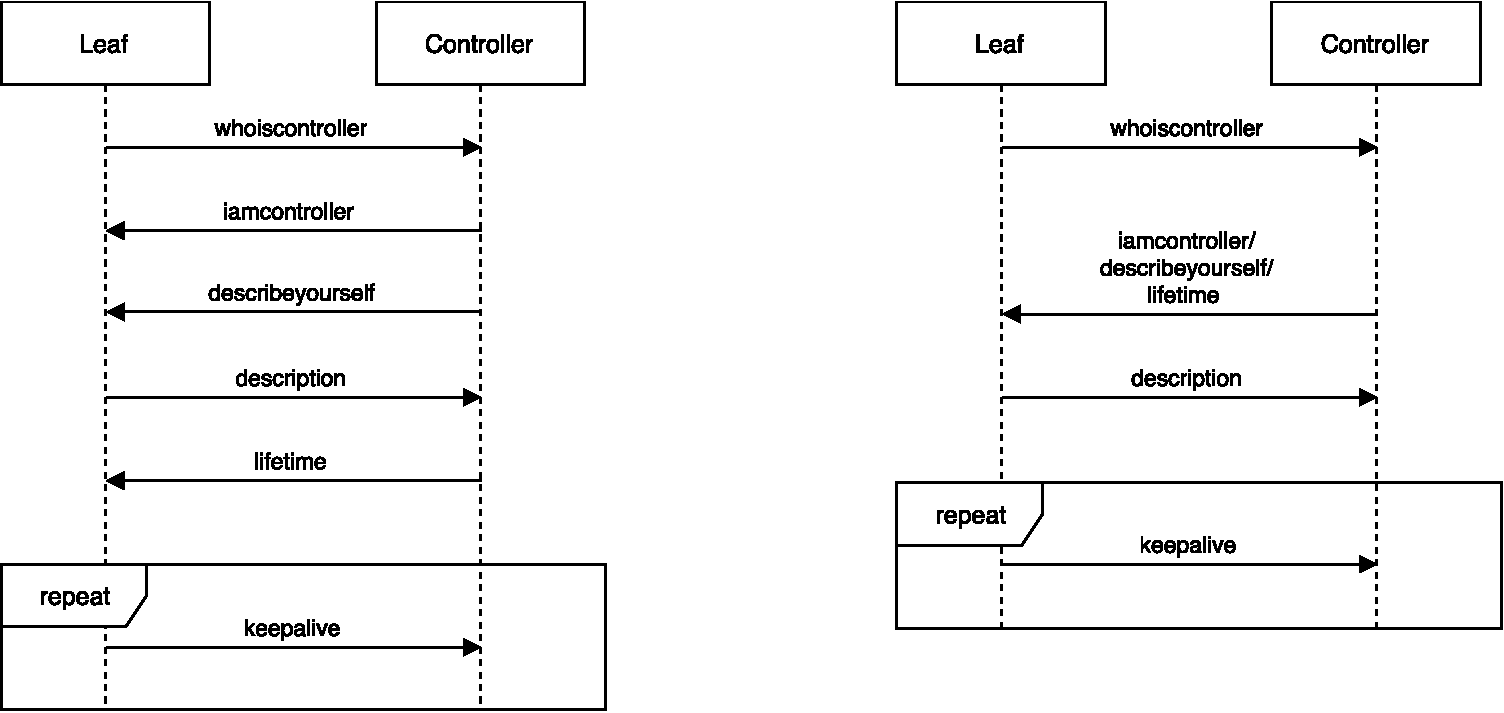
\includegraphics[width=\textwidth]{imagens/uml_handshake.pdf}
  \label{fig:uml_handshake}
\end{figure}

O processo de inicializa��o pode ser simplificado condensando-se os pacotes \texttt{iamcontroller}, \texttt{describeyourself} e \texttt{lifetime} (caso aplic�vel) em um �nico pacote, conforme ilustra o diagrama � direita da Figura \ref{fig:uml_handshake}.

\paragraph*{Envio de dados.} Uma vez efetuado o processo de inicializa��o, dados de leitura podem ser enviados do sensor ao controlador atrav�s da mensagem \texttt{data}.

\paragraph*{Envio de comandos.} Uma vez efetuado o processo de inicializa��o, comandos podem ser enviados do controlador ao atuador atrav�s da mensagem \texttt{command}.

\paragraph*{Retorno � rede.} Caso um dispositivo operante se desconecte da rede por algum motivo, ele pode se reconectar enviando uma mensagem do tipo \texttt{imback}, conforme ilustra a Figura \ref{fig:uml_reconnect}. Ao receber uma mensagem deste tipo, o controlador pode responder de duas maneiras. Caso ele reconhe�a o identificador enviado pelo dispositivo na mensagem \texttt{imback}, ele responde com outra mensagem do tipo \texttt{welcomeback}, conforme ilustra o diagrama � esquerda da Figura \ref{fig:uml_reconnect}. A partir deste momento, o dispositivo pode operar regularmente. Por outro lado, caso o controlador n�o reconhe�a o dispositivo, ele solicita uma nova declara��o, como ilustrado no diagrama � direita da Figura \ref{fig:uml_reconnect}.

\begin{figure}[h]
	\centering
	\caption{Processo de retorno de um dispositivo � rede.}
	\medskip
  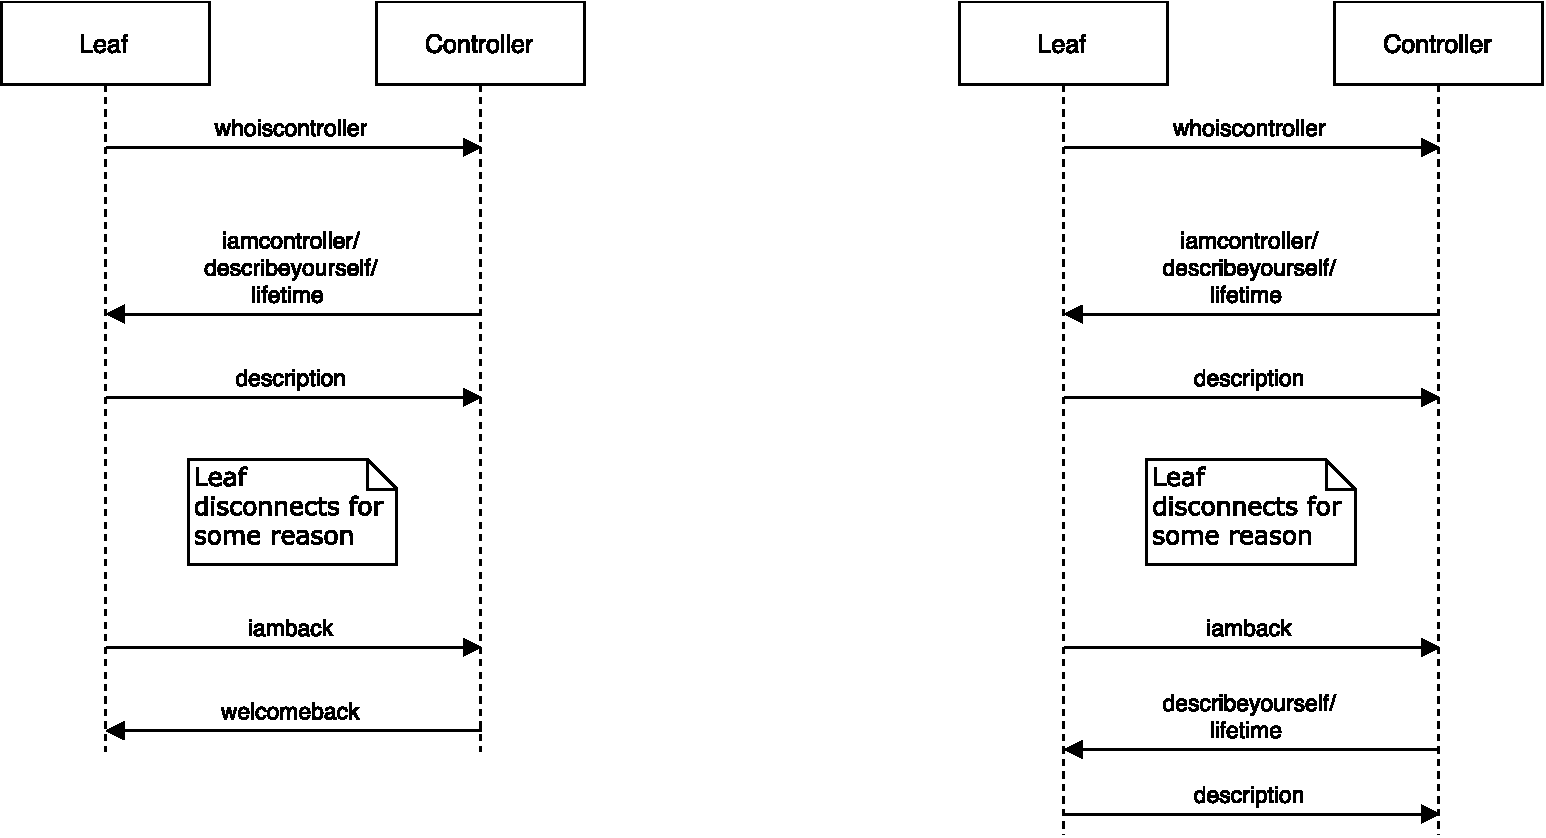
\includegraphics[width=\textwidth]{imagens/uml_reconnect.pdf}
  \label{fig:uml_reconnect}
\end{figure}

\subsection{A codifica��o CBOR}
Como mencionado, redes de sensores sem fio s�o compostas por dispositivos com limita��es de banda e de processamento. Por esta raz�o, � importante que as mensagens trafegadas sejam concisas (aliviando requisitos de banda) e de simples interpreta��o (aliviando requisitos de processamento). Com esses prop�sitos em mente, resolveu-se adotar a codifica��o CBOR (\textit{Concise Binary Object Representation}) \cite{rfc7049}.

Esta codifica��o � baseada no formato de dados JSON, provendo uma maneira de representar objetos neste formato de forma bin�ria. Sua especifica��o reconhece diversos tipos de dados, tais como inteiros negativos e n�o-negativos, cadeias de bytes e de caracteres, entre outros, cada qual com regras espec�ficas de representa��o. Para identificar o tipo de cada dado, a codifica��o dedica um byte para cada item de dado para descrev�-lo.

Considere como exemplo a codifica��o do objeto JSON a seguir:
\begin{center}
	\texttt{\{"a": 1, "b": 2\}}
\end{center}

Uma representa��o poss�vel do objeto acima pode ser feito em forma de cadeia de caracteres. Apresar de ser uma forma comum e pr�tica de se representar tais objetos, ela possui a desvantagem de ser extensa: no exemplo dado, considerando que um caractere ocupa 1 byte, o resultado gerado possui 13 bytes. Por outro lado, sua representa��o em CBOR ocupa 7 bytes, conforme apresentado na Tabela \ref{tab:cbor_exemplo}. Isso corresponde a uma redu��o de quase 50\% no resultado gerado.

\begin{table}[h]
	\centering
	\caption{Exemplo de representa��o em CBOR de um objeto JSON.}\smallskip
	\label{tab:cbor_exemplo}
	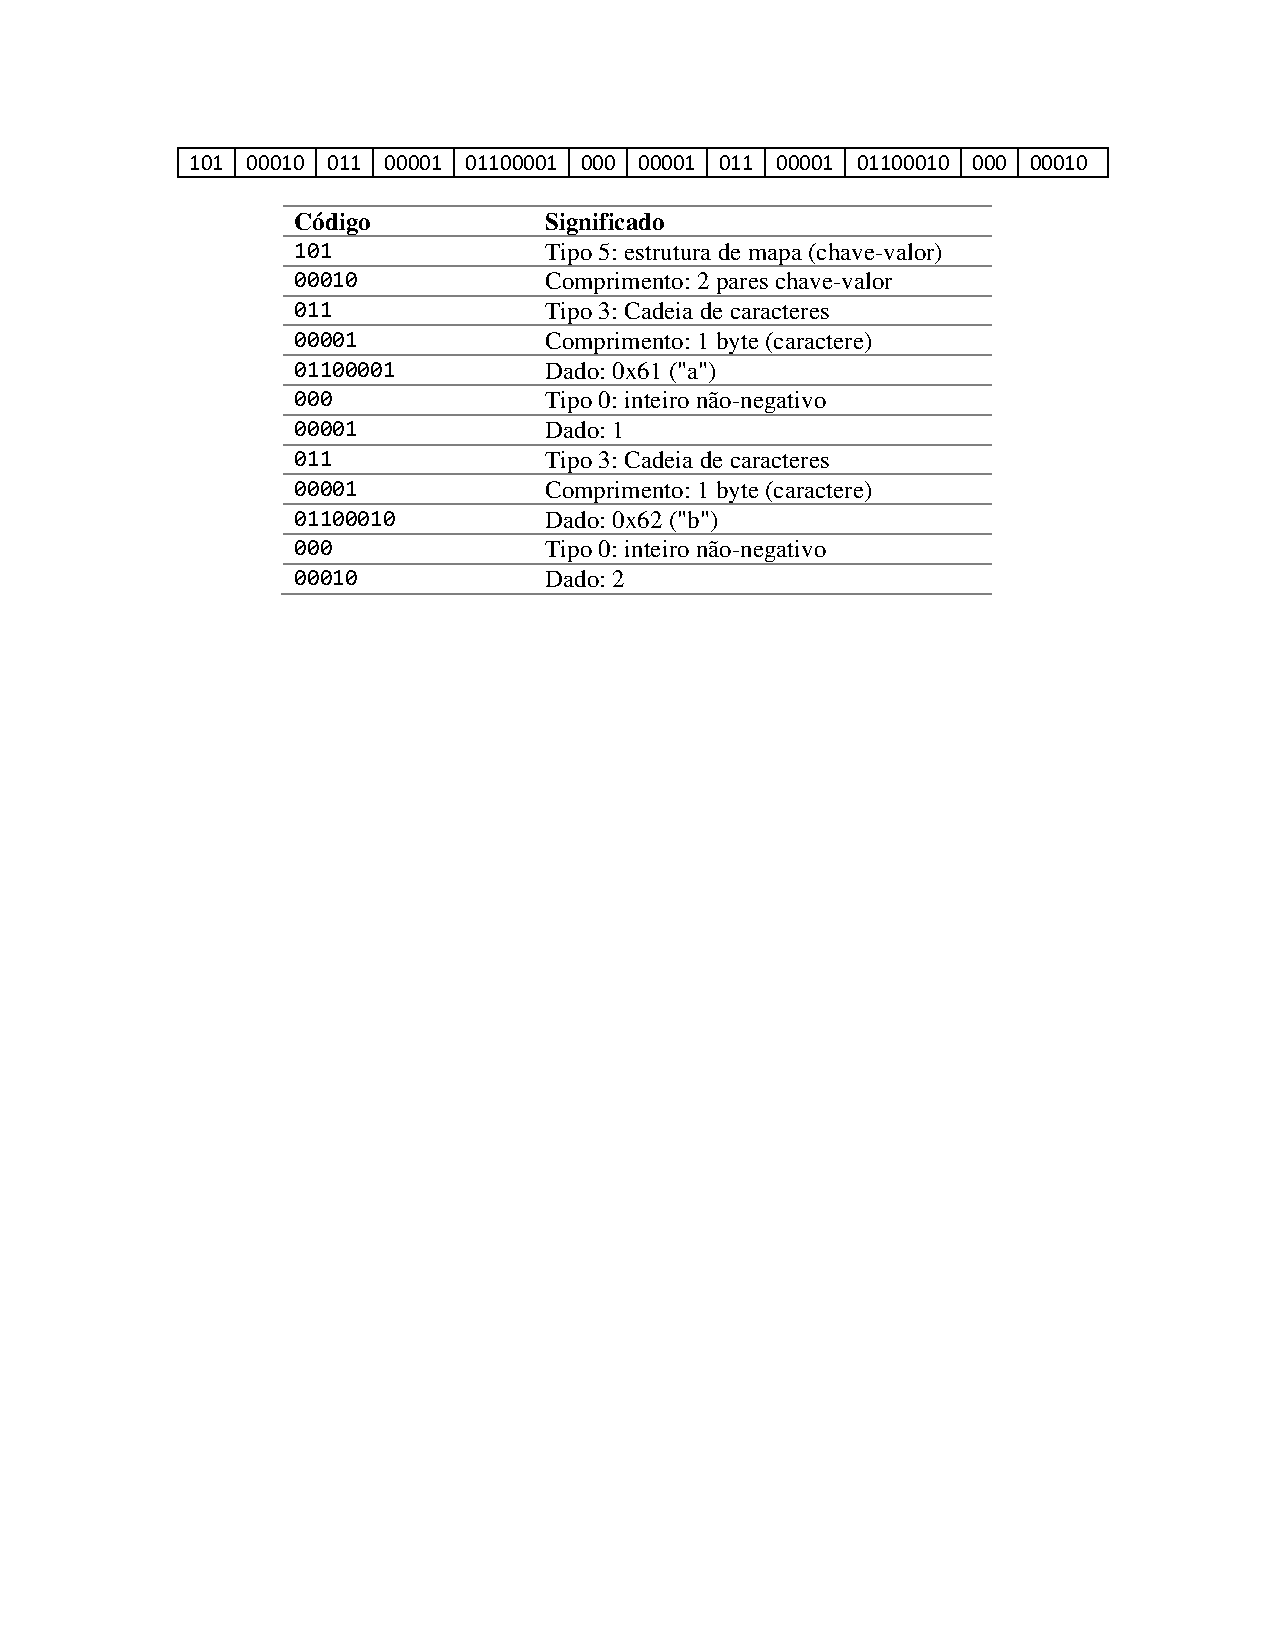
\includegraphics[width=0.9\textwidth]{tabelas/cbor_exemplo.pdf}
\end{table}

\subsection{Codifica��o dos Itens nas Mensagens}
Seguindo a ideia de manter concis�o nas mensagens trocadas, e levando em conta o funcionamento da codifica��o CBOR, os campos e valores especificados na se��o \ref{subsec:sintaxe} devem ser codificados antes da transmiss�o. As Tabelas \ref{tab:codificacao_chaves_principais}, \ref{tab:codificacao_tipo_dc} e \ref{tab:codificacao_dc} listam as codifica��es adotadas para as chaves das mensagens transmitidas.

\begin{table}[hp]
	\centering
	\caption{Codifica��o das chaves principais de uma mensagem.}\smallskip
	\label{tab:codificacao_chaves_principais}
	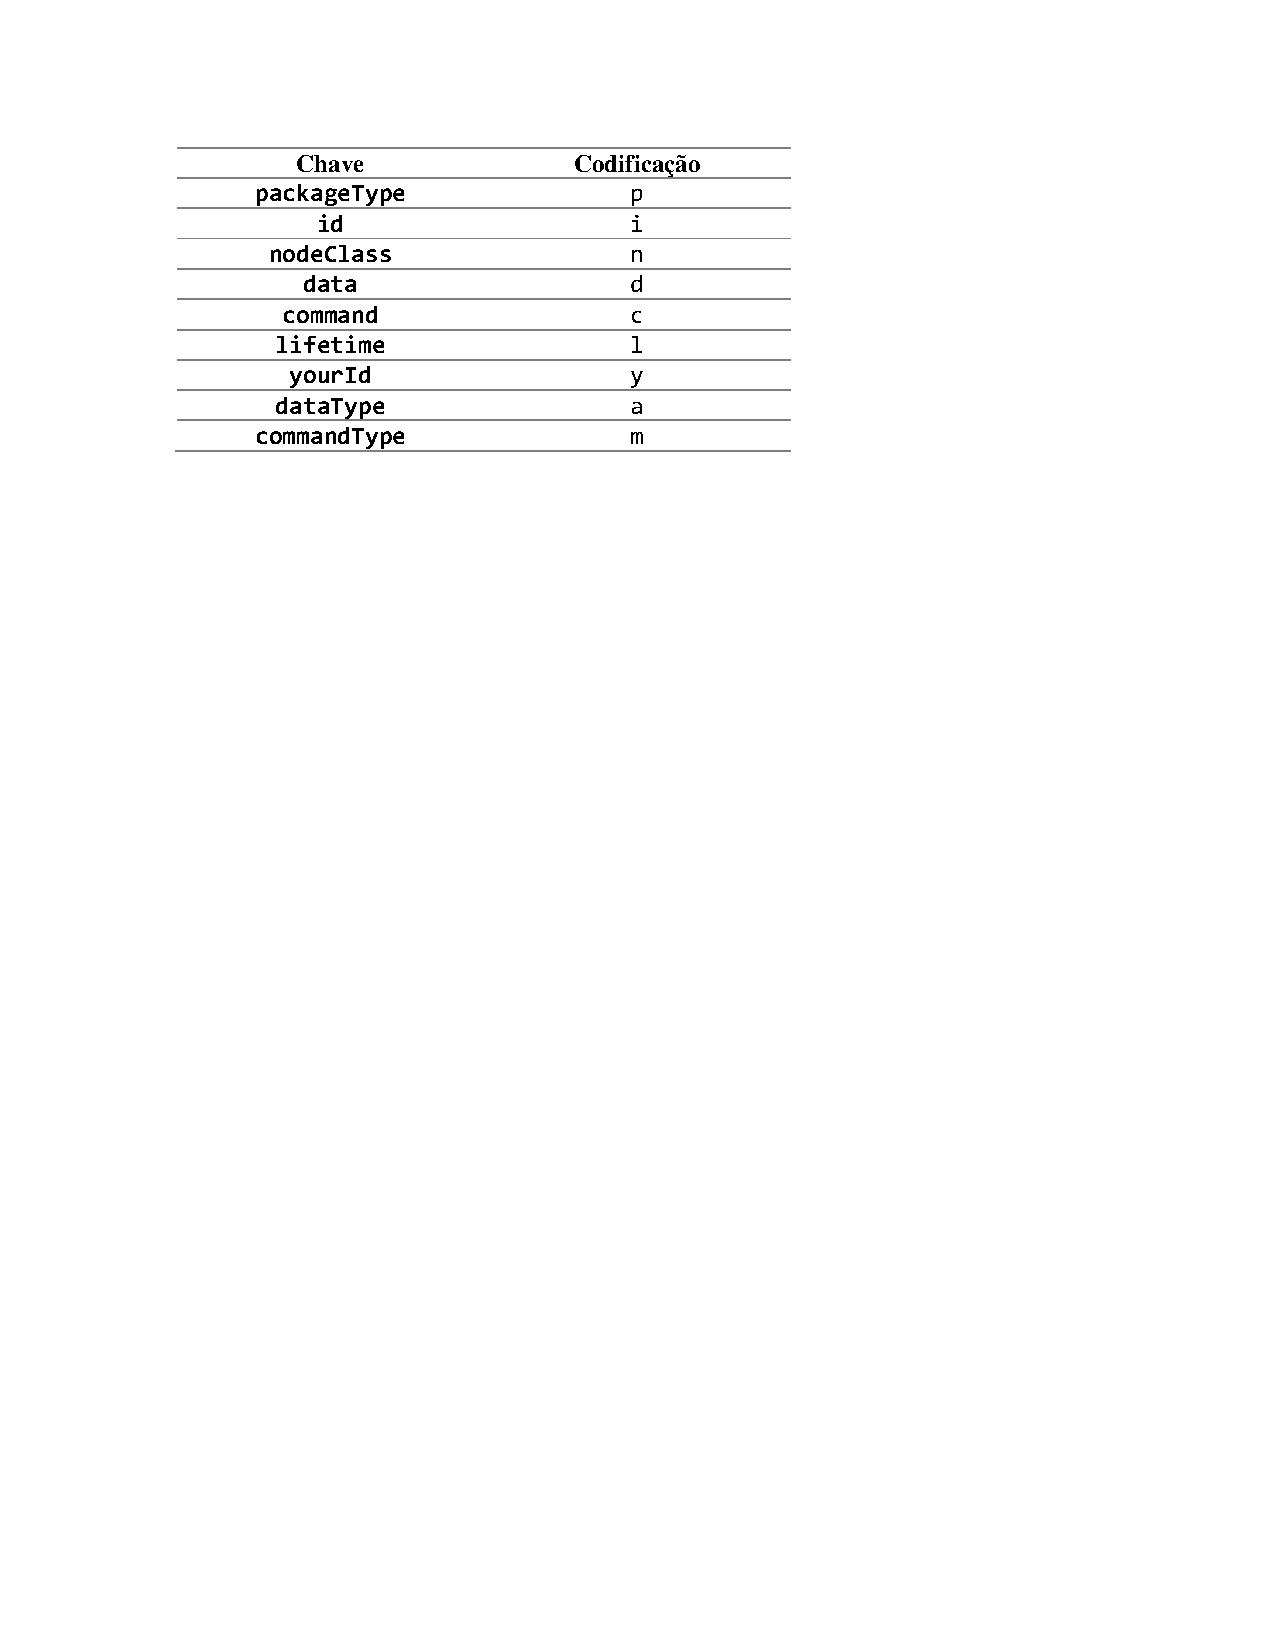
\includegraphics[width=0.7\textwidth]{tabelas/codificacao_chaves_principais.pdf}
	
	\caption{Codifica��o de chaves utilizadas nos campos \texttt{datatype} e \texttt{commandtype}.}\smallskip
	\label{tab:codificacao_tipo_dc}
	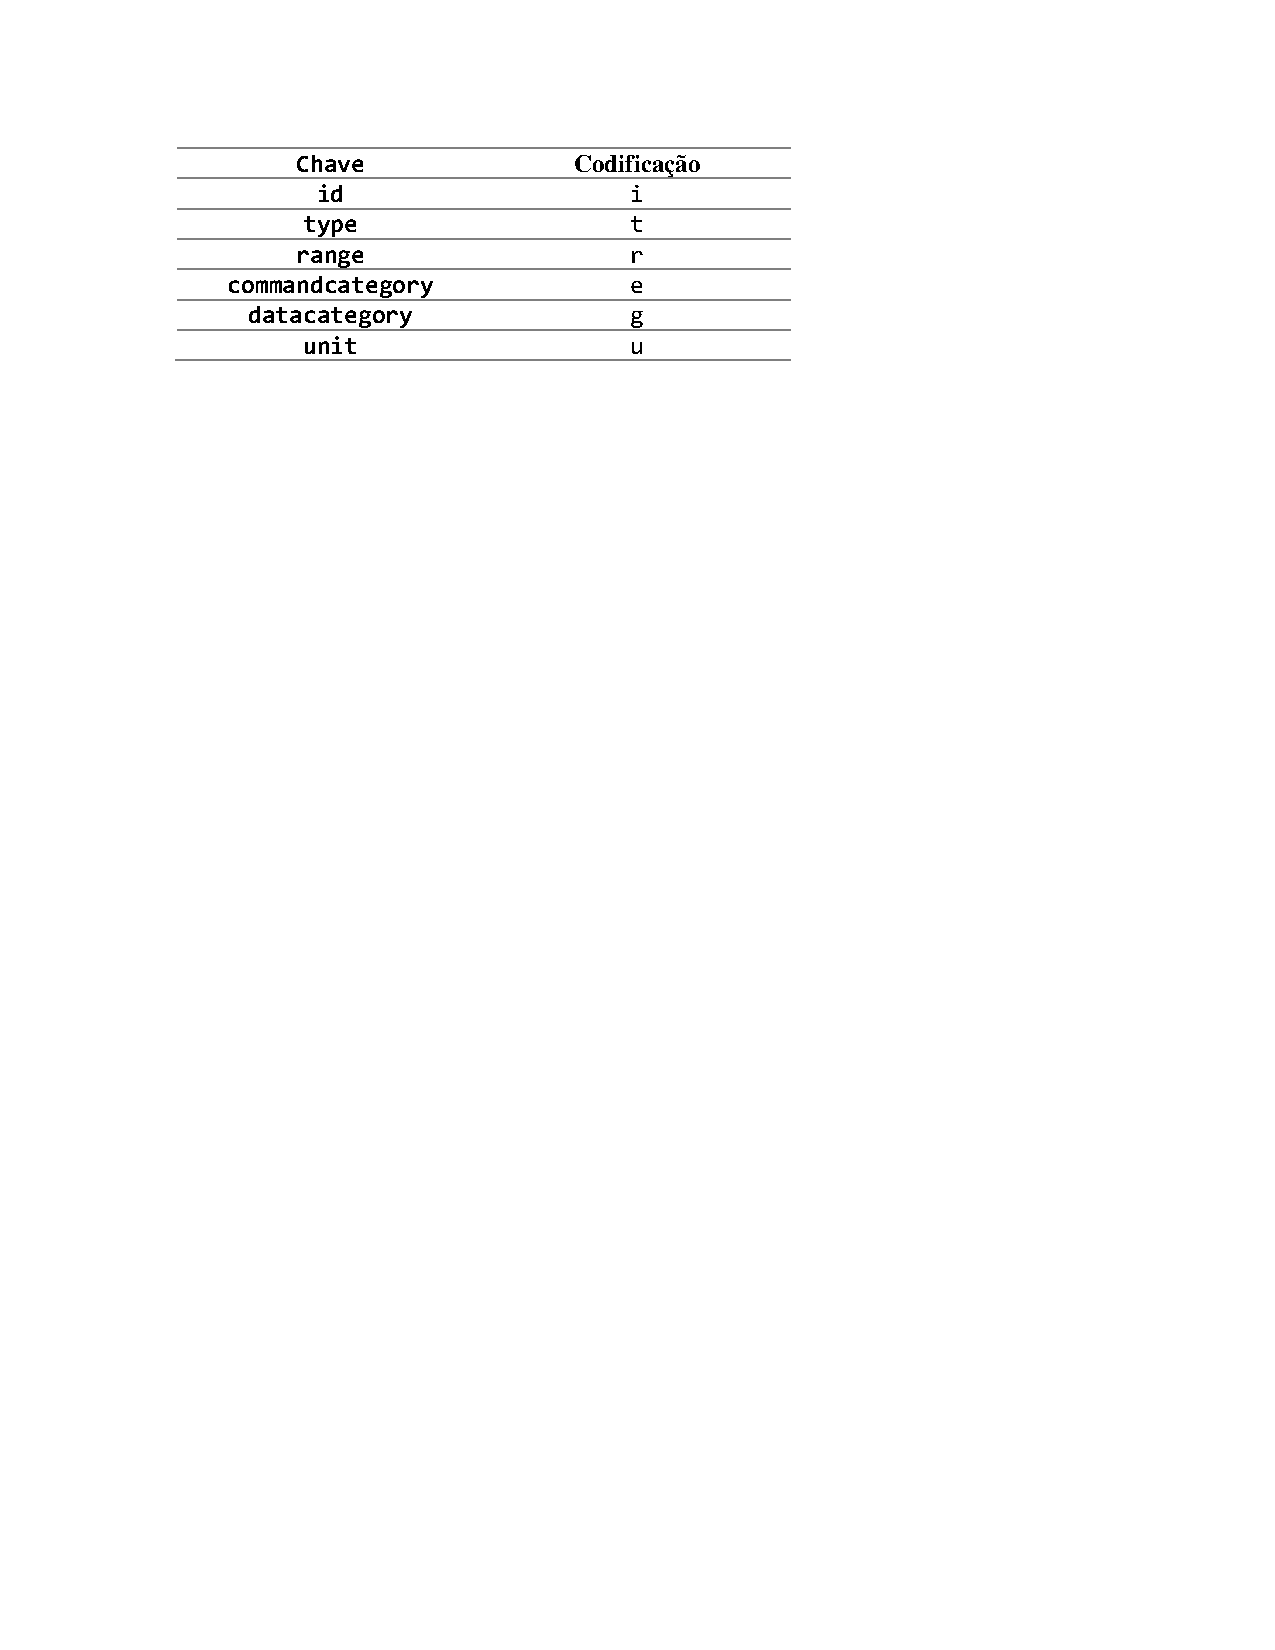
\includegraphics[width=0.7\textwidth]{tabelas/codificacao_tipo_dc.pdf}
	
	\caption{Codifica��o de chaves utilizadas em mensagens do tipo \texttt{data} e \texttt{command}.}\smallskip
	\label{tab:codificacao_dc}
	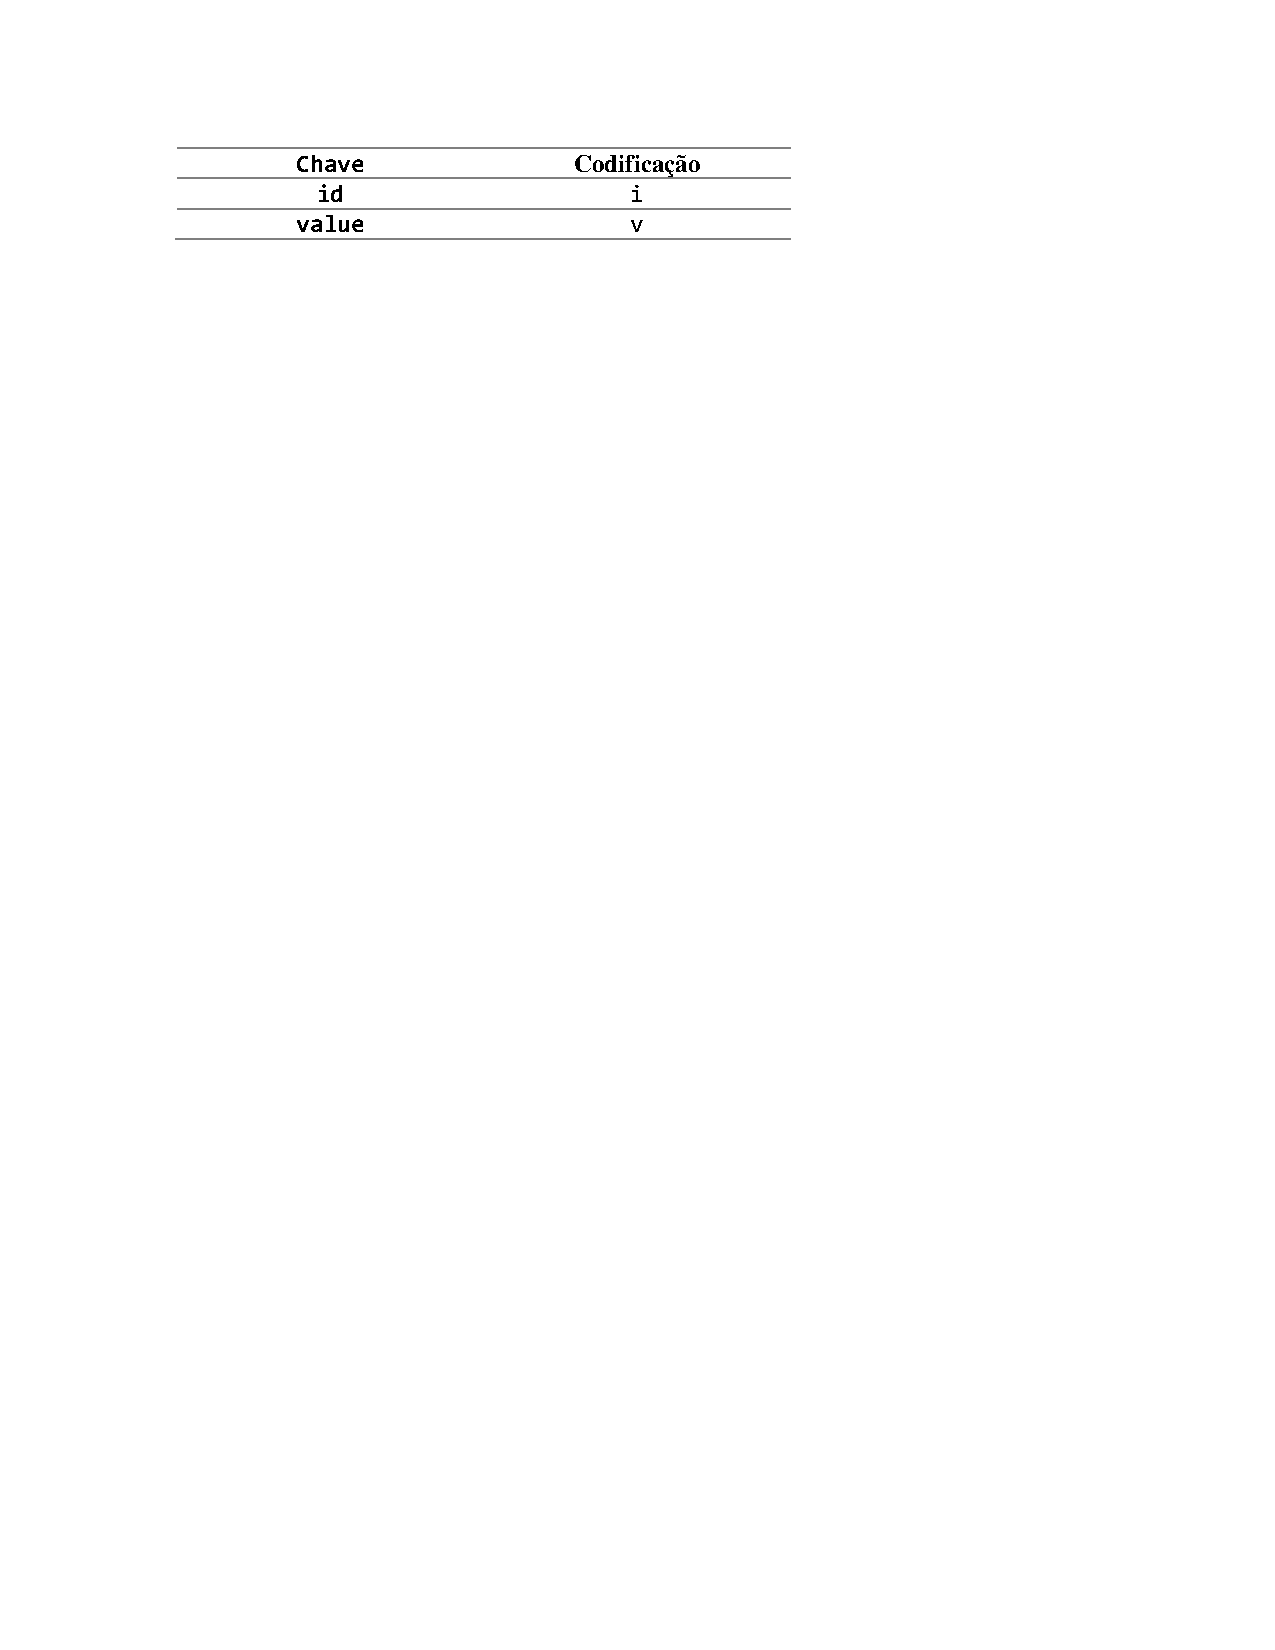
\includegraphics[width=0.7\textwidth]{tabelas/codificacao_dc.pdf}
	
\end{table}

De modo similar, as Tabelas \ref{tab:cod_valores_packagetype}, \ref{tab:cod_valores_nodeclass}, \ref{tab:cod_valores_measurestrat}, \ref{tab:cod_data_category}, \ref{tab:cod_command_category} e \ref{tab:cod_type_category} listam as codifica��es adotadas para os valores utilizados em diversos campos das mensagens. Observe que os valores utilizados nos campos \texttt{packageType} (Tabela \ref{tab:cod_valores_packagetype}) e \texttt{nodeClass} (Tabela \ref{tab:cod_valores_nodeclass}) evoluem em pot�ncias de 2. Isso ocorre pois, conforme apontado na se��o \ref{subsec:sintaxe}, tais campos permitem m�ltiplos valores. Deste modo, a representa��o de mais de um valor � feita efetuando-se uma opera��o de OR bin�rio. Por exemplo, se um dado dispositivo for tanto sensor (c�digo 1) quanto atuador (c�digo 2), sua representa��o se dar� enviando um pacote contendo o campo \texttt{nodeClass} definido para 3.

\begin{table}[hp]
	\centering
	\caption{Codifica��o dos valores do campo \texttt{packageType}.}\smallskip
	\label{tab:cod_valores_packagetype}
	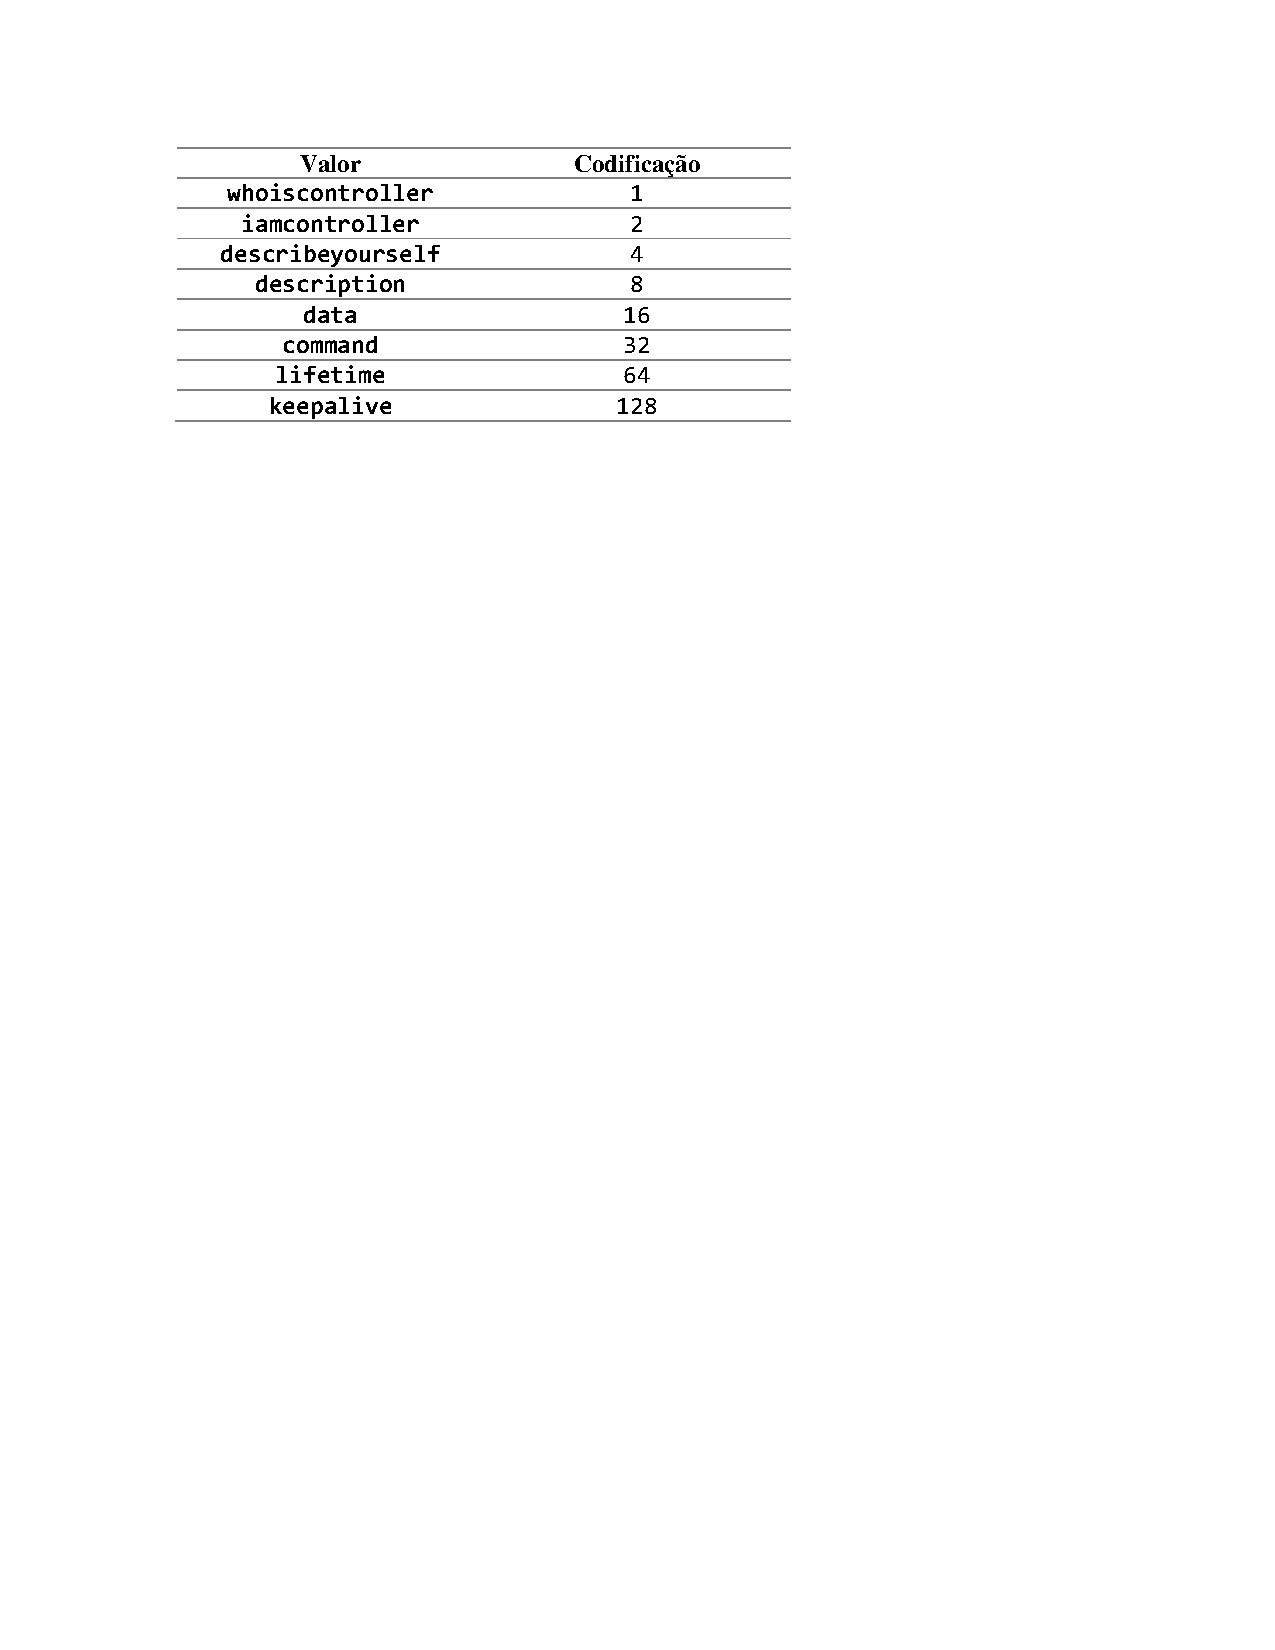
\includegraphics[width=0.7\textwidth]{tabelas/cod_valores_packagetype.pdf}
\end{table}

\begin{table}[hp]	
	\centering
	\caption{Codifica��o de valores do campo \texttt{nodeClass}.}\smallskip
	\label{tab:cod_valores_nodeclass}
	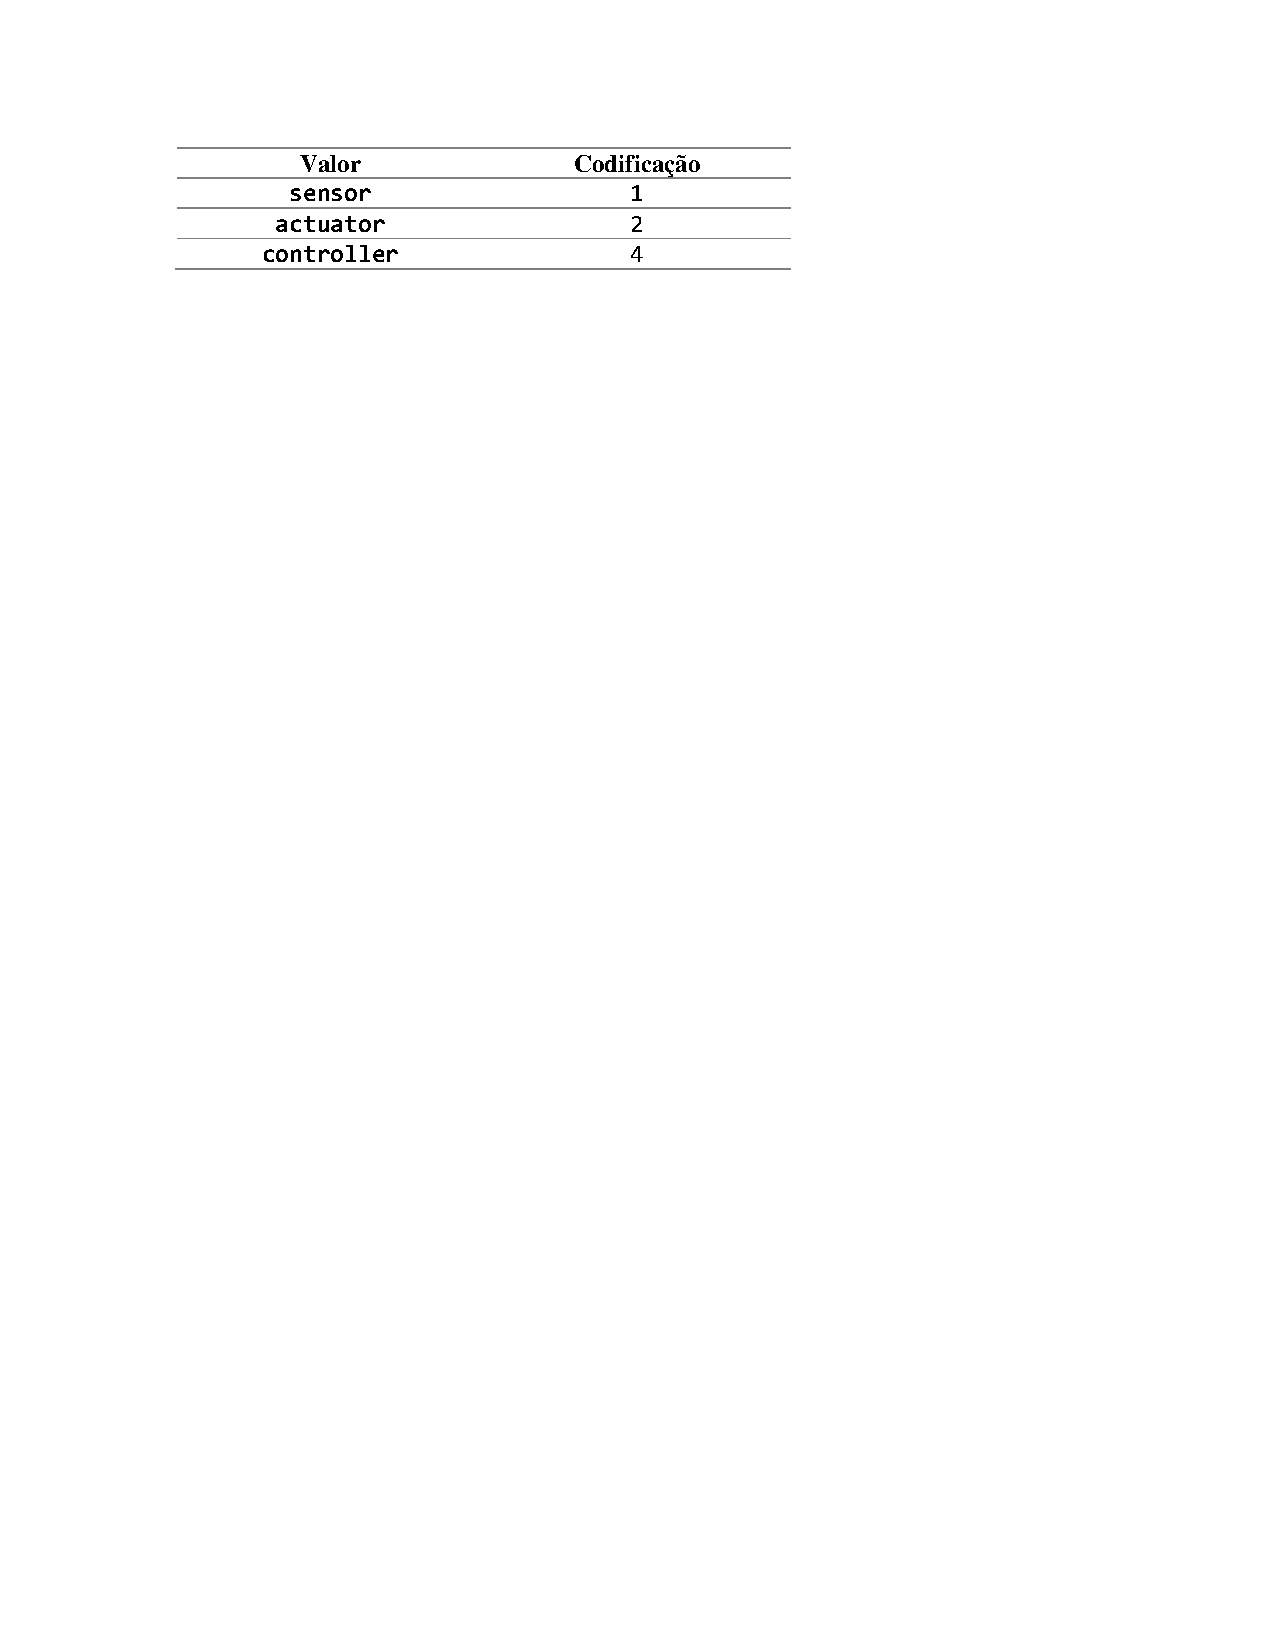
\includegraphics[width=0.7\textwidth]{tabelas/cod_valores_nodeclass.pdf}
\end{table}

\begin{table}[hp]	
	\centering
	\caption{Codifica��o de valores do campo \texttt{measureStrategy}.}\smallskip
	\label{tab:cod_valores_measurestrat}
	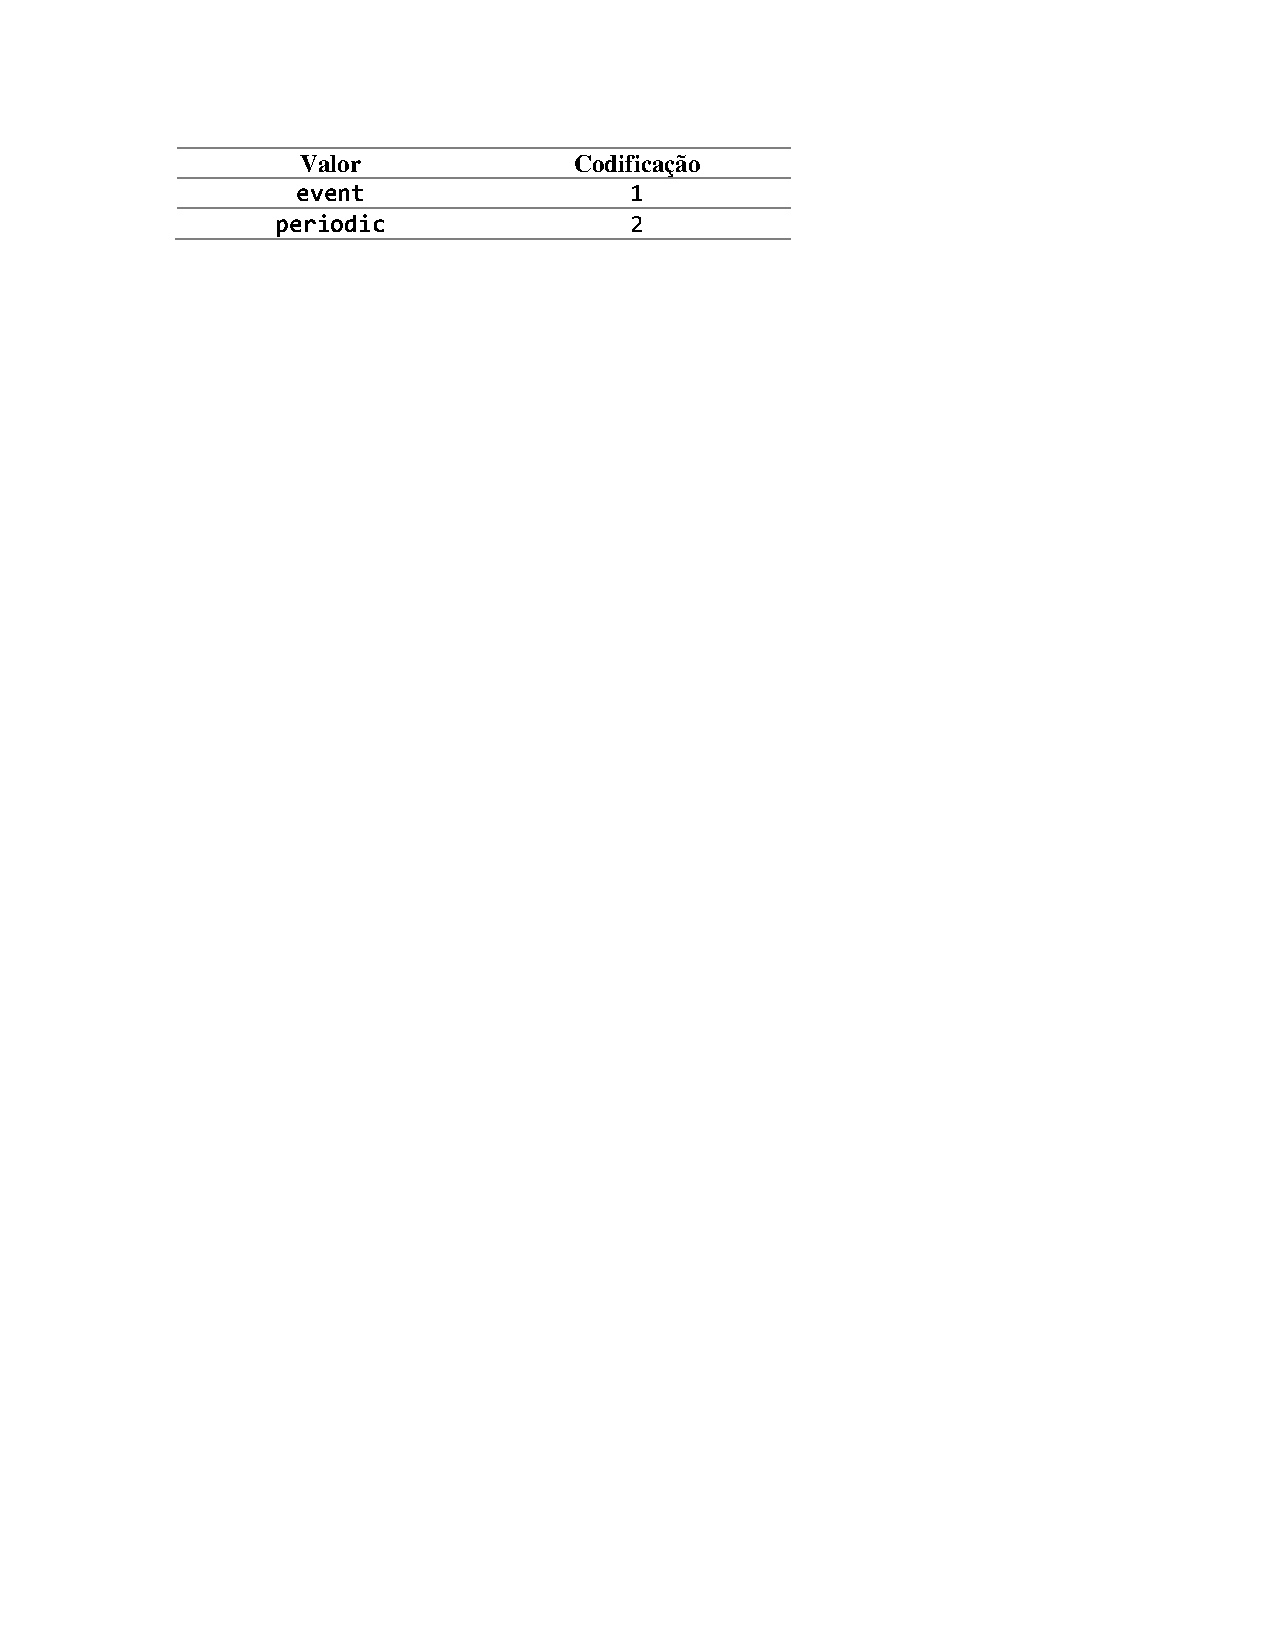
\includegraphics[width=0.7\textwidth]{tabelas/cod_valores_measurestrat.pdf}
\end{table}

\begin{table}[hp]	
	\centering
	\caption{Codifica��o de valores de categoria para sensores}\smallskip
	\label{tab:cod_data_category}
	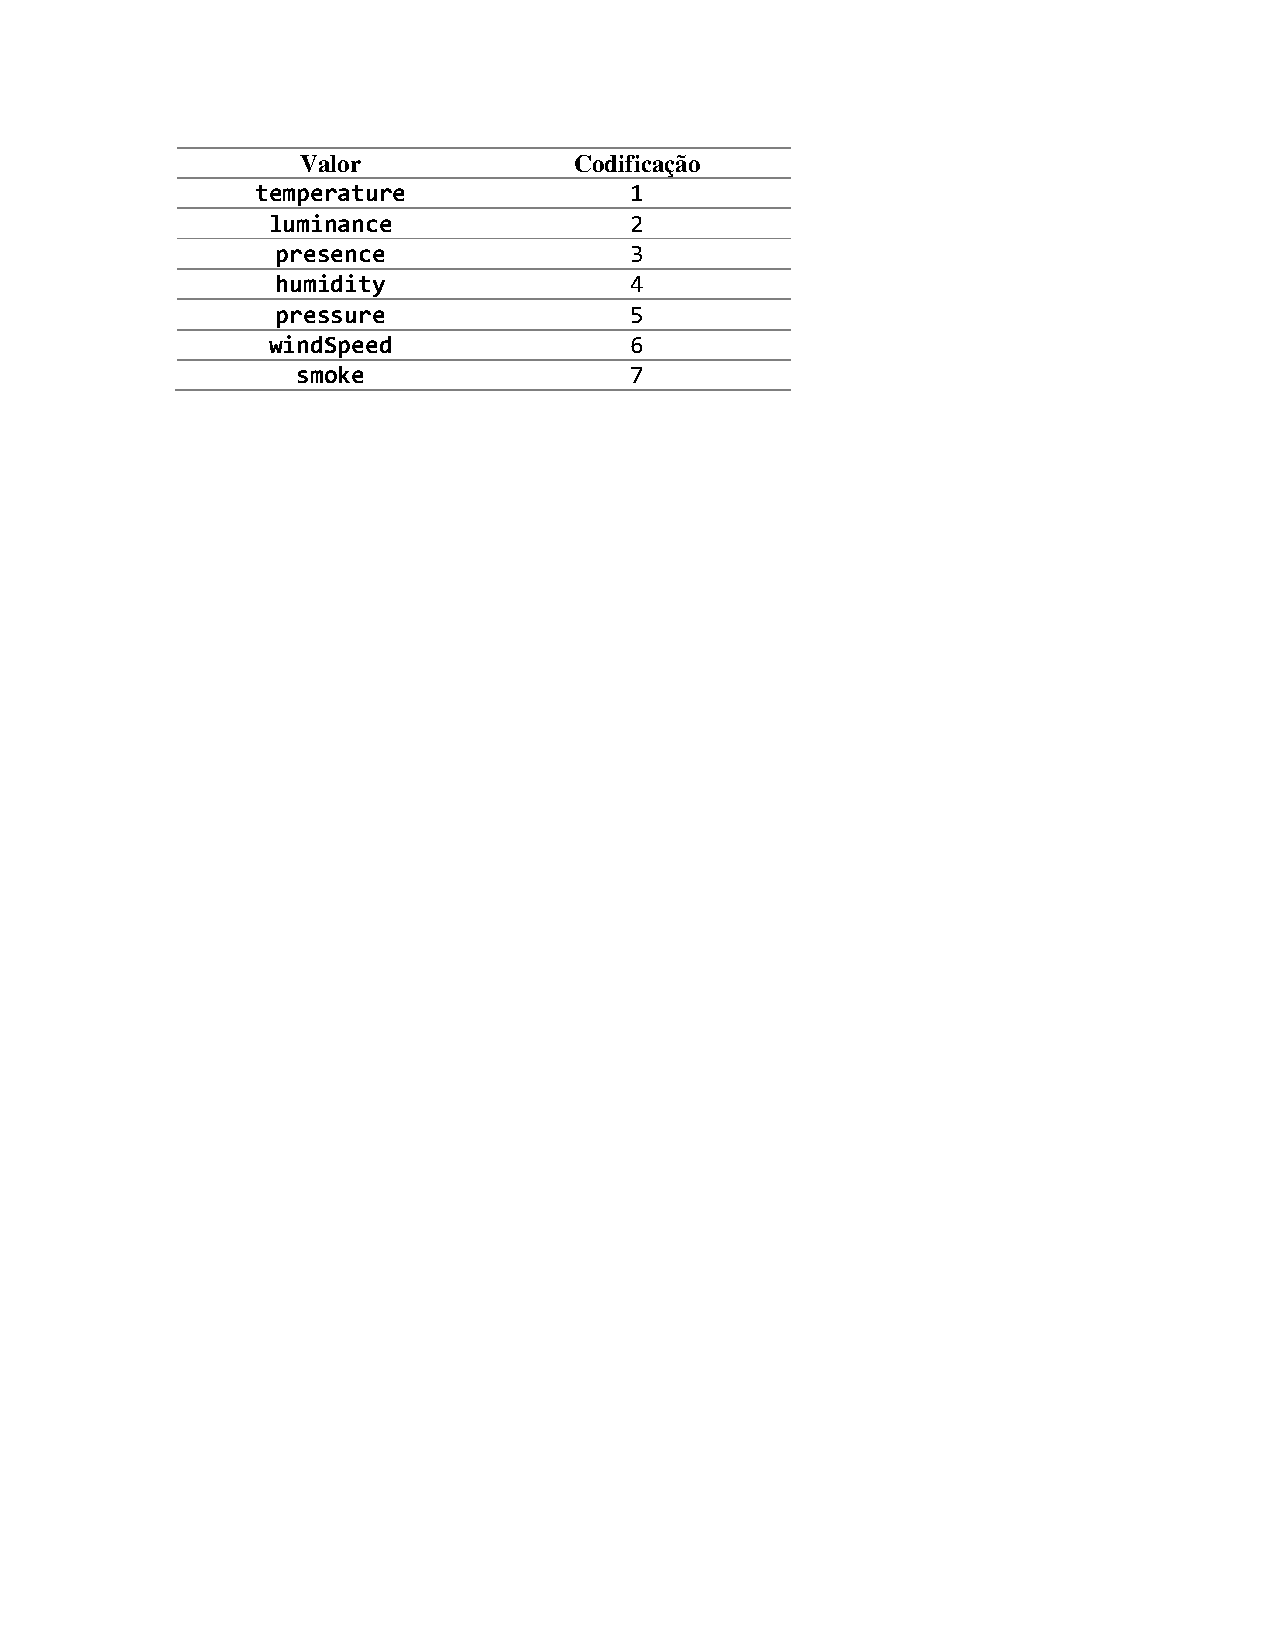
\includegraphics[width=0.7\textwidth]{tabelas/cod_data_category.pdf}
\end{table}

\begin{table}[hp]	
	\centering
	\caption{Codifica��o de valores de categoria para atuadores}\smallskip
	\label{tab:cod_command_category}
	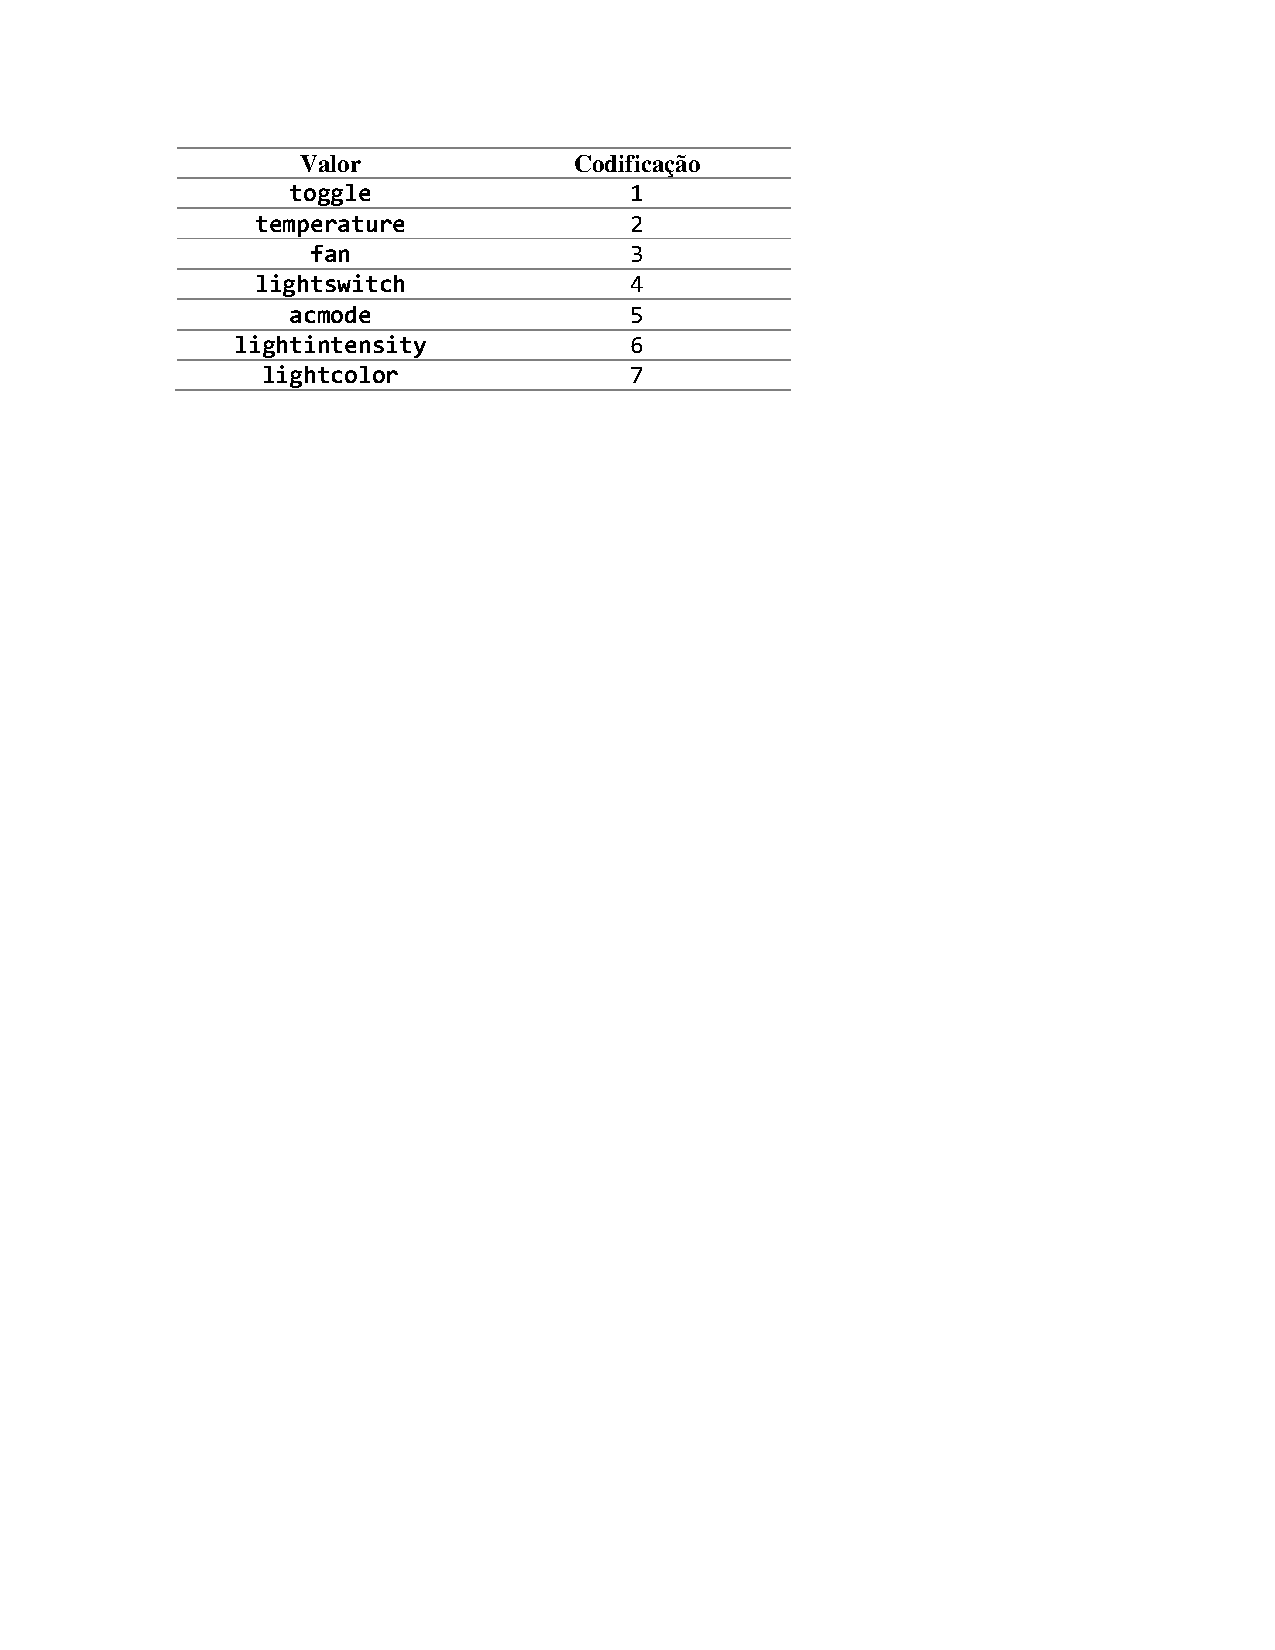
\includegraphics[width=0.7\textwidth]{tabelas/cod_command_category.pdf}
\end{table}

\begin{table}[hp]	
	\centering
	\caption{Codifica��o de tipos de dados e comandos}\smallskip
	\label{tab:cod_type_category}
	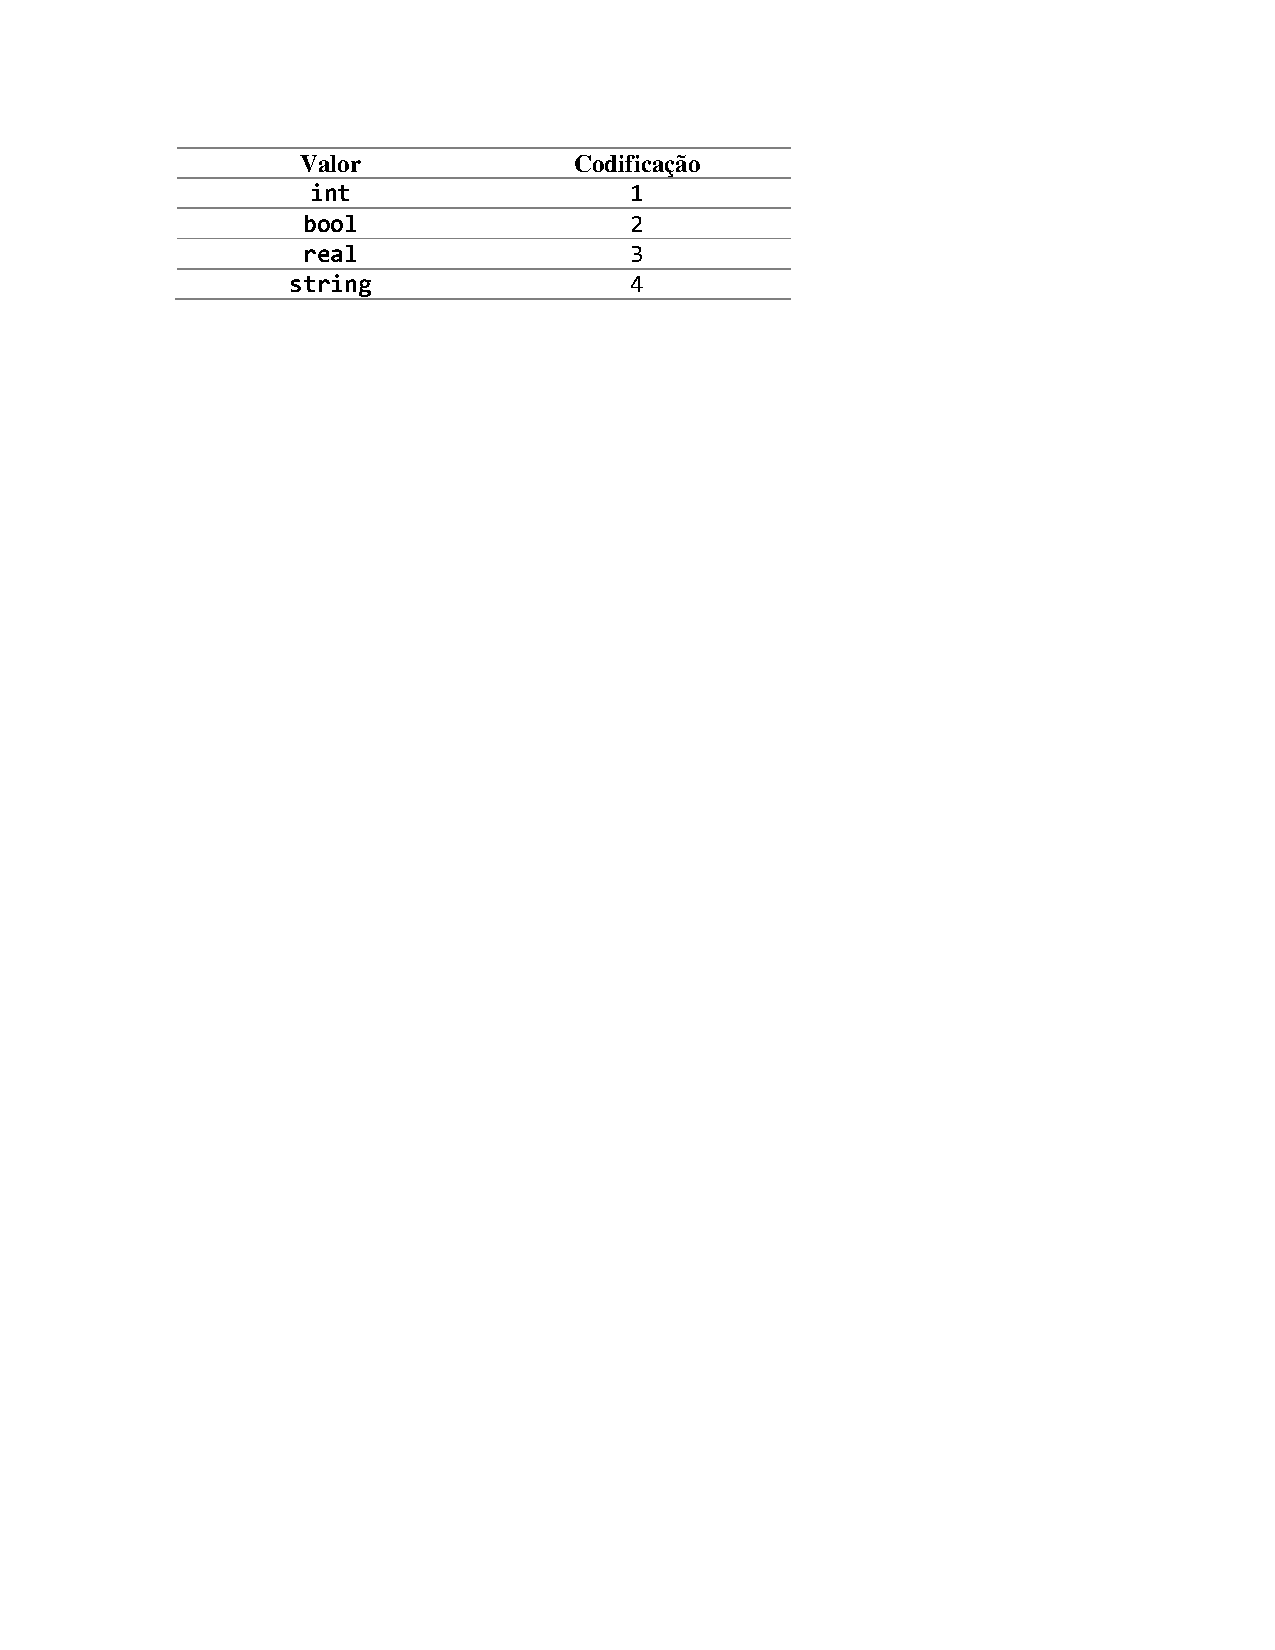
\includegraphics[width=0.7\textwidth]{tabelas/cod_type_category.pdf}
\end{table}

\clearpage
A Figura \ref{fig:tamanho_pacote} mostra os resultados da aplica��o das t�cnicas de compress�o de tamanho aos pacotes enviados. No gr�fico, s�o comparados os tamanhos de cada tipo de pacote em tr�s codifica��es: JSON original (todos os campos s�o \textit{strings} leg�veis, JSON com campos e valores mapeados conforme documentado nesta se��o, e JSON mapeado seguido da aplica��o da codifica��o CBOR.

\begin{figure}[h]
	\centering
	\caption{Tamanho resultante do pacote em fun��o da codifica��o aplicada}
	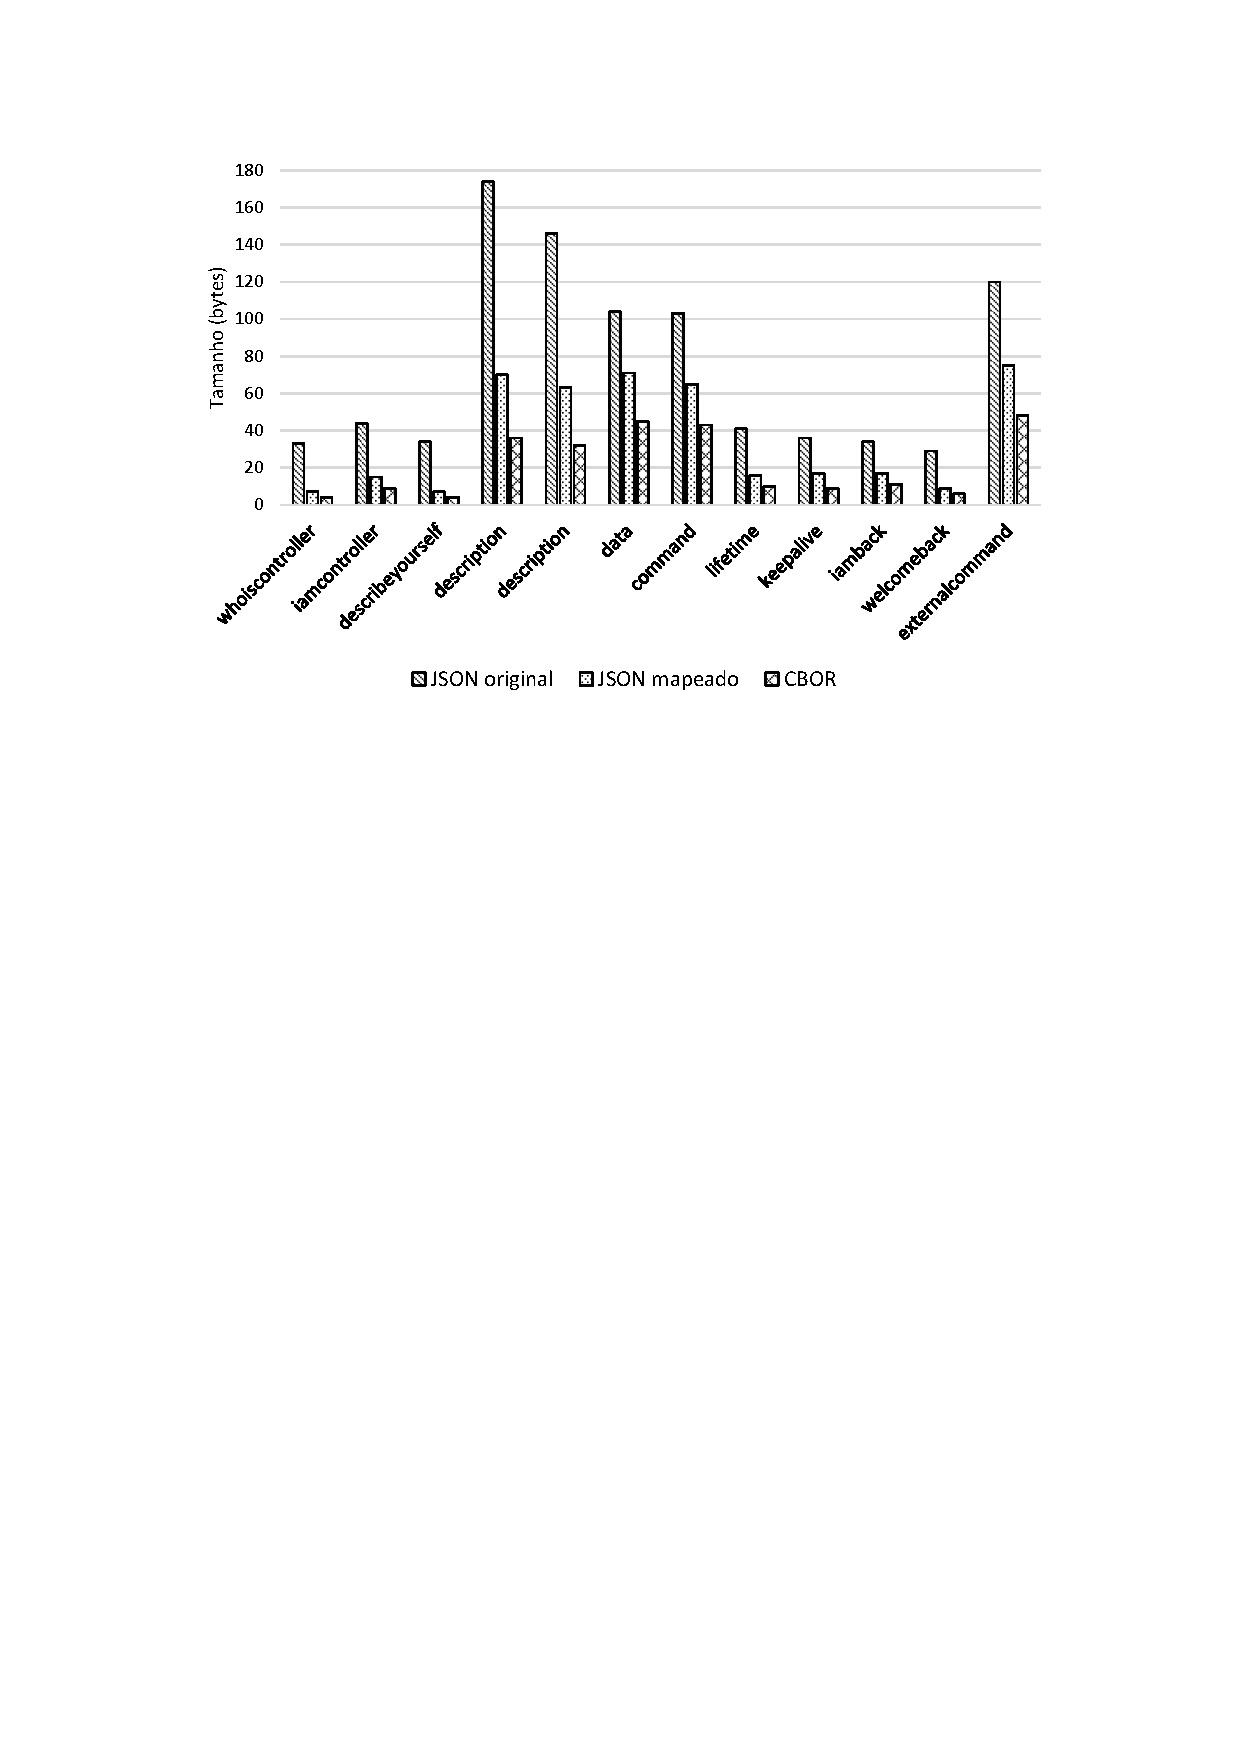
\includegraphics[width=\textwidth]{imagens/tamanho_pacote.pdf}
 	\label{fig:tamanho_pacote}
\end{figure}

Do gr�fico, verifica-se que houve redu��o m�dia de aproximadamente 74\% no tamanho dos pacotes, representando uma redu��o significativa na quantidade de dados transmitidos na rede. No entanto, em termos pr�ticos, espera-se que pacotes do tipo \texttt{data} e \texttt{command} sejam os mais frequentes em uma rede, visto que os demais ocorrem principalmente durante o \textit{handshake} inicial. A redu��o de tamanho verificada nestes pacotes foi de 56\% e 58\%, respectivamente, logo espera-se que haja uma redu��o efetiva no tamanho dos pacotes pr�xima a esses valores. 

\subsection{Exemplo de Funcionamento}
Para ilustrar o funcionamento do protocolo, considere a rede mostrada na Figura \ref{fig:exemplo_rede}. Nesta rede, existem um sensor (bot�o), um atuador (interruptor de luz) e um controlador local interligando-os. O bot�o funciona como um sensor com estado bin�rio: a cada acionamento, seu estado � invertido. De modo similar, o interruptor aceita comandos em formato bin�rio, fechando o contato caso um comando "1" seja recebido e abrindo caso "0" seja recebido.

\begin{figure}[h]
	\centering
	\caption{Exemplo de aplica��o do protocolo \textit{Rainfall}.}
	
\includegraphics[width=0.7\textwidth]{imagens/exemplo_rede.png}
 	\label{fig:exemplo_rede}
\end{figure}

A Figura \ref{fig:exemplo_handshake} ilustra o processo de \textit{handshake} no exemplo dado. Observe que as mensagens j� exploram a possibilidade de enviar m�ltiplas mensagens em um mesmo pacote, tal como mostrado na Figura \ref{fig:uml_handshake}.

\begin{figure}[hp]
	\centering
	\caption{Processo de \textit{handshake} no exemplo.}
	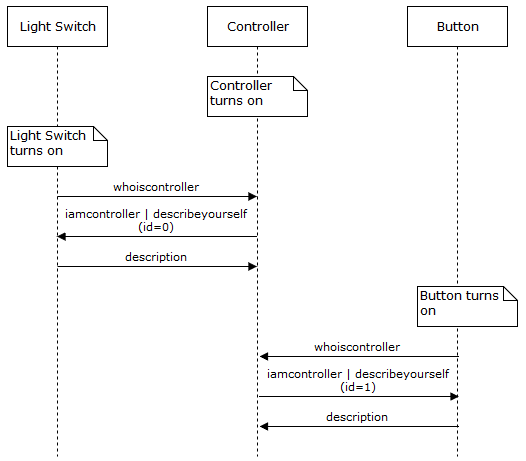
\includegraphics[width=0.9\textwidth]{imagens/exemplo_handshake.png}
 	\label{fig:exemplo_handshake}
\end{figure}

A Figura \ref{fig:exemplo_dados} ilustra o processo de troca de dados e o envio de comandos na rede de exemplo. No caso, o controlador foi configurado com as seguintes regras:
\begin{itemize}
	\item Caso o bot�o envie um dado "0", o comando "0" (abrir contato ou apagar a luz) � enviado ao interruptor;
	\item Caso o bot�o envie um dado "1", o comando "1" (fechar contato ou acender a luz) � enviado ao interruptor.
\end{itemize}

\begin{figure}[hp]
	\centering
	\caption{Processo de troca de dados e aplica��o de regras no exemplo.}
	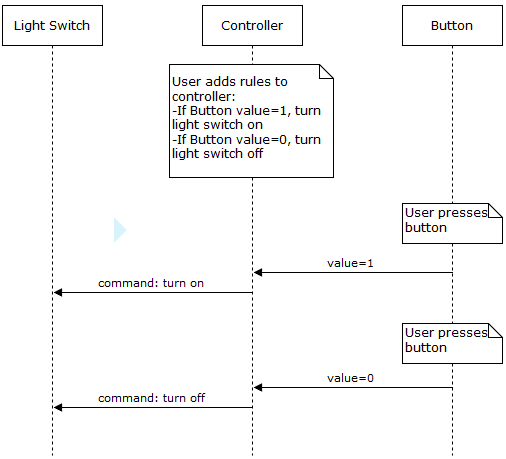
\includegraphics[width=0.9\textwidth]{imagens/exemplo_dados.png}
 	\label{fig:exemplo_dados}
\end{figure}

\clearpage

\section{Implementa��o de Bibliotecas para o Protocolo de Aplica��o} \label{sec:implsens}
Uma vez analisados os protocolos de comunica��o existentes e definido o protocolo de aplica��o, passa-se para o projeto de uma biblioteca que permita o desenvolvimento de dispositivos em conformidade com ele.

\subsection{Arquitetura}
A biblioteca desenvolvida possuir� uma arquitetura em camadas, conforme ilustra a Figura \ref{fig:libarchitecture}. As camadas apresentadas em cor verde comp�em a biblioteca a ser desenvolvida no projeto. A descri��o de cada camada est� apresentada a seguir.

\begin{figure}[h]
	\centering
	\caption{Arquitetura em camadas da biblioteca}
	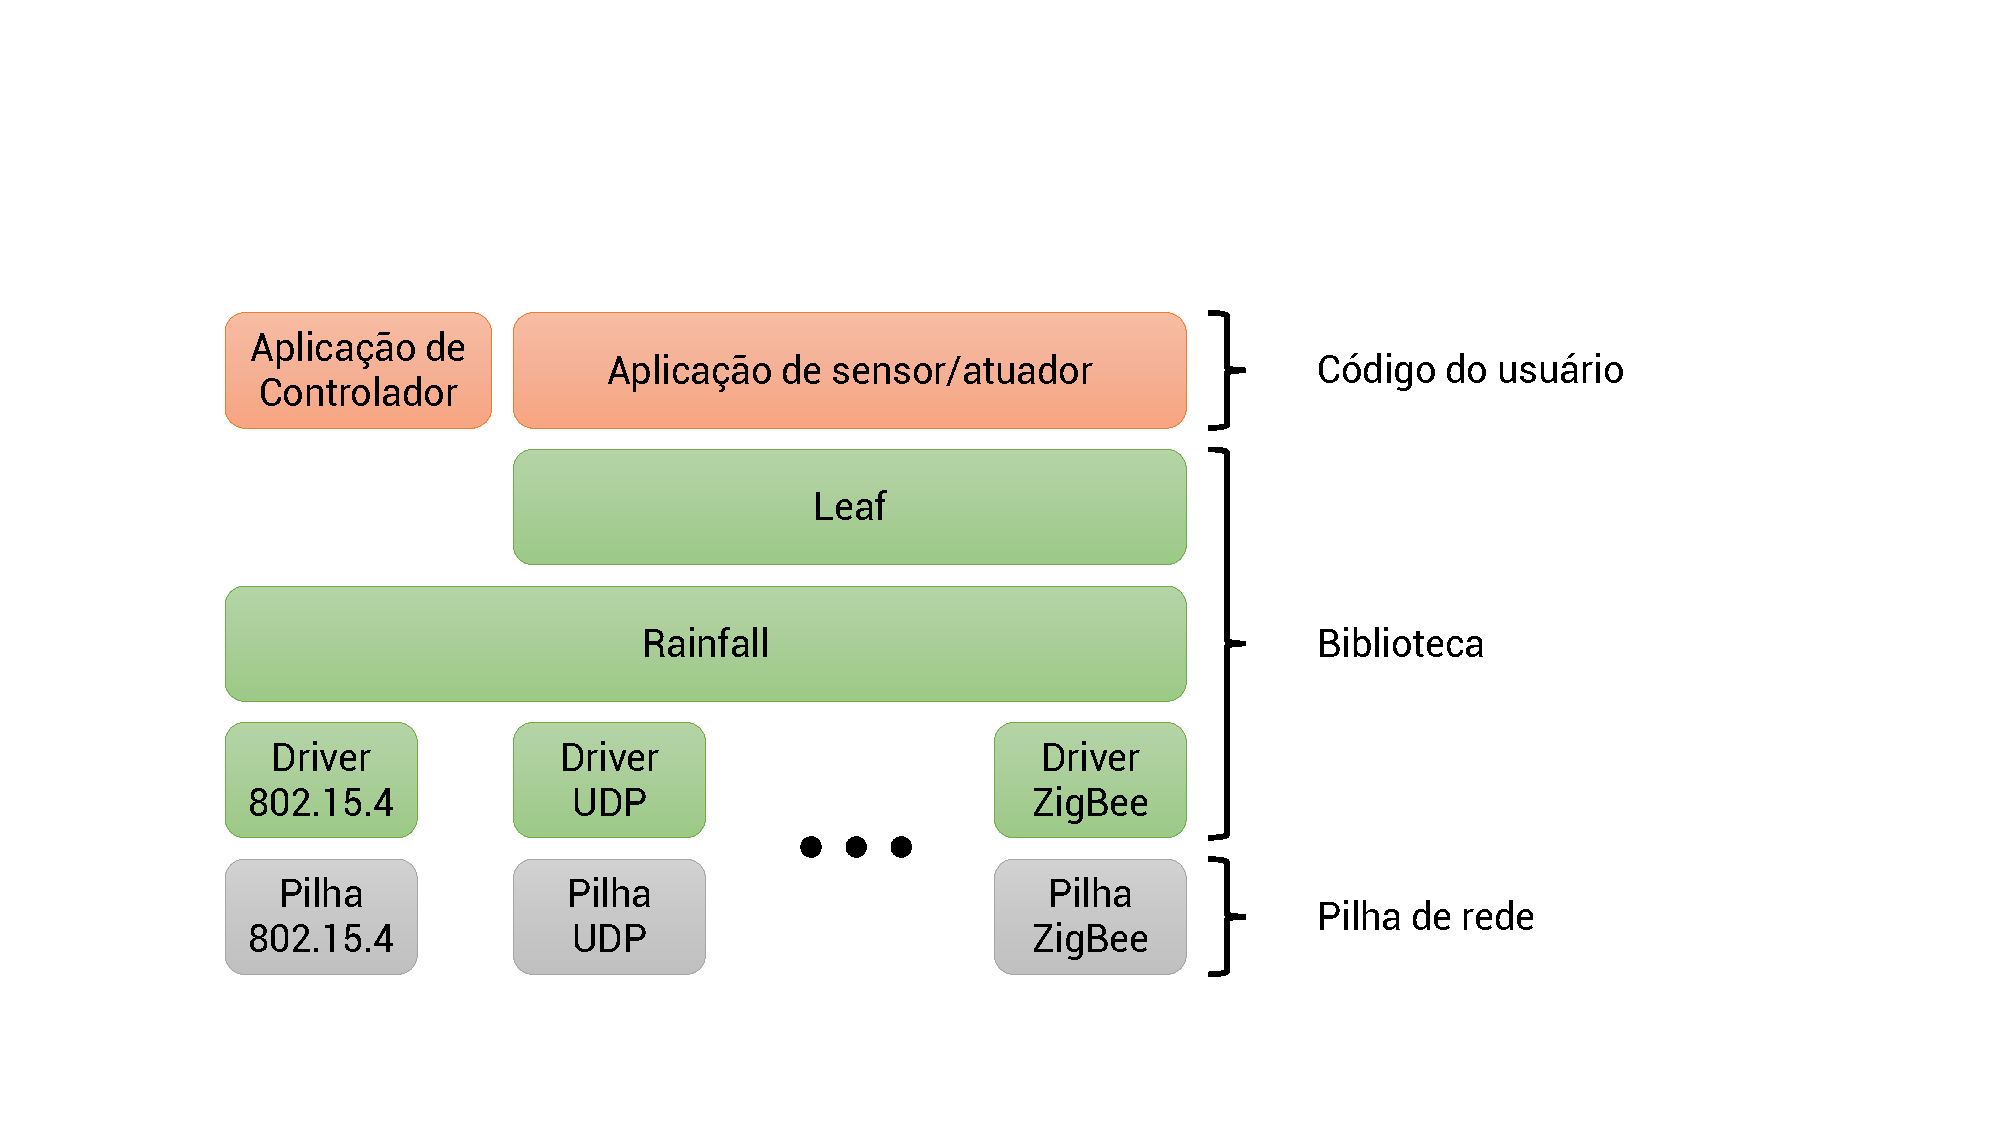
\includegraphics[width=0.8\textwidth]{imagens/libarchitecture.pdf}
 	\label{fig:libarchitecture}
\end{figure}

\paragraph*{Drivers de rede.} A primeira camada da biblioteca consiste em drivers de rede, que proveem uma interface com as diferentes pilhas de rede existentes (cf. item \ref{sec:commprot}). Esta � a �nica camada da biblioteca que possui depend�ncias com as particularidades de cada protocolo ou dispositivo de rede. Possui a fun��o de prover um acesso uniformizado para fun��es comuns utilizadas pelas camadas superiores, tais como escutar e enviar pacotes.

\paragraph*{Biblioteca \textit{Rainfall}.} Esta camada tem como objetivo efetuar a transforma��o de um objeto estruturado segundo as especifica��es do protocolo \textit{Rainfall} e codific�-lo no formato de envio (mapeando campos e valores para n�meros, e codificando no formato CBOR), e vice-versa. Al�m disso, ele efetua checagens sint�ticas dos pacotes enviados, verificando se somente campos permitidos s�o utilizados para cada tipo de pacote, conforme as regras apresentadas no item \ref{subsec:sintaxe}. Observe que esta camada atua como um \textit{middleware}, provendo uma interface comum entre a l�gica de aplica��o e os diversos protocolos de rede.

\paragraph*{Biblioteca \textit{Leaf}.} Esta camada atua sobre as fun��es fornecidas pela \textit{Rainfall}, fornecendo uma API que abstrai os detalhes do protocolo. Por exemplo, o processo de inicializa��o mostrado na Figura \ref{fig:uml_handshake} � abstra�do atrav�s de um m�todo de inicializa��o disponibilizado nesta biblioteca.

\paragraph*{Aplica��es de usu�rio.} As bibliotecas desenvolvidas permitem o desenvolvimento de \textit{software} de controle de dispositivos em conformidade com as especifica��es do protocolo \textit{Rainfall}. Dispositivos sensores e atuadores podem ser desenvolvidos facilmente atrav�s da biblioteca \textit{Leaf}, ao passo que a l�gica de um dispositivo controlador pode ser descrita utilizando-se a biblioteca \textit{Rainfall} diretamente.

\subsection{Implementa��o e Exemplos}
Uma implementa��o das bibliotecas para desenvolvimento de dispositivos seguindo o protocolo \textit{Rainfall} foi feita utilizando a linguagem JavaScript, utilizando o ambiente Node.js\footnote{Dispon�vel em \url{https://nodejs.org/}.}. O c�digo-fonte desta implementa��o, al�m de exemplos de uso da biblioteca para o desenvolvimento de sensores, atuadores e controladores, est�o hospedados no servi�o GitHub \footnote{Dispon�vel no endere�o \url{https://github.com/HomeSkyLtd/}}.

\section{Limita��es e N�o-escopos}
O projeto do protocolo de comunica��o foi feito com o objetivo de prover um meio de troca de informa��es entre dispositivos e controladores de uma rede de sensores. Entretanto, dado o contexto de um projeto de conclus�o de curso, alguns aspectos n�o foram enfatizados no presente momento, a despeito de sua import�ncia em aplica��es reais. O grupo adotou algumas hip�teses simplificadoras, listadas nas se��es a seguir.

\subsection{Conectividade}
As seguintes hip�teses foram feitas no quesito de conectividade dos dispositivos:
\begin{itemize}
	\item N�s se encontram conectados � rede. No projeto do protocolo e na implementa��o das bibliotecas, n�o se tratou o processo de conex�o dos dispositivos � rede em que o controlador opera. Ou seja, foi considerado que o usu�rio � capaz de conectar os dispositivos � rede desejada. Existem tecnologias que permitem efetuar conex�o de um dispositivo � rede sem necessidade de interface gr�fica ou inser��o de senhas, tal como o Wi-Fi Protected Setup (WPS), que podem ser utilizados para este fim;
	\item Protocolos de comunica��o e/ou transporte subjacentes s�o confi�veis. No projeto do protocolo, n�o se tratou o reconhecimento de entrega das mensagens, pois sup�s-se que os protocolos de rede ou transporte subjacentes ao de aplica��o garantem entrega dos pacotes ao destinat�rio. Essa � uma estimativa razo�vel, visto que os protocolos de rede para redes de sensores sem fio assumem que as condi��es de transmiss�o s�o adversas, e incluem mecanismos de retransmiss�o. No entanto, caco se deseje utilizar um protocolo n�o confi�vel, como o UDP, seria poss�vel adicionar um mecanismo de envio de ACKs em n�vel de aplica��o para garantir a entrega.
\end{itemize}

\subsection{Seguran�a}
As seguintes hip�teses foram feitas no quesito de seguran�a do sistema:
\begin{itemize}
	\item A infraestrutura de rede � segura. O grupo assumiu que a rede onde os dispositivos atuar�o � configurada de forma segura, utilizando algoritmos criptogr�ficos e senhas adequadas. Deste modo, usu�rios n�o autorizados ou mal-intencionados n�o seriam capazes de conectar dispositivos � rede de sensores dom�stica. Um modo de tratar o caso em que redes inseguras s�o utilizadas seria enviar notifica��es ao usu�rio a cada n� novo conectado, perguntando se a conex�o ao controlador deve ser permitida;
	\item N�s da rede atuam conforme esperado. Sup�e-se que n�s de rede sejam configurados para operar em conformidade com o protocolo. Por exemplo, um sensor n�o responderia a mensagens destinadas a outros dispositivos, ou n�o fingiria ser o controlador. Uma maneira de se assegurar tal comportamento "honesto" seria atrav�s da efetua��o de homologa��o de dispositivos.
\end{itemize}
\chapter{Projeto do Servi�o em Nuvem}\label{chp:serviconuvem}
Este cap�tulo possui a finalidade de projetar e implementar um servi�o em nuvem acess�vel aos controladores locais da rede de sensores, de modo a alcan�ar o objetivo (ii) do trabalho. Os t�picos abordados neste cap�tulo englobam o protocolo de troca de dados envolvendo o servidor em nuvem (batizado de Homecloud), a interface de controle do usu�rio e a especifica��o de um algoritmo de aprendizagem espec�fico para o dom�nio de controle de ilumina��o.

\section{O Protocolo Homecloud}
Conforme mencionado na se��o \ref{sec:arquitetura}, o servidor em nuvem se comunica tanto com o controlador local quanto com o dispositivo de interface do usu�rio. O protocolo Homecloud, definido pelo grupo, define o formato das mensagens a serem trocados pelos dispositivos, e em quais circunst�ncias. As pr�ximas se��es especificar�o em detalhes o funcionamento deste protocolo.

\subsection{Sintaxe e Sem�ntica}
Para melhor organizar as mensagens do protocolo, elas ser�o agrupadas no decorrer deste relat�rio em quatro classes de acordo com a sua fun��o, a saber:

\begin{itemize}
	\item Mensagens de Estado: Transmitem informa��es relativas ao estado da casa, incluindo dados lidos de sensores, estados de atuadores e a��es tomadas pelo usu�rio;
	\item Mensagens de Regras: Referem-se � defini��o de regras de automa��o pelo usu�rio ou pelo sistema de aprendizagem de m�quina;
	\item Mensagens de Gerenciamento dos N�s: Transmitem informa��es e comandos relativos aos n�s (sensores e atuadores) da rede local;
	\item Mensagens de Autentica��o: Respons�veis por carregar dados de autentica��o dos agentes do sistema.
\end{itemize}

As mensagens s�o enviadas ao servidor atrav�s de requisi��es HTTP. Portanto, cada mensagem uma resposta de um determinado tipo, a depender da natureza das informa��es solicitadas.  Notifica��es destinadas aos usu�rios ou aos controladores n�o esperam resposta, pois s�o enviadas por meio protocolos que n�o esperam resposta. 

A seguir ser�o definidas as mensagens, de acordo com a classifica��o apresentada, bem como as respectivas respostas esperadas. 

\subsubsection{Mensagens de Estado}
As mensagens de estado est�o listadas e descritas na Tabela \ref{tab:mensagens_estado}. Nesta tabela, o sentido de tr�fego das mensagens est�o especificadas. Neste item, o termo "aplicativo" foi utilizado para se referir ao dispositivo utilizado pelo usu�rio para interagir com o sistema, que poderia ser um aplicativo em um \textit{smartphone}.

\begin{table}[h]
	\centering
	\caption{Listagem e descri��o das Mensagens de Estado.}\smallskip
	\label{tab:mensagens_estado}
	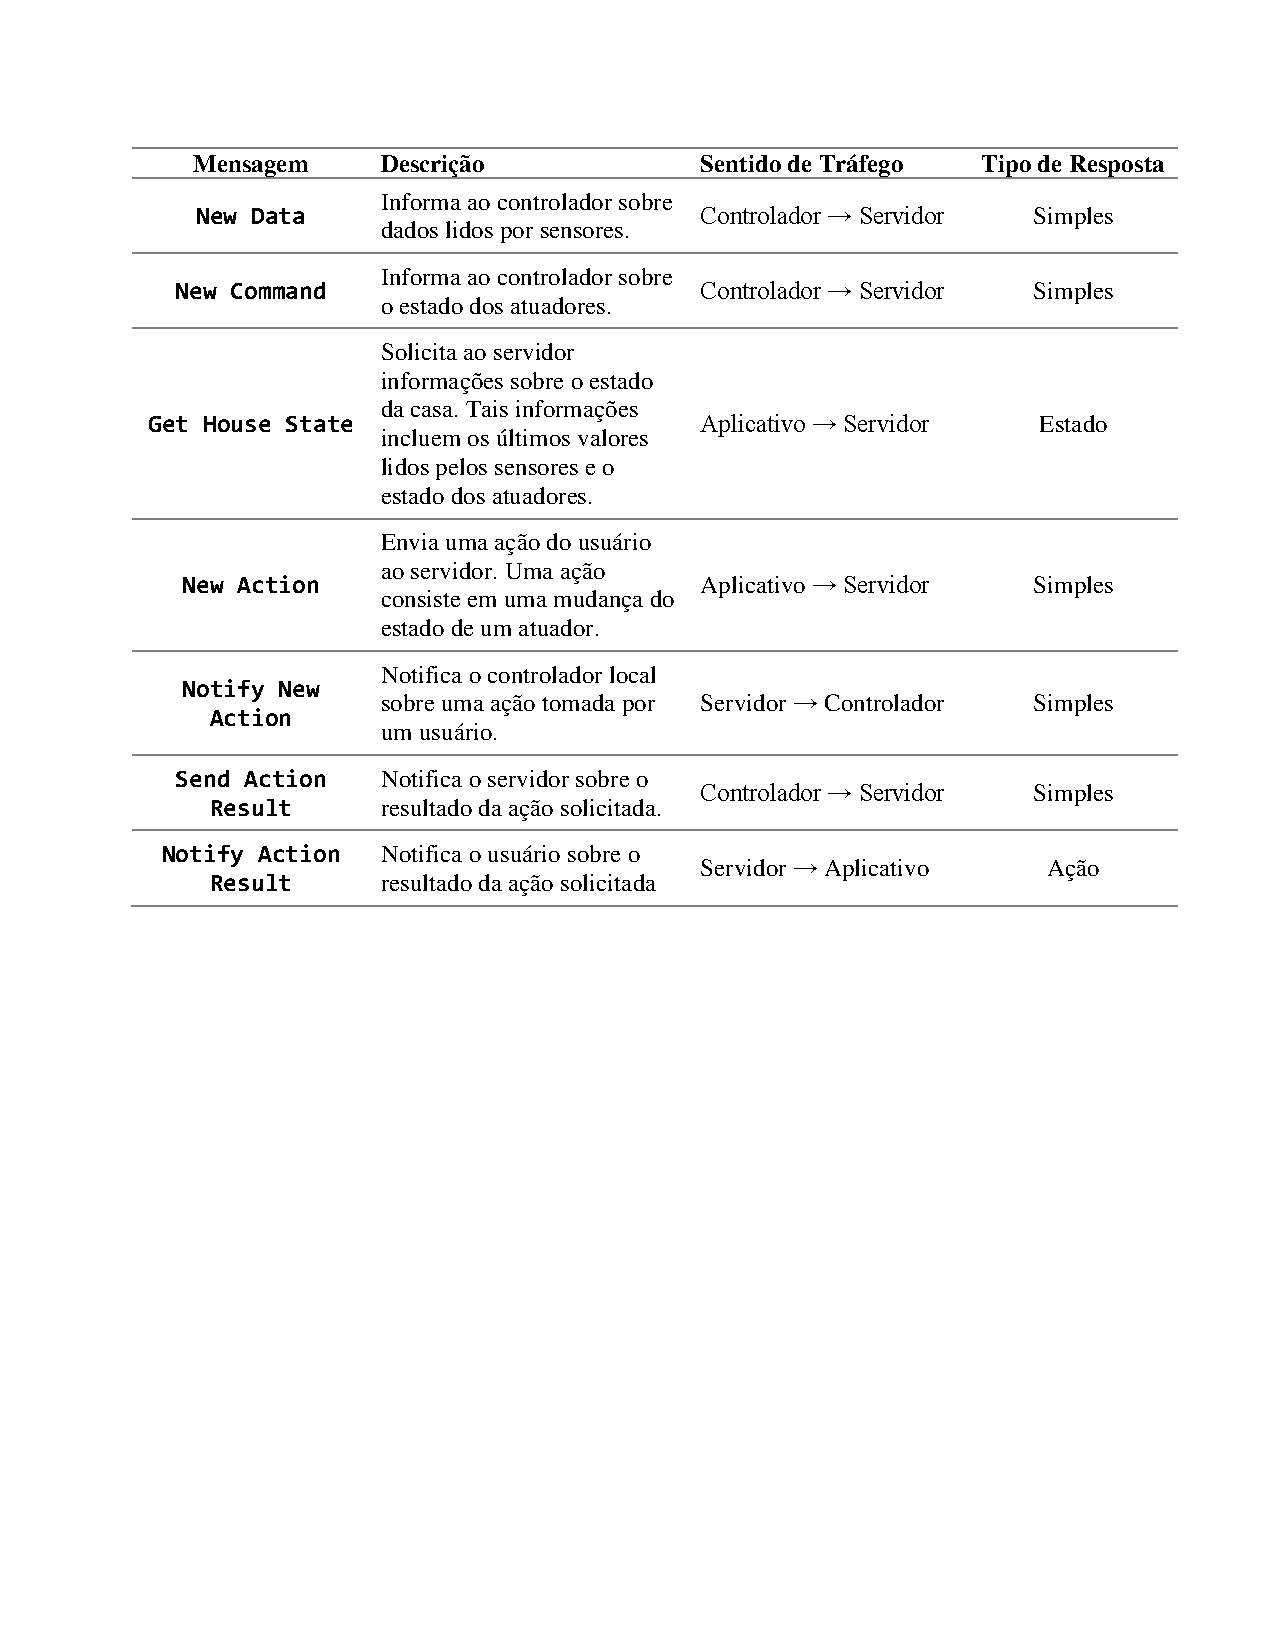
\includegraphics[width=\textwidth]{tabelas/mensagens_estado.pdf}
\end{table}

A seguir, ser� detalhado o conte�do de cada mensagem listada na Tabela \ref{tab:mensagens_estado}. As mensagens seguem o formato JSON, e os campos com valor vari�vel est�o circundados pelos s�mbolos \texttt{< >}.

\paragraph*{\texttt{New Data}.} A Listagem \ref{lst:newData} ilustra o formato da mensagem. O campo \texttt{function} cont�m o nome da mensagem, a ser utilizado pelo servidor para efetuar o tratamento adequado. O campo \texttt{data} cont�m uma lista de objetos, cada qual representando uma leitura de um sensor.

\lstinputlisting[label=lst:newData, caption=Formato da mensagem \texttt{newData}]{codigos/newData.json}

\paragraph*{\texttt{New Command}.} A Listagem \ref{lst:newCommand} ilustra o formato da mensagem. O campo \texttt{command} cont�m uma lista de objetos, cada qual representando uma estado de um atuador.

\lstinputlisting[label=lst:newCommand, caption=Formato da mensagem \texttt{newCommand}]{codigos/newCommand.json}

\paragraph*{\texttt{Get House State}.} A Listagem \ref{lst:getHouseState} ilustra o formato da mensagem.

\lstinputlisting[label=lst:getHouseState, caption=Formato da mensagem \texttt{getHouseState}]{codigos/getHouseState.json}

\paragraph*{\texttt{New Action}.} A Listagem \ref{lst:newAction} ilustra o formato da mensagem. O campo \texttt{action} cont�m um objeto que representa uma a��o a ser tomada. Lembre-se de que uma a��o � definida pelo estado de um comando de um atuador, que o usu�rio supostamente deseja alterar.

\lstinputlisting[label=lst:newAction, caption=Formato da mensagem \texttt{newAction}]{codigos/newAction.json}

\paragraph*{\texttt{Notify New Action}.} A Listagem \ref{lst:notifyNewAction} ilustra o formato da mensagem. O campo \texttt{action} cont�m um objeto que representa uma a��o a ser tomada. Note que as mensagens originadas do servidor e destinadas ao aplicativo ou ao controlador possuem um campo \texttt{notification} que lista o nome da mensagem, em contraste com as mensagens destinadas ao servidor.

\lstinputlisting[label=lst:notifyNewAction, caption=Formato da mensagem \texttt{notifyNewAction}]{codigos/notifyNewAction.json}

\paragraph*{\texttt{Send Action Result}.} A Listagem \ref{lst:sendActionResult} ilustra o formato da mensagem. O campo \texttt{action} cont�m um objeto que representa a a��o que o usu�rio solicitou. O campo \texttt{result} cont�m um valor booleano que indica se a a��o solicitada foi efetuada com sucesso.

\noindent
\begin{minipage}{\linewidth}
\lstinputlisting[label=lst:sendActionResult, caption=Formato da mensagem \texttt{sendActionResult}]{codigos/sendActionResult.json}
\end{minipage}

\paragraph*{\texttt{Notify Action Result}.} A Listagem \ref{lst:notifyActionResult} ilustra o formato da mensagem. O campo \texttt{action} cont�m um objeto que representa a a��o que o usu�rio solicitou. O campo \texttt{result} cont�m um valor booleano que indica se a a��o solicitada foi efetuada com sucesso.

\lstinputlisting[label=lst:notifyActionResult, caption=Formato da mensagem \texttt{notifyActionResult}]{codigos/notifyActionResult.json}

\subsubsection{Mensagens de Regra}
As mensagens de regra est�o listadas e descritas na Tabela \ref{tab:mensagens_regra}.

\begin{table}[h]
	\centering
	\caption{Listagem e descri��o das Mensagens de Regra.}\smallskip
	\label{tab:mensagens_regra}
	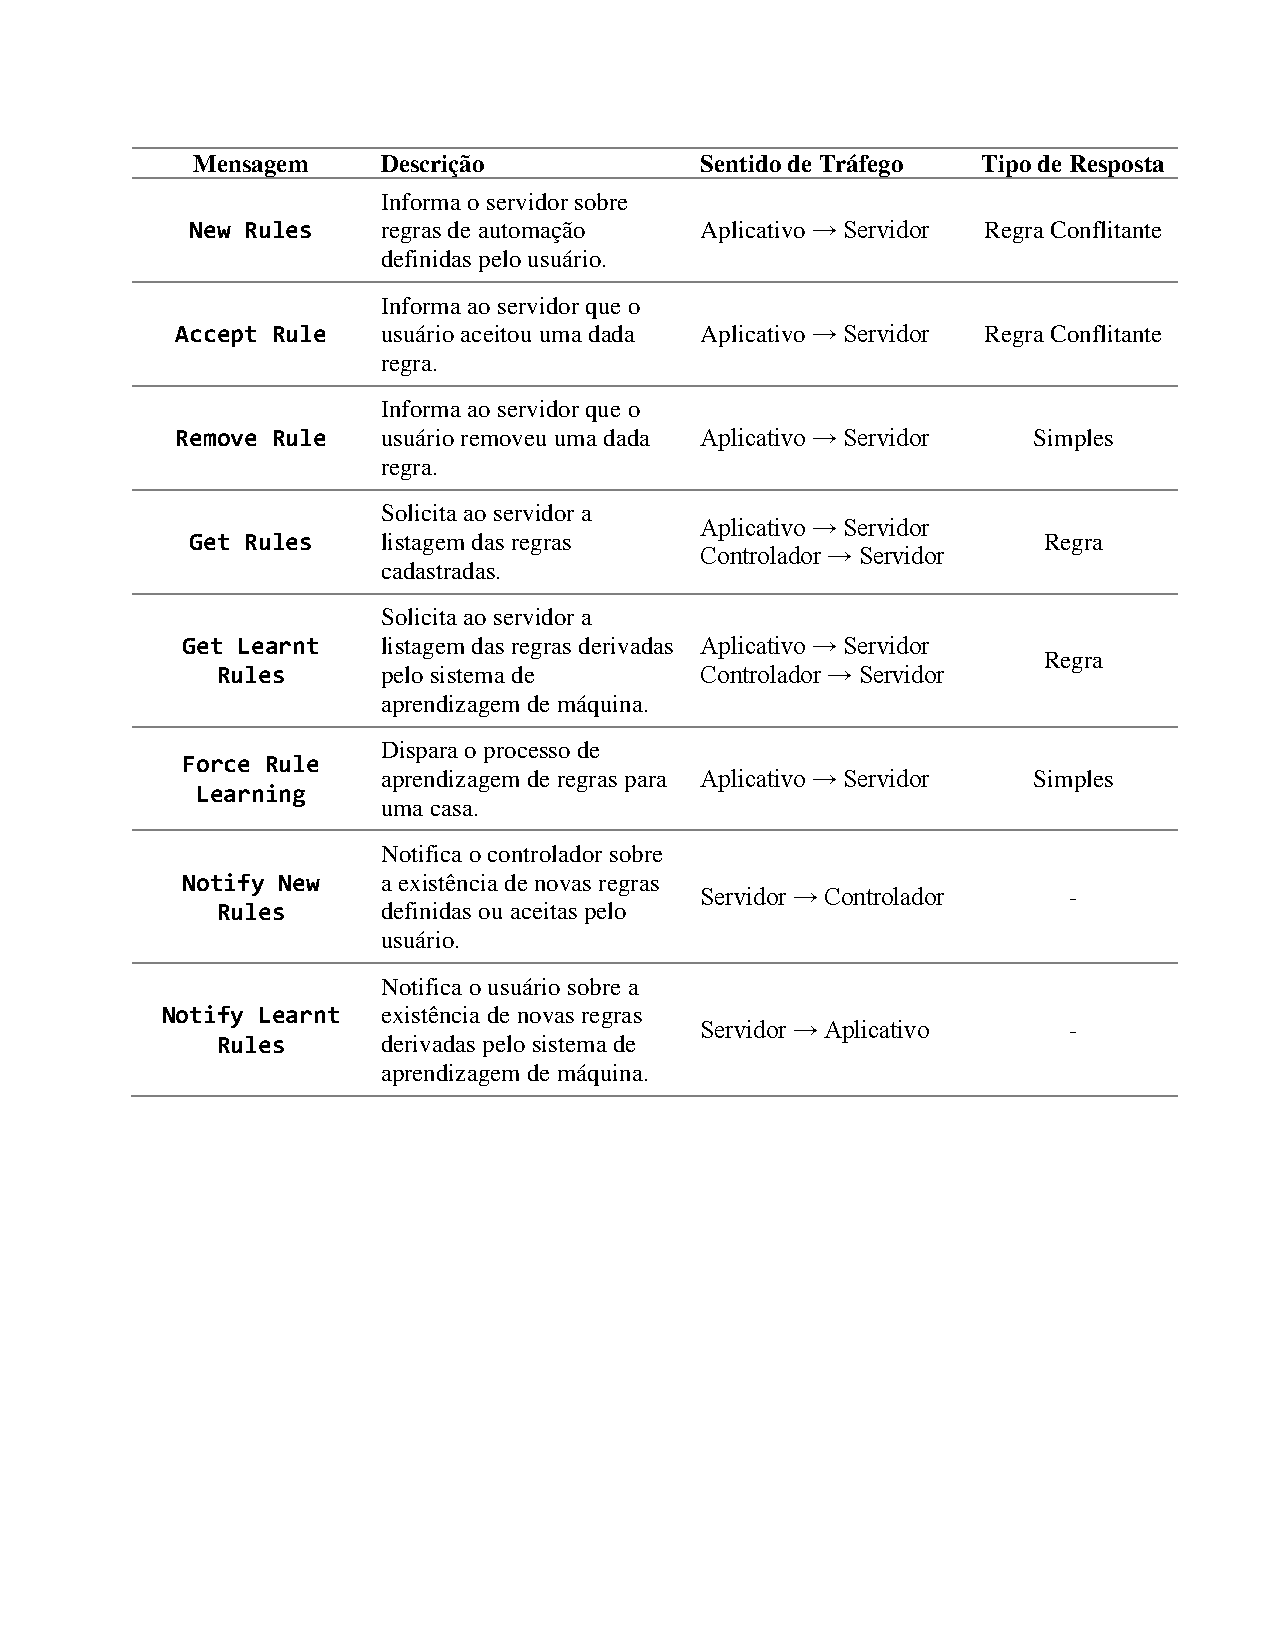
\includegraphics[width=\textwidth]{tabelas/mensagens_regra.pdf}
\end{table}

\paragraph*{\texttt{New Rules}.} A Listagem \ref{lst:newRules} ilustra o formato da mensagem. Uma mensagem deste tipo pode definir diversas regras, declaradas no campo \texttt{rules}. Cada regra especifica o n�-alvo(\texttt{nodeId}), o controlador associado (\texttt{controllerId}), o comando interno do n� (\texttt{commandId}) e o valor que este comando deve assumir (\texttt{value}) caso a condi��o representada pela cl�usula (\texttt{clause}) se mostre verdadeira. Uma cl�usula consiste em uma express�o booleana representada em CNF, codificada, na listagem, como uma lista de listas de proposi��es.

\noindent
\begin{minipage}[l]{\linewidth}
\lstinputlisting[label=lst:newRules, caption=Formato da mensagem \texttt{newRules}]{codigos/newRules.json}
\end{minipage}

\paragraph*{\texttt{Accept Rule}.} A Listagem \ref{lst:acceptRule} ilustra o formato da mensagem. Esta mensagem indica a decis�o do usu�rio em aceitar ou rejeitar a regra explicitada no corpo da mensagem, atrav�s do campo \texttt{accept}.

\noindent
\begin{minipage}[l]{\linewidth}
\lstinputlisting[label=lst:acceptRule, caption=Formato da mensagem \texttt{acceptRule}]{codigos/acceptRule.json}
\end{minipage}

\paragraph*{\texttt{Remove Rule}.} A Listagem \ref{lst:removeRule} ilustra o formato da mensagem. Esta mensagem indica a decis�o do usu�rio em remover uma regra j� cadastrada no sistema (definida ou previamente aceita por ele).

\noindent
\begin{minipage}[l]{\linewidth}
\lstinputlisting[label=lst:removeRule, caption=Formato da mensagem \texttt{removeRule}]{codigos/removeRule.json}
\end{minipage}

\paragraph*{\texttt{Get Rules}.} A Listagem \ref{lst:getRules} ilustra o formato da mensagem.

\noindent
\begin{minipage}[l]{\linewidth}
\lstinputlisting[label=lst:getRules, caption=Formato da mensagem \texttt{getRules}]{codigos/getRules.json}
\end{minipage}

\paragraph*{\texttt{Get Learnt Rules}.} A Listagem \ref{lst:getLearntRules} ilustra o formato da mensagem.

\noindent
\begin{minipage}[l]{\linewidth}
\lstinputlisting[label=lst:getLearntRules, caption=Formato da mensagem \texttt{getLearntRules}]{codigos/getLearntRules.json}
\end{minipage}

\paragraph*{\texttt{Notify New Rules}.} A Listagem \ref{lst:notifyNewRules} ilustra o formato da mensagem. O campo \texttt{quantity} cont�m o n�mero de novas regras dispon�veis para adicionar ao banco de dados do controlador.

\noindent
\begin{minipage}[l]{\linewidth}
\lstinputlisting[label=lst:notifyNewRules, caption=Formato da mensagem \texttt{notifyNewRules}]{codigos/notifyNewRules.json}
\end{minipage}

\paragraph*{\texttt{Notify Learnt Rules}.} A Listagem \ref{lst:notifyLearntRules} ilustra o formato da mensagem. O campo \texttt{quantity} cont�m o n�mero de novas regras dispon�veis para an�lise do usu�rio.

\noindent
\begin{minipage}[l]{\linewidth}
\lstinputlisting[label=lst:notifyLearntRules, caption=Formato da mensagem \texttt{notifyLearntRules}]{codigos/notifyLearntRules.json}
\end{minipage}

\subsubsection{Mensagens de Gerenciamento de N�s}
As mensagens de gerenciamento de n�s est�o listadas e descritas na Tabela \ref{tab:mensagens_nos}.

\begin{table}[hp]
	\centering
	\caption{Listagem e descri��o das Mensagens de Gerenciamento de N�s.}\smallskip
	\label{tab:mensagens_nos}
	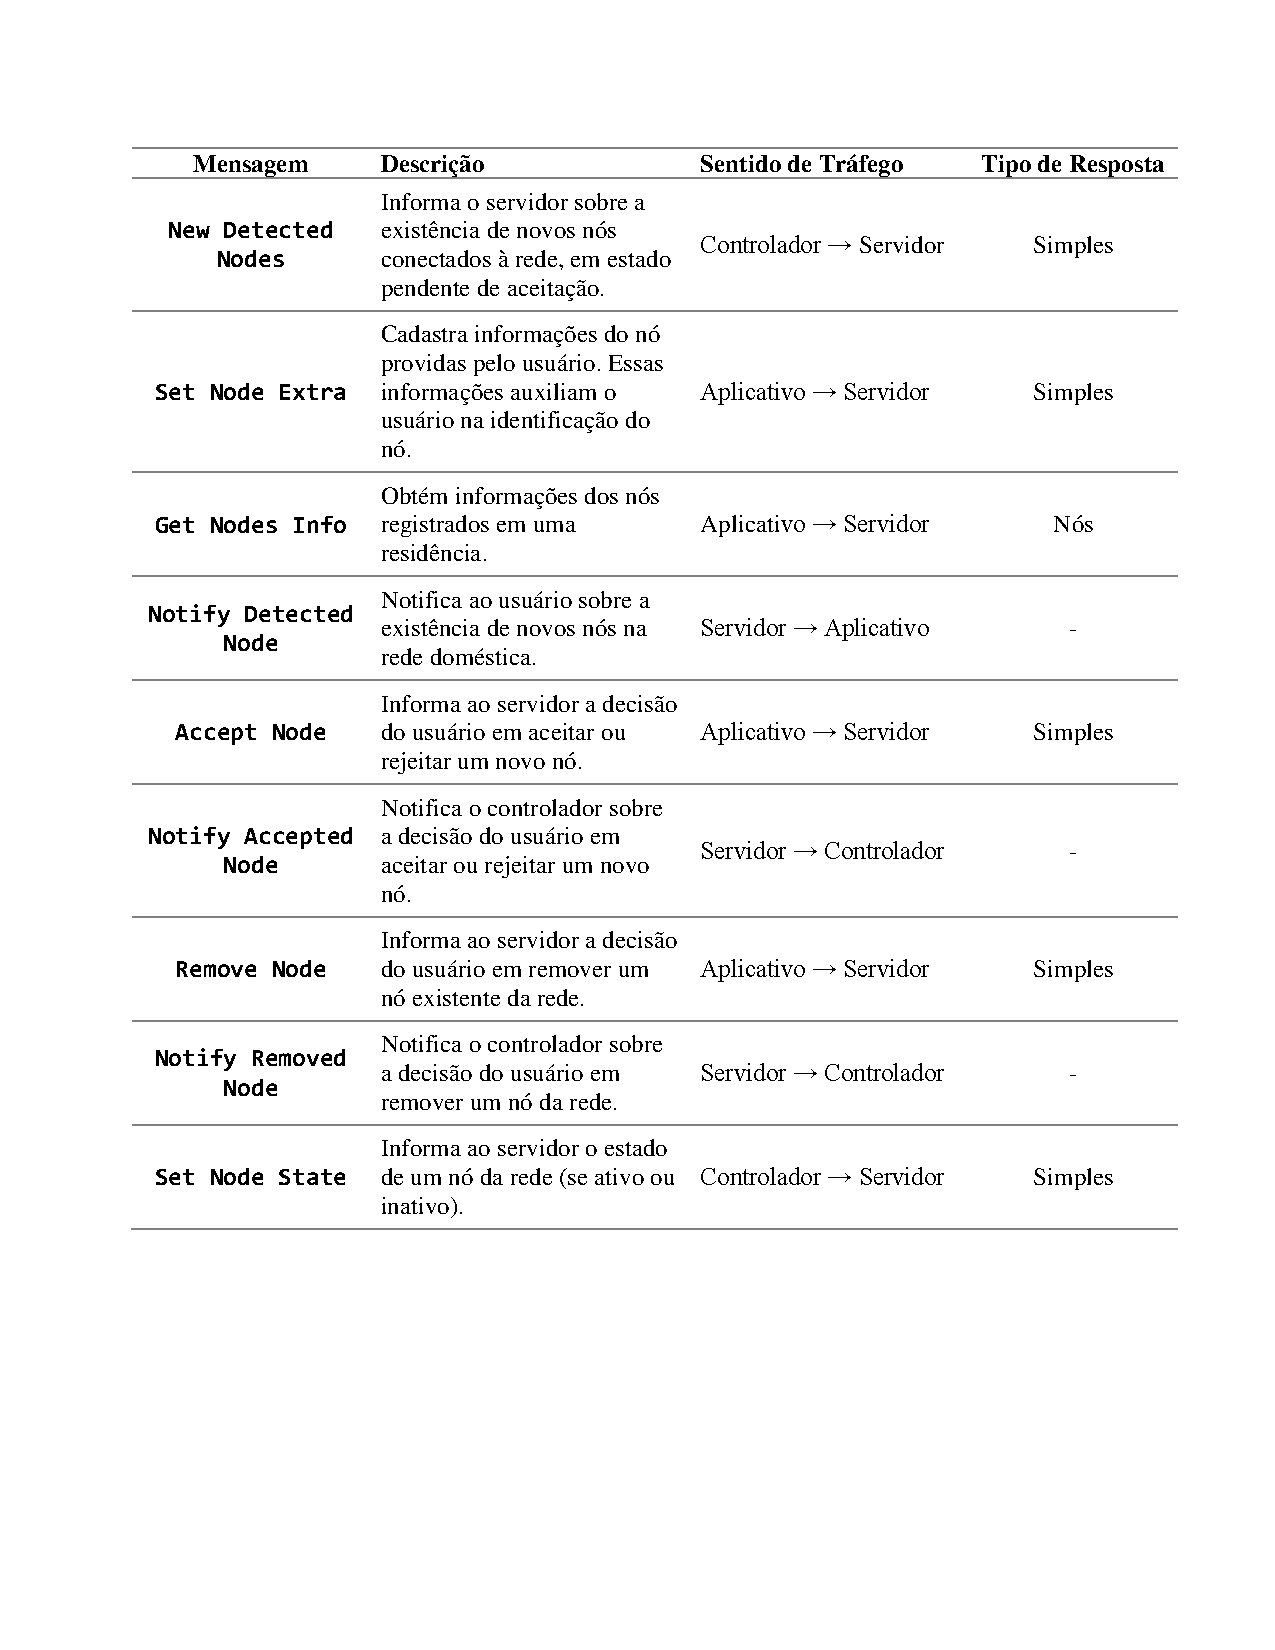
\includegraphics[width=\textwidth]{tabelas/mensagens_nos.pdf}
\end{table}

\paragraph*{\texttt{New Detected Nodes}.} A Listagem \ref{lst:newDetectedNodes} ilustra o formato da mensagem. O campo \texttt{node} cont�m informa��es utilizadas na descri��o do n�, e reflete os campos utilizados nas mensagens de \texttt{description} do protocolo \textit{Rainfall}, definido na \ref{subsec:sintaxe}. Por exemplo, est�o presentes na mensagem o identificador do n� (\texttt{nodeId}), sua classe (\texttt{nodeClass}), informa��es dos dados lidos pelo n� (\texttt{dataType}) bem como dos comandos aceitos por ele (\texttt{commandType}).

\noindent
\begin{minipage}[l]{\linewidth}
\lstinputlisting[label=lst:newDetectedNodes, caption=Formato da mensagem \texttt{newDetectedNodes}]{codigos/newDetectedNodes.json}
\end{minipage}

\paragraph*{\texttt{Set Node Extra}.} A Listagem \ref{lst:setNodeExtra} ilustra o formato da mensagem. Os campos \texttt{nodeId} e \texttt{controllerId} definem o n� para o qual se deseja definir informa��es extras. O campo \texttt{extra}, por sua vez, cont�m as informa��es propriamente ditas. Por exemplo, o mapeamento poderia incluir uma chave "Nome" com valor "Interruptor de luz", atribuindo, assim, um nome a um dado n� da casa.

\noindent
\begin{minipage}[l]{\linewidth}
\lstinputlisting[label=lst:setNodeExtra, caption=Formato da mensagem \texttt{setNodeExtra}]{codigos/setNodeExtra.json}
\end{minipage}

\paragraph*{\texttt{Get Nodes Info}.} A Listagem \ref{lst:getNodesInfo} ilustra o formato da mensagem.

\noindent
\begin{minipage}[l]{\linewidth}
\lstinputlisting[label=lst:getNodesInfo, caption=Formato da mensagem \texttt{getNodesInfo}]{codigos/getNodesInfo.json}
\end{minipage}

\paragraph*{\texttt{Notify Detected Nodes}.} A Listagem \ref{lst:notifyDetectedNode} ilustra o formato da mensagem. O campo \texttt{quantity} cont�m a quantidade de novos n�s na rede.

\noindent
\begin{minipage}[l]{\linewidth}
\lstinputlisting[label=lst:notifyDetectedNode, caption=Formato da mensagem \texttt{notifyDetectedNode}]{codigos/notifyDetectedNode.json}
\end{minipage}

\paragraph*{\texttt{Accept Node}.} A Listagem \ref{lst:acceptNode} ilustra o formato da mensagem. Os campos \texttt{nodeId} e \texttt{controllerId} identificam o n� que ser� aceito ou rejeitado, a depender do valor do campo \texttt{accept}.

\noindent
\begin{minipage}[l]{\linewidth}
\lstinputlisting[label=lst:acceptNode, caption=Formato da mensagem \texttt{acceptNode}]{codigos/acceptNode.json}
\end{minipage}

\paragraph*{\texttt{Notify Accepted Node}.} A Listagem \ref{lst:notifyAcceptedNode} ilustra o formato da mensagem. O campo \texttt{nodeId} identifica o n� que ser� aceito ou rejeitado, a depender do valor do campo \texttt{accept}.

\noindent
\begin{minipage}[l]{\linewidth}
\lstinputlisting[label=lst:notifyAcceptedNode, caption=Formato da mensagem \texttt{notifyAcceptedNode}]{codigos/notifyAcceptedNode.json}
\end{minipage}

\paragraph*{\texttt{Remove Node}.} A Listagem \ref{lst:removeNode} ilustra o formato da mensagem. Os campos \texttt{nodeId} e \texttt{controllerId} identificam o n� que ser� removido.

\noindent
\begin{minipage}[l]{\linewidth}
\lstinputlisting[label=lst:removeNode, caption=Formato da mensagem \texttt{removeNode}]{codigos/removeNode.json}
\end{minipage}

\paragraph*{\texttt{Notify Removed Node}.} A Listagem \ref{lst:notifyRemovedNode} ilustra o formato da mensagem. O campo \texttt{nodeId} identifica o n� que ser� removido.

\noindent
\begin{minipage}[l]{\linewidth}
\lstinputlisting[label=lst:notifyRemovedNode, caption=Formato da mensagem \texttt{notifyRemovedNode}]{codigos/notifyRemovedNode.json}
\end{minipage}

\paragraph*{\texttt{Set Node State}.} A Listagem \ref{lst:setNodeState} ilustra o formato da mensagem. O campo \texttt{nodeId} identifica o n� a que a mensagem se refere, ao passo que o campo \texttt{alive} indica se o n� est� ativo (1) ou n�o (0).

\noindent
\begin{minipage}[l]{\linewidth}
\lstinputlisting[label=lst:setNodeState, caption=Formato da mensagem \texttt{setNodeState}]{codigos/setNodeState.json}
\end{minipage}

\section{Desenvolvimento do Algoritmo de Aprendizagem}
Nesta se��o, detalha-se o processo de desenvolvimento de um algoritmo de aprendizagem para o dom�nio de controle de ilumina��o. O algoritmo recebe como entradas um conjunto de dados descrevendo o estado de sensores e atuadores, provenientes do controlador local, e produz como sa�das regras de atua��o, condicionais aos estados dos sensores.

\subsection{Formato de Entrada dos Dados}\label{subsec:formatoentrada}
No dom�nio selecionado para este trabalho, o dado de atua��o relevante seria o estado da l�mpada a ser controlada. O objetivo do algoritmo, ent�o, � prever o valor deste estado baseado nas leituras de outros sensores existentes na rede dom�stica, tais como de luminosidade e presen�a. A Tabela \ref{tab:entrada_learning} ilustra o formato de entrada dos dados.

\begin{table}[h]
	\centering
	\caption{Formato dos dados de entrada para o algoritmo de aprendizagem.}\smallskip
	\label{tab:entrada_learning}
	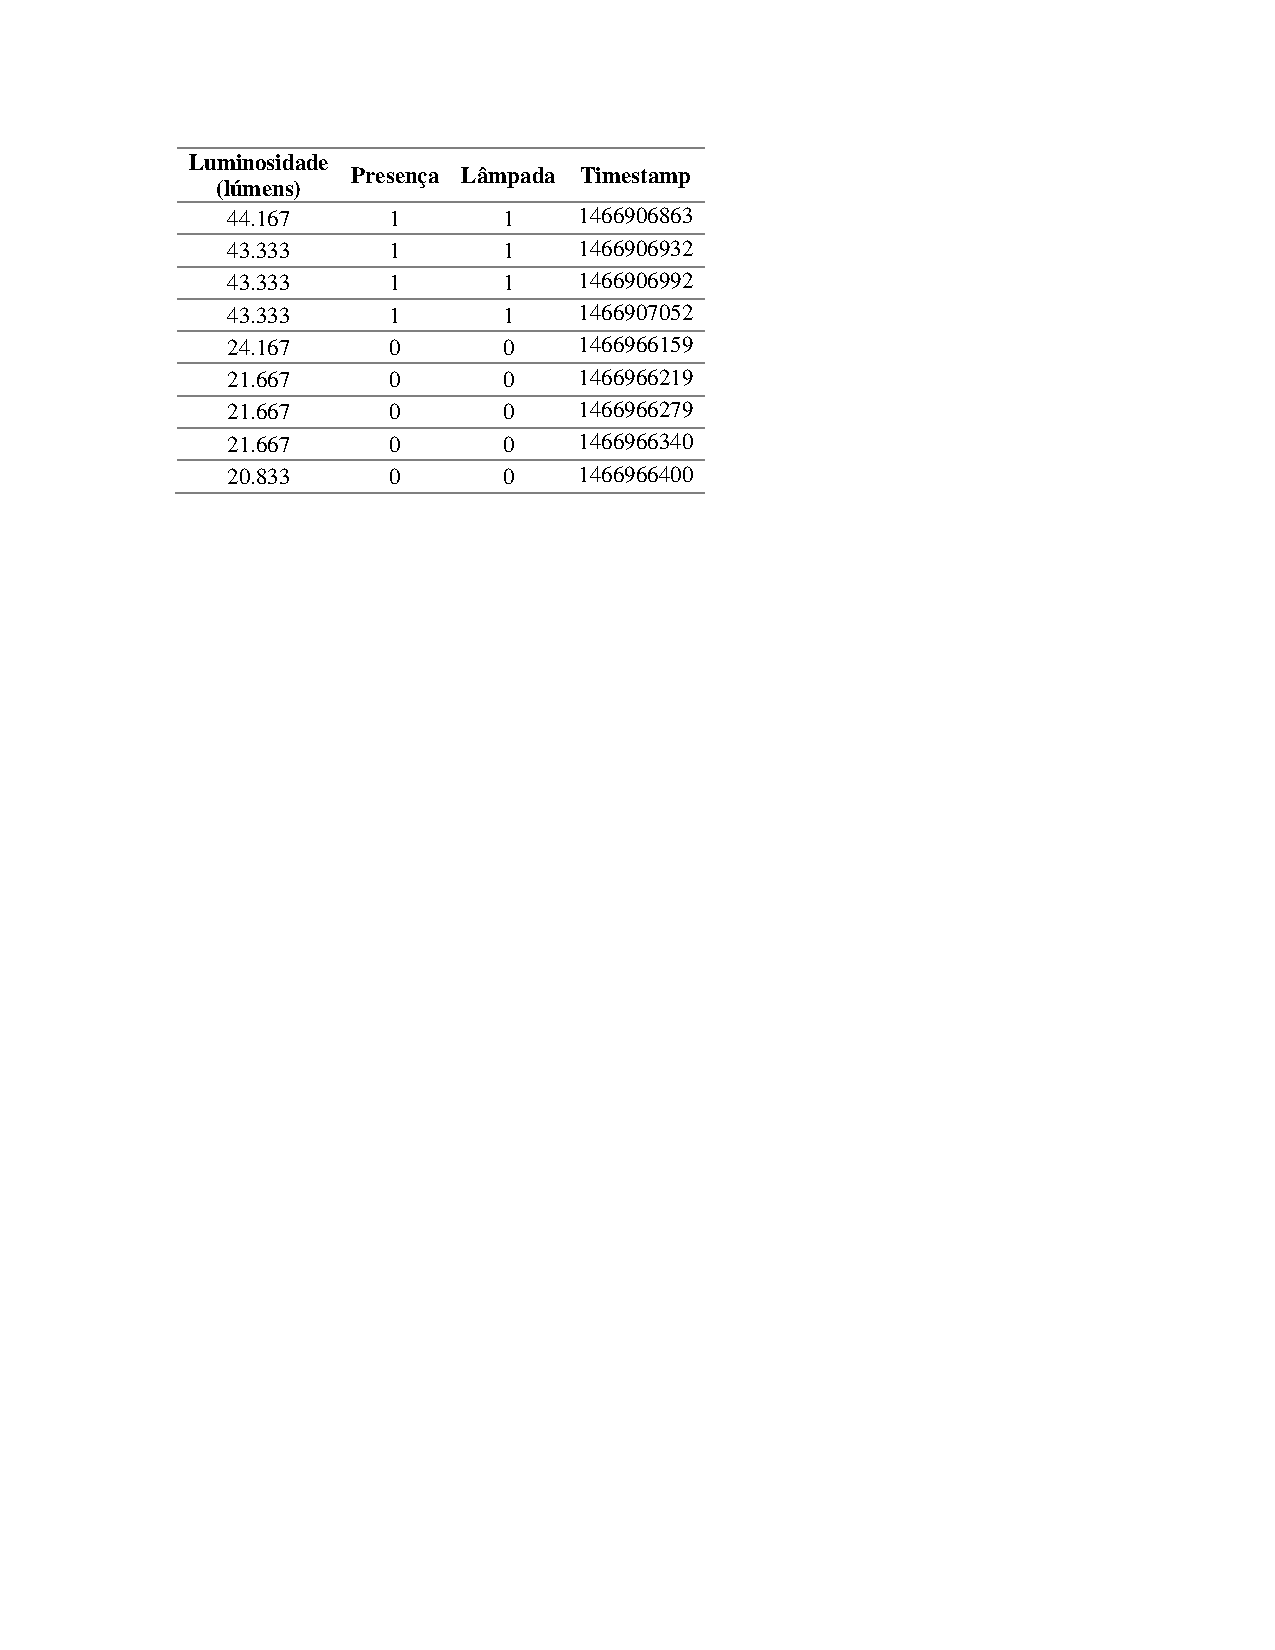
\includegraphics[width=0.5\textwidth]{tabelas/entrada_learning.pdf}
\end{table}

Observe que o problema em quest�o consiste em receber dados de treino, que representam o comportamento do usu�rio, e desenvolver um modelo que preveja o estado do atuador de forma fiel aos dados observados. Trata-se, portanto, de um problema de aprendizagem supervisionada, definido em \cite{james2014} como sendo a gera��o de um modelo que relaciona uma vari�vel-alvo (no caso, o estado da l�mpada) com vari�veis preditoras (presen�a, luminosidade, entre outros). O estado da l�mpada, ent�o, � visto como uma classe associada a cada entrada do conjunto de dados, e o processo de aprendizagem supervisionado que infere esta classe para entradas n�o vistas anteriormente � denominado Classifica��o.

\subsection{Algoritmos de Classifica��o Existentes}\label{subsec:algclass}
Existem diversos algoritmos de classifica��o documentados na literatura, cada qual adotando uma abordagem distinta para gera��o de modelos e classifica��o de dados novos \cite{han2005, james2014}. A seguir ser�o descritos de forma sucinta tr�s t�cnicas candidatas a serem utilizadas no processo de deriva��o de regras para este projeto.

\subsubsection{Indu��o por �rvore de Decis�o}
O modelo de classifica��o gerado por esta t�cnica consiste em uma �rvore de decis�o, em que cada n� interno representa um teste a uma vari�vel preditora, cada aresta representa uma sa�da do teste, e cada n� terminal (folha) indica a classe resultante. A Figura \ref{fig:exemplo_arvore} mostra o exemplo de uma �rvore de decis�o obtida por esta t�cnica. 

Neste exemplo, o conjunto de dados refere-se a consumidores de uma loja de eletr�nicos, e as classes mostradas nos n�s-folha indicam se um consumidor adquire ou n�o certo produto. No caso, uma das regras geradas pelo modelo diz que se o consumidor � jovem e estudante, ent�o ele adquire o produto.

\begin{figure}[h]
	\centering
	\caption{Exemplo de modelo gerado pela t�cnica de Indu��o por �rvore de Decis�o}
  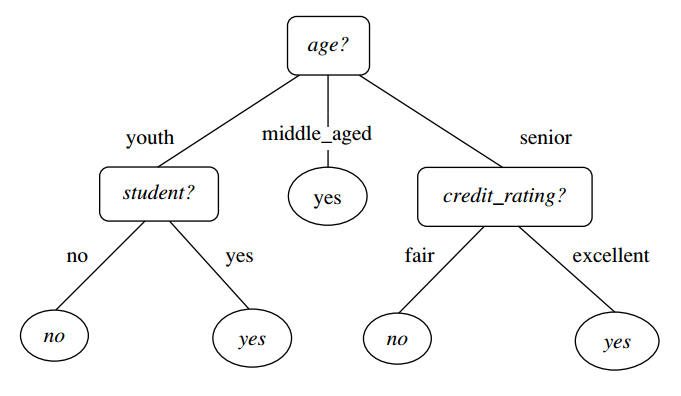
\includegraphics[width=0.8\textwidth]{imagens/exemplo_arvore.png}
  \label{fig:exemplo_arvore}  
  
  Fonte: \cite{han2005}
\end{figure}

Existem diversas implementa��es desta t�cnica de classifica��o, tais como ID3, C4.5 e CART, que adotam uma estrat�gia \textit{greedy} e \textit{top-down} de constru��o da �rvore. Cada uma dessas implementa��es efetua o particionamento dos dados de forma particular, efetuando sele��o de vari�veis por crit�rios tais como ganho de informa��o, raz�o de ganho ou �ndice Gini. As descri��es dessas t�cnicas fogem do escopo deste trabalho, e podem ser encontradas em \cite{han2005}.

\subsubsection{Redes Neurais}
A t�cnica de aprendizagem por redes neurais foi inspirada pelos ramos da psicologia e neurobiologia, que buscaram modelar computacionalmente o comportamento de neur�nios. Uma rede neural � composta por diversas unidades interconectadas arranjadas em camadas, conforme ilustra a Figura \ref{fig:elem_rede_neural}. 

Os dados de entrada do classificador s�o passados para as unidades da camada de entrada. Esses dados, ent�o, s�o combinados linearmente atrav�s de pesos determinados nas interconex�es e passados �s unidades das camadas intermedi�rias, denominadas \textit{hidden layers}. As sa�das da �ltima camada intermedi�ria s�o passadas �s unidades da camada de sa�da, que define a classe resultante.

\begin{figure}[h]
	\centering
	\caption{Elementos de uma rede neural}
  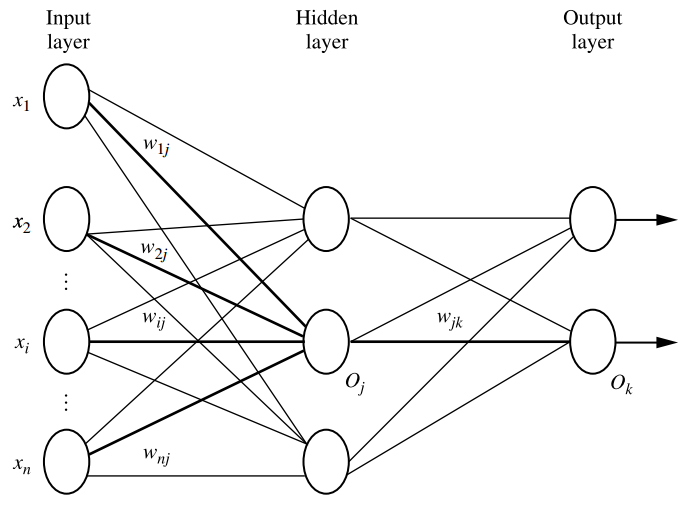
\includegraphics[width=0.8\textwidth]{imagens/elem_rede_neural.png}
  \label{fig:elem_rede_neural}  
  
  Fonte: \cite{han2005}
\end{figure}

O processo de aprendizagem das redes neurais � computacionalmente caro e complexo, envolvendo um processo denominado \textit{backpropagation}. Este � um processo iterativo que consiste em alimentar os dados de treino na rede neural, obter a sa�da com o modelo corrente, e reajustar os pesos do modelo em ordem reversa, partindo das unidades da camada de sa�da.

No entanto, as redes neurais possuem a vantagem de possu�rem alta toler�ncia a dados ruidosos, al�m de n�o requerer conhecimento da rela��o entre as classes a serem previstas e as vari�veis preditoras \cite{han2005}.

\subsubsection{\textit{Support Vector Machines} (SVM)}
O SVM � uma t�cnica de classifica��o que se baseia na defini��o de um hiperplano �timo para efetuar a segrega��o dos dados pertencentes �s diferentes classes. No caso, o hiperplano �timo seria o que prov� maior margem entre os dados, conforme ilustra a Figura \ref{fig:svm_max_margin}. Neste exemplo, o conjunto de dados � bidimensional, e o hiperplano de separa��o � uma reta. Observe que das diversas retas poss�veis mostradas � esquerda, seleciona-se a que resulta em maior margem, mostrada � direita.

\begin{figure}[h]
	\centering
	\caption{Retas candidatas para efetuar a segrega��o dos dados (esq.), e a reta �tima selecionada, que prov� a maior margem no conjunto de dados}
  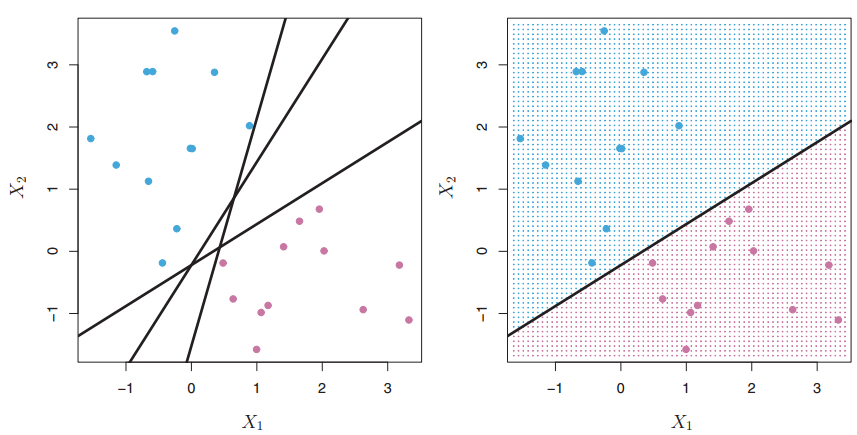
\includegraphics[width=0.8\textwidth]{imagens/svm_max_margin.png}
  \label{fig:svm_max_margin}  
  
  Fonte: \cite{james2014}
\end{figure}

A t�cnica de SVM se baseia nesta ideia de definir um plano de separa��o �timo, mas efetua a adi��o de mais dimens�es aos dados originais para lidar com situa��es de margens n�o-lineares. Este aumento na dimensionalidade dos dados � feito com base na utiliza��o de \textit{kernels}. A descri��o matem�tica deste processo est� fora do escopo deste trabalho, e pode ser encontrado em \cite{james2014}.

\subsection{Considera��es sobre a Escolha do Algoritmo}
A se��o \ref{subsec:algclass} apresentou tr�s algoritmos de classifica��o pass�veis de serem aplicados no projeto. Conforme mencionado, cada algoritmo possui uma abordagem distinta na constru��o do modelo e na avalia��o de entradas novas para efetuar a classifica��o, possuindo vantagens e desvantagens particulares. Esta se��o lista as considera��es adotadas para a sele��o do algoritmo a ser utilizado na gera��o de regras.

O fator principal utilizado para selecionar o algoritmo de aprendizagem � a interpretabilidade do modelo gerado. Dentre as raz�es para a prioriza��o deste fator, destaca-se a necessidade de o usu�rio ter capacidade de analisar as regras propostas pelo algoritmo, de modo a dar-lhe a escolha de aceit�-la ou recus�-la. Essa possibilidade � extremamente importante, levando-se em conta que os sensores utilizados em ambiente dom�stico podem possuir imprecis�es que resultem na gera��o de regras estatisticamente precisas, mas ainda assim indesejadas pelo usu�rio.

Nesse contexto, \cite{james2014} menciona haver um \textit{tradeoff} entre a flexibilidade e a interpretabilidade dos m�todos de aprendizagem, como mostra a Figura \ref{fig:interpretabilidade_algoritmos}. M�todos flex�veis possuem alta capacidade de gerar modelos que se adaptem a dados de natureza complexa, mas tais modelos acabam sendo de dif�cil interpreta��o pelo usu�rio. 

\begin{figure}[h]
	\centering
	\caption{\textit{Tradeoff} entre flexibilidade e interpretabilidade de m�todos de aprendizagem}
  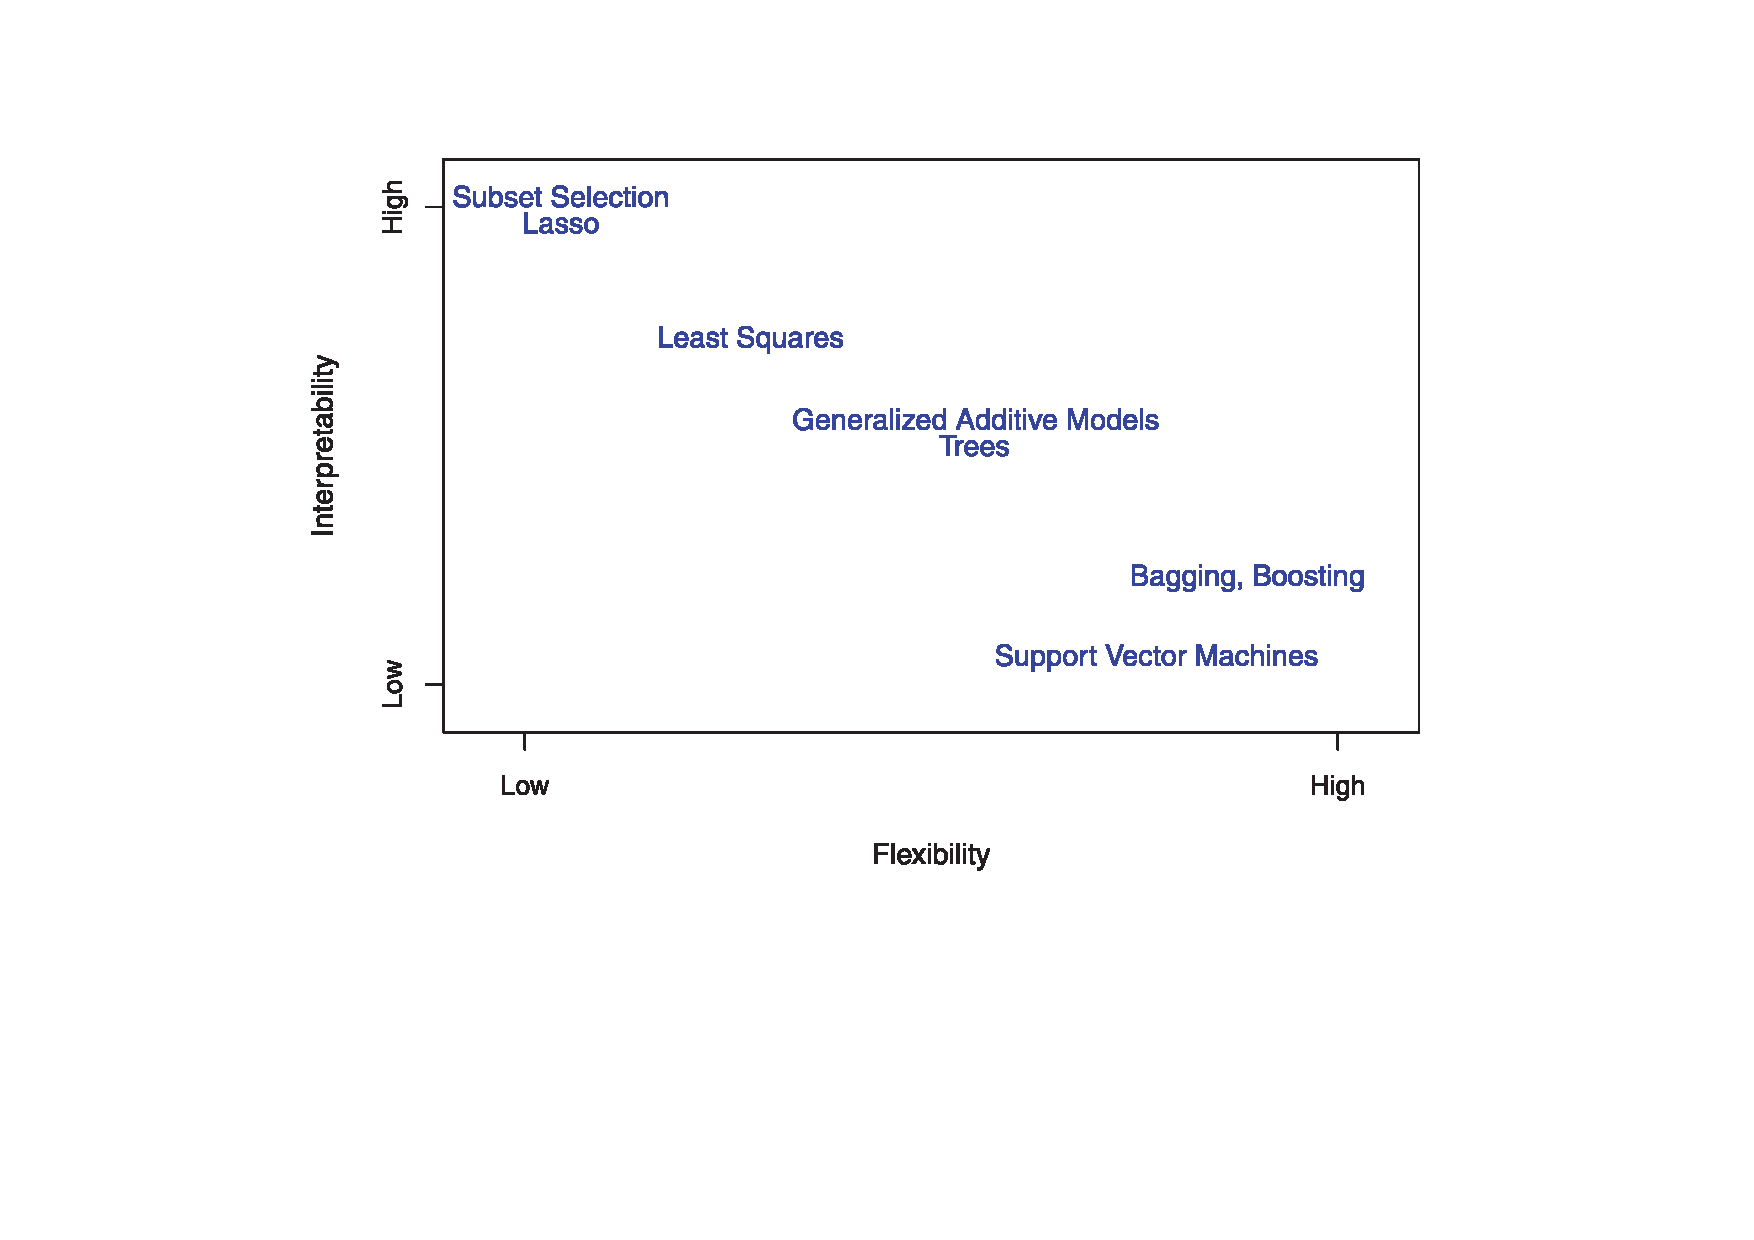
\includegraphics[width=0.8\textwidth]{imagens/interpretabilidade_algoritmos.pdf}
  \label{fig:interpretabilidade_algoritmos}  
  
  Fonte: \cite{james2014}
\end{figure}

Note que, dentre as t�cnicas apresentadas, redes neurais e SVM possuem alta flexibilidade, permitindo gerar modelos para dados com vari�veis cuja rela��o � desconhecida, a princ�pio (no caso das redes neurais), e para dados com fronteira de decis�o n�o-linear (no caso do SVM). Entretanto, os modelos gerados por estas t�cnicas s�o pouco interpret�veis: redes neurais exp�em um conjunto de pesos que processam os dados, de acordo com a topologia selecionada, e o SVM gera um hiperplano de separa��o.

No extremo oposto encontra-se a t�cnica de classifica��o por �rvores de decis�o. Este m�todo � mais restritivo em termos de flexibilidade, mas gera modelos facilmente interpret�veis. De posse de um modelo como o da Figura \ref{fig:exemplo_arvore}, por exemplo, � intuitivo obter os fatores que influenciam na classifica��o das entradas.

Pelas raz�es mencionadas anteriormente, o algoritmo de classifica��o por �rvore de decis�o foi adotado para derivar regras de atua��o. A seguir ser�o descritos os experimentos feitos com  dados de ilumina��o, englobando o preprocessamento dos dados e a aplica��o do algoritmo de classifica��o propriamente dito.

\subsection{Coleta de Dados}
Conforme mencionado, o dom�nio de aplica��o abordado para concep��o de um algoritmo de aprendizagem de regras � o de controle de ilumina��o. Para iniciar os testes, � necess�rio ter em m�os um \textit{dataset} em formato similar ao descrito na se��o \ref{subsec:formatoentrada}. Para obter tais dados de treino, os membros do grupo adquiriram sensores de presen�a PIR e de ilumina��o, associando-os a um Raspberry Pi, a fim de coletar dados nas respectivas resid�ncias. A Figura \ref{fig:montagem_coleta} mostra as montagens utilizadas para efetuar as coletas nas resid�ncias.

\begin{figure}[h]
	\centering
	\caption{Montagens experimentais para coleta de dados de ilumina��o}
	\smallskip
  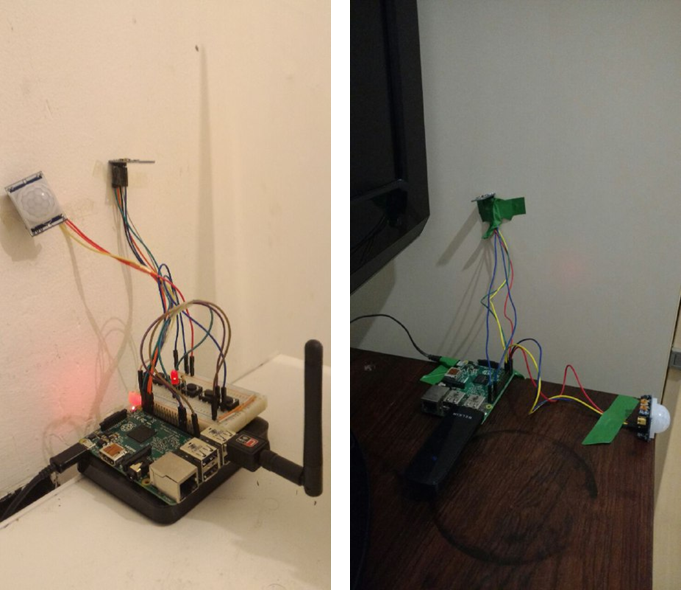
\includegraphics[width=0.8\textwidth]{imagens/montagem_coleta.png}
  \label{fig:montagem_coleta}  
\end{figure}

Neste processo, os dados foram amostrados a cada minuto. Na primeira montagem, foi utilizado um bot�o para sinalizar o momento em que o interruptor foi acionado, devido � inviabilidade de conectar o interruptor existente no processo de coleta. Os dados coletados por esta montagem ser�o referidos por \textit{dataset} 1. Na segunda montagem, o estado do interruptor foi inferido posteriormente, de acordo com o hor�rio do dia e da ilumina��o ambiente. Os dados coletados por esta montagem ser�o denominados \textit{dataset} 2. O \textit{timestamp}, mostrado na Tabela \ref{tab:entrada_learning}, foi registrado para cada amostra coletada, e consiste na representa��o POSIX do instante de coleta do dado.

\subsection{Experimentos para Deriva��o de Regras}
Como mencionado, o grupo pretende usar um algoritmo de classifica��o baseado em �rvore de decis�o para gerar as regras de atua��o. Levando em conta a rotina associada aos dados de treino coletados, o grupo espera, idealmente, que as seguintes regras sejam derivadas:
\begin{itemize}
	\item Acenda a luz quando h� algu�m no ambiente, e a ilumina��o no local � baixa;
	\item Apague a luz quando n�o h� ningu�m no ambiente
\end{itemize}

Para a gera��o das �rvores de decis�o, o grupo usou a ferramenta Rattle\footnote{Dispon�vel em \url{http://rattle.togaware.com/}.}, que utiliza um algoritmo recursivo \textit{top-down} \cite{williams2011} implementado na biblioteca \texttt{rpart}\footnote{Documenta��o dispon�vel em \url{https://cran.r-project.org/web/packages/rpart/index.html}}. O objetivo, nesta se��o, � estudar modos de preprocessamento dos dados utilizados pelo algoritmo, e analisar a qualidade das regras criadas. Todo o processamento efetuado sobre os dados foi feito utilizando a linguagem R\footnote{Dispon�vel em \url{https://www.r-project.org/}}.

\subsubsection{Utiliza��o de dados \textit{raw}}
A primeira tentativa de gera��o de regras foi feita alimentando o algoritmo de gera��o do modelo sem efetuar nenhum tipo de preprocessamento dos dados. Os resultados obtidos est�o apresentados na Figura \ref{fig:teste_1}, para cada \textit{dataset} utilizado. Para auxiliar na interpretabilidade dos dados, tenha em mente que valores de lumin�ncia na ordem de 40 lx correspondem a um ambiente noturno, com uma l�mpada acesa.

\begin{figure}[hp]
	\caption{�rvores de decis�o geradas sem nenhum preprocessamento de dados.}
	\smallskip
	\begin{subfigure}{\textwidth}
		\centering
  	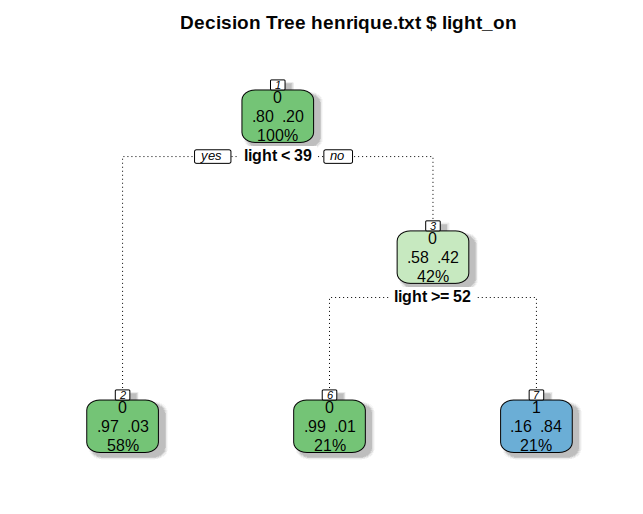
\includegraphics[width=0.8\textwidth]{imagens/teste_learning/1_h.png}
  \end{subfigure}
  	\begin{subfigure}{\textwidth}
		\centering
  	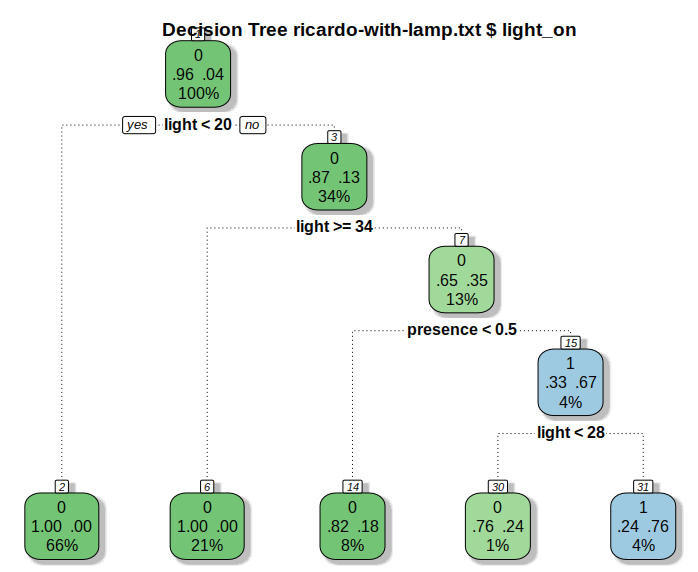
\includegraphics[width=0.8\textwidth]{imagens/teste_learning/1_r.png}
  \end{subfigure}
  \label{fig:teste_1}  
\end{figure}

Observe que, no primeiro caso, o algoritmo tenta prever o estado da l�mpada baseado unicamente nos dados de ilumina��o ambiente, ao passo que no segundo, dados de presen�a tamb�m s�o utilizados. No entanto, a partir das regras criadas, � evidente que o algoritmo est� prevendo qual o estado corrente da l�mpada, dados os par�metros de entrada de lumin�ncia e presen�a. Por exemplo, uma das regras criadas diz que se o n�vel de luminosidade do ambiente for menor que 39, ent�o a l�mpada est� apagada.

Para fins de cria��o de regras, o interesse maior est� em identificar o estado em que ocorreu uma mudan�a no estado da l�mpada. Para tanto, torna-se necess�rio efetuar um preprocessamento dos dados para evidenciar essas mudan�as no \textit{dataset}.

\subsubsection{Adi��o de um campo de A��o}
Nesta tentativa, foi efetuado um passo de preprocessamento adicionando uma coluna indicando a a��o tomada no instante. Por exemplo, se em um dado instante a l�mpada est� apagada, mas no seguinte ela est� acesa, ent�o o campo "A��o" assume valor "1", indicando que a l�mpada foi acesa. Analogamente, se a l�mpada est� acesa em um dado instante e no seguinte ela est� apagada, ent�o o campo "A��o" assume valor "-1", indicando que ela foi apagada. Caso o estado da l�mpada seja o mesmo em dois instantes de tempo consecutivos, o campo "A��o" assume valor "0", indicando aus�ncia de a��o.

Efetuando este tratamento, o algoritmo n�o produziu nenhum resultado, n�o sendo capaz de criar regras em ambos os \textit{datasets}. Uma an�lise mais profunda mostrou a raz�o disso: o n�mero de pontos em que n�o houve a��o � ordens de grandeza maior do que os pontos em que houve a��o (cerca de 400 vezes mais pontos no primeiro dataset, e 300 no segundo). 

\subsubsection{Elimina��o dos pontos sem a��o} \label{subsubsec:elim_pts_sem_acao}
Esta tentativa buscou explorar a efic�cia do algoritmo caso pontos sem a��o (A��o=0) fossem eliminados. A Figura \ref{fig:teste_3} mostra as �rvores de decis�o geradas nesta tentativa.

\begin{figure}[hp]
	\caption{�rvores de decis�o geradas mantendo somente pontos com a��o tomada.}
	\smallskip
	\begin{subfigure}{\textwidth}
		\centering
  	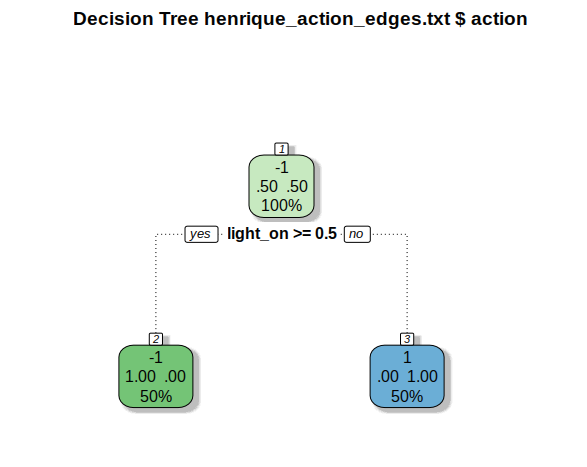
\includegraphics[width=0.8\textwidth]{imagens/teste_learning/3_h.png}
  \end{subfigure}
  	\begin{subfigure}{\textwidth}
		\centering
  	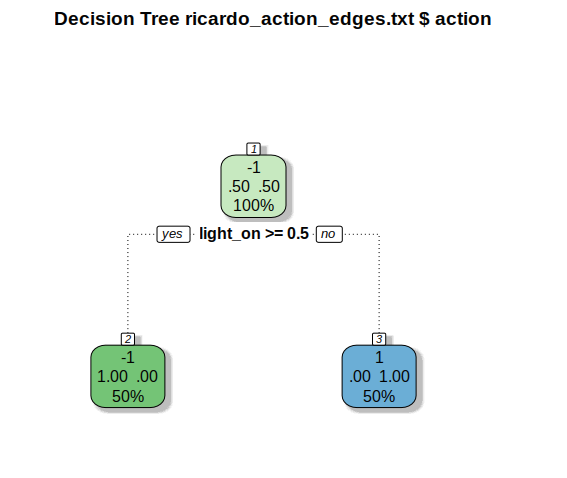
\includegraphics[width=0.8\textwidth]{imagens/teste_learning/3_r.png}
  \end{subfigure}
  \label{fig:teste_3}  
\end{figure}

Observe que as regras geradas ditam que a luz seja apagada, caso ela esteja acesa, e vice-versa. De fato, do universo de pontos coletados neste item, � �bvio que a luz sempre � apagada quando ela est� acesa, e ela sempre � acesa quando est� apagada. Ocorre que a elimina��o dos dados de A��o=0, apesar de resolver o problema de desbalanceamento, introduziu uma perda de informa��o significativa. Ocorre que, em diversos momentos em que a luz est� acesa, ela n�o � apagada. A manuten��o de tais pontos, pois, se mostra imprescind�vel para a gera��o de regras coerentes.

\subsubsection{Balanceamento do \textit{dataset}}
Conforme mencionado, o \textit{dataset} em quest�o � extremamente desbalanceado, com uma quantidade de entradas com classe A��o=0 ordens de grandeza maior que entradas das demais classes. Conforme mencionado em \cite{han2005}, dentre as t�cnicas utilizadas para se lidar com problemas de classifica��o desbalanceados est�o o \textit{undersampling} da classe majorit�ria e o \textit{oversampling} da classe minorit�ria. Neste teste, a primeira t�cnica ser� adotada para reduzir a quantidade de entradas da classe A��o=0.

O \textit{undersample} foi efetuado selecionando-se uma quantidade de pontos da classe majorit�ria de forma aleat�ria. A Figura \ref{fig:teste_4} mostra as �rvores de decis�o geradas nesta tentativa.

\begin{figure}[hp]
	\caption{�rvores de decis�o geradas efetuando \textit{undersample} da classe majorit�ria.}
	\smallskip
	\begin{subfigure}{\textwidth}
		\centering
  	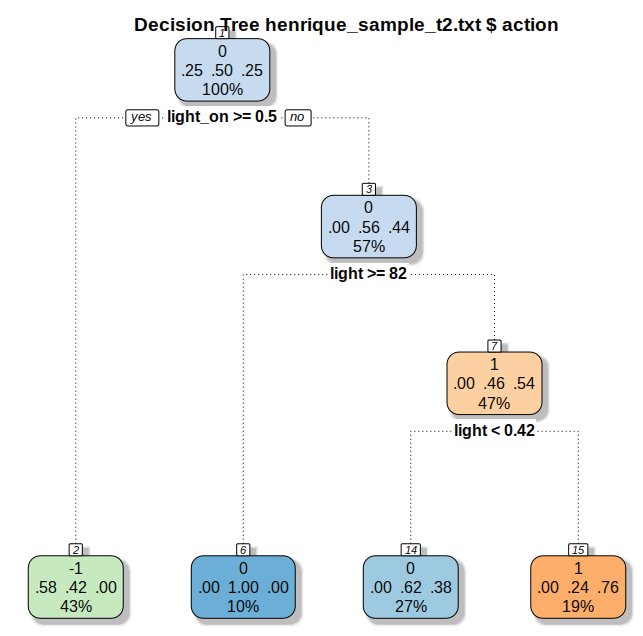
\includegraphics[width=0.8\textwidth]{imagens/teste_learning/4_h.png}
  \end{subfigure}
  	\begin{subfigure}{\textwidth}
		\centering
  	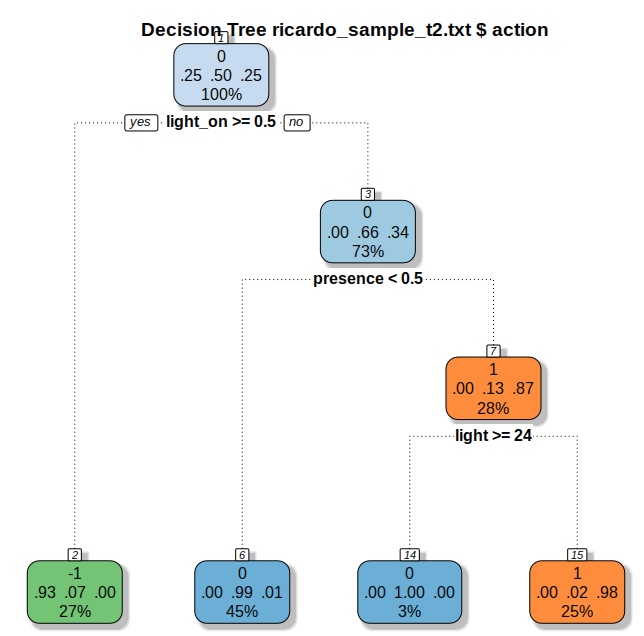
\includegraphics[width=0.8\textwidth]{imagens/teste_learning/4_r.png}
  \end{subfigure}
  \label{fig:teste_4}  
\end{figure}

No \textit{dataset} 1, as regras produzidas foram:
\begin{itemize}
	\item Apague a luz quando ela estiver acesa ($light\_on >= 0.5$)
	\item Acenda a luz quando ela estiver apagada e a ilumina��o ambiente estiver entre 0.42 e 82
	\item N�o fa�a nada caso contr�rio
\end{itemize}
No caso do segundo \textit{dataset}, as regras produzidas foram:
\begin{itemize}
	\item Apague a luz quando ela estiver acesa ($light\_on >= 0.5$)
	\item Acenda a luz quando ela estiver apagada, algu�m estiver no quarto e a ilumina��o ambiente for menor que 24
	\item N�o fa�a nada, caso contr�rio
\end{itemize}

Como foi efetuado uma amostragem aleat�ria em todos os pontos de n�o a��o, reproduzimos esse teste diversas vezes, e as �rvores resultantes s�o as que ocorriam com mais frequ�ncia nos testes. Em ambas as �rvores, observa-se que ele derivou a regra para apagar a luz sempre que ela esteja acesa, e apenas no segundo \textit{dataset} utilizou a presen�a no caso de acender a luz.

Analisando o \textit{dataset}, observa-se que acontece de o usu�rio acender a luz antes da presen�a ser detectada e tamb�m de apag�-la ainda sob alcance do sensor de presen�a. Ou seja, o usu�rio deixa o ambiente quando apaga a luz e o frequenta quando a acende, e essa informa��o n�o � representada tomando unicamente a leitura instant�nea do sensor de presen�a.

\subsubsection{Considera��o de m�dias temporais dos dados}
Com o intuito de capturar o estado do ambiente associado � tomada de uma a��o, testou-se a utiliza��o de uma m�dia temporal de $n$ pontos para a presen�a, em vez de utilizar uma �nica medida instant�nea. Deste modo, para um dado instante, o valor da presen�a � a m�dia dos $n$ valores subsequentes, arranjados de forma temporal. Efetuar este tipo de processamento faz com que os \textit{datasets} reflitam o estado do ambiente ap�s a tomada da a��o, contribuindo para a gera��o de regras mais precisas. No entanto, h� a necessidade de se conhecer a natureza dos dados coletados para que este tipo de processamento fa�a sentido, tornando este tratamento espec�fico para a aplica��o descrita de controle de ilumina��o.

A Figura \ref{fig:teste_5_1} mostra �rvores de decis�o geradas para o \textit{dataset} 1, ao passo que a Figura \ref{fig:teste_5_2} mostra as geradas para o \textit{dataset} 2. Nestes modelos, foi utilizado $n=10$. Devido � natureza aleat�ria do \textit{undersampling}, as duas �rvores apresentadas em cada figura foram geradas frequentemente.

\begin{figure}[hp]
	\caption{�rvores de decis�o geradas para o \textit{dataset} 1 tomando a m�dia temporal da presen�a, com $n=10$.}
	\smallskip
	\begin{subfigure}{\textwidth}
		\centering
  	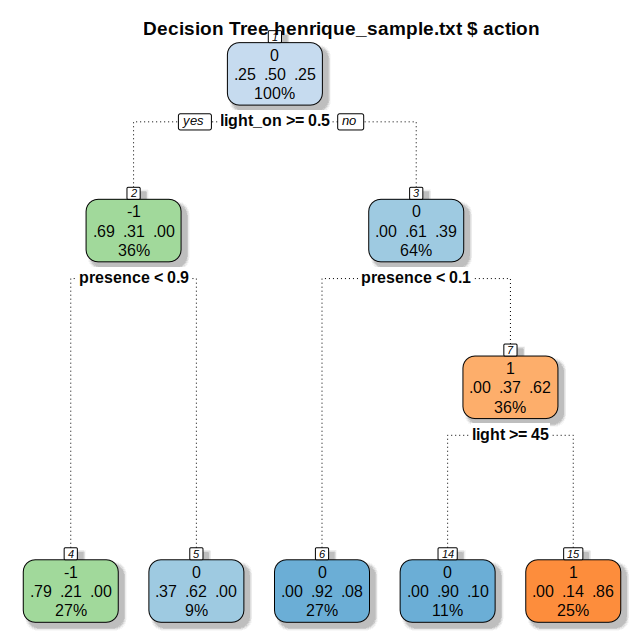
\includegraphics[width=0.8\textwidth]{imagens/teste_learning/5_h_1.png}
  \end{subfigure}
  	\begin{subfigure}{\textwidth}
		\centering
  	\includegraphics[width=0.8\textwidth]{imagens/teste_learning/5_h_2.png}
  \end{subfigure}
  \label{fig:teste_5_1}  
\end{figure}

\begin{figure}[hp]
	\caption{�rvores de decis�o geradas para o \textit{dataset} 2 tomando a m�dia temporal da presen�a, com $n=10$.}
	\smallskip
	\begin{subfigure}{\textwidth}
		\centering
  	\includegraphics[width=0.8\textwidth]{imagens/teste_learning/5_r_1.png}
  \end{subfigure}
  	\begin{subfigure}{\textwidth}
		\centering
  	\includegraphics[width=0.8\textwidth]{imagens/teste_learning/5_r_2.png}
  \end{subfigure}
  \label{fig:teste_5_2}  
\end{figure}

Observe que os resultados obtidos s�o similares para os dois \textit{datasets}. Analisando a primeira �rvore da Figura \ref{fig:teste_5_1}, observa-se que as regras geradas foram:
\begin{itemize}
	\item Apague a luz quando ela estiver acesa e n�o houver ningu�m no ambiente;
	\item Acenda a luz quando ela estiver apagada, houver presen�a no ambiente e o n�vel de luminosidade for menor que 45;
	\item N�o fa�a nada caso contr�rio.
\end{itemize}
No caso da segunda �rvore da Figura \ref{fig:teste_5_1}, tem-se as regras:
\begin{itemize}
	\item Apague a luz quando ela estiver acesa;
	\item Acenda a luz quando ela estiver apagada, houver presen�a no ambiente e o n�vel de luminosidade for menor que 73;
	\item N�o fa�a nada caso contr�rio.
\end{itemize}

Observe que a primeira �rvore obtida gerou regras �timas, levando em conta os \textit{datasets} utilizados. A segunda, no entanto, ainda sugeria regras que simplesmente apagavam a luz quando ela estivesse acesa. Este problema � similar ao obtido no teste \ref{subsubsec:elim_pts_sem_acao}, e provavelmente se deve ao fato de n�o terem sido escolhidos pontos suficientes da classe A��o=0 no processo de \textit{undersampling}.

\subsubsection{\textit{Undersampling} com clusteriza��o}
Uma maneira de melhorar o processo de \textit{undersampling}, de modo que os dados coletados representem mais fielmente o \textit{dataset} original, seria aplicar t�cnicas de clusteriza��o � classe majorit�ria. Desse modo, o procedimento de amostragem consistiria em coletar alguns pontos de cada cluster identificado.

O algoritmo de clusteriza��o utilizado nesta etapa foi o CLARA (\textit{Clustering LARge Applications}), que � classificado como um algoritmo de clusteriza��o por particionamento \cite{han2005}. O CLARA � resultado de uma s�rie de incrementos efetuados sobre outros algoritmos de particionamento, partindo do mais simples: o \textit{k-means}.

O \textit{k-means} � um algoritmo de clusteriza��o iterativo que utiliza a no��o de centroides como pontos representativos de um cluster. Um centroide pode ser visto como o centro geom�trico de um \textit{dataset}. Os clusters s�o definidos da seguinte forma. Seja $C=\{c_1,c_2,...,c_k\}$ o conjunto de pontos representativos (centroides), onde $k$ � o n�mero de clusters, e $dist(x,y)$ uma fun��o de c�lculo de dist�ncia entre dois pontos (por exemplo, dist�ncia euclidiana). Para cada ponto $p$ do \textit{dataset}, $p$ � alocado ao cluster correspondente ao centroide $c_i$ que minimize $dist(p,c_i)$. 

Inicialmente, os $k$ centroides s�o escolhidos de forma aleat�ria do \textit{dataset}. Ent�o, o algoritmo efetua dois passos de forma iterativa:
\begin{enumerate}
	\item Aloque cada ponto $p$ ao cluster correspondente, seguindo o procedimento descrito anteriormente;
	\item Recalcule os centroides, atualizando $C$.
\end{enumerate}

O procedimento listado � repetido at� que n�o haja nenhuma altera��o nos centroides calculados. A Figura \ref{fig:kmeans} mostra um exemplo de aplica��o do algoritmo, em que centroides s�o representados pelo s�mbolo $+$. 

\begin{figure}[h]
	\centering
	\caption{Exemplo de execu��o do algoritmo \textit{k-means}}
  \includegraphics[width=0.8\textwidth]{imagens/kmeans.png}
  \label{fig:kmeans}  
  
  Fonte: \cite{han2005}
\end{figure}

Note que, por defini��o, os centroides podem n�o ser coincidentes com um ponto do \textit{dataset}. Isso torna o algoritmo suscet�vel a valores at�picos (\textit{outliers}), pois a incorpora��o de tais valores acabaria deslocando os centroides em dire��o a eles.

Assim, foi proposto um algoritmo que utiliza o conceito de medoide como pontos representativos de um cluster. De modo intuitivo, o medoide $m$ de um \textit{dataset} � um ponto "central" pertencente ao \textit{dataset} original. Formalmente, se $P$ � o conjunto de pontos do \textit{dataset}, $m$ � escolhido de tal forma a minimizar $\sum_{p \in P}{dist(m,p)}$, para todo $m \in P$.

A utiliza��o de medoides como pontos representativos torna o algoritmo mais resistente a \textit{outliers}, mas a computa��o do medoide a cada itera��o � relativamente complexa. O algoritmo PAM (\textit{Partitioning Around Medoids}), uma implementa��o dessa t�cnica de clusteriza��o utilizando medoides, possui complexidade $O\left(n(n-k)^2\right)$ por itera��o, prejudicando sua aplica��o em larga escala \cite{han2005}.

O algoritmo CLARA foi proposto com o intuito de contornar o problema de escalabilidade do PAM. Em vez de calcular os medoides sobre todo o \textit{dataset}, um m�todo de amostragem � aplicado, e os medoides s�o calculados sobre esta amostra. Isto acaba reduzindo significativamente o tempo de execu��o do algoritmo, tornando-o adequado para aplica��o sobre conjuntos de dados grandes. Por esta raz�o, bem como pelo fato de existirem implementa��es dispon�veis em R\footnote{Foi utilizada a biblioteca \texttt{cluster}, dispon�vel em \url{https://cran.r-project.org/web/packages/cluster/}}, o grupo adotou este algoritmo para efetuar a clusteriza��o da classe majorit�ria.


\bibliography{referencias}

%\appendix

%\chapter{Demonstra��o do Lema da Bifurca��o}\label{app:apendiceA}

\end{document}
